% 使用自定义的文档类 AJbook.cls. 自动载入 xeCJK. 需要额外档案如下:
% font-setup-open.tex, coverpage.tex, titles-setup.tex, mycommand.sty, myarrows.sty
% 文档类选项 (key/val 格式):
% draftmark = true (未定稿, 底部显示日期) 或 false (成品), 默认 false,
% colors = true (链接带颜色无框) 或 false (黑色无框), 默认 true,
% coverpage = 封面档档名, 默认为空 (此时不制作封面), 一般是 .tex 档, 若为 *.pdf 的形式则直接引入 PDF 页面.
% fontsetup = 字体设置档档名,
% titlesetup = 章节格式设置档名.

% 注意: 如果文中未使用 \cite 和 \index 命令, 则可能报错.

% 需动用 imakeidx + xindy (两份索引), biblatex + biber (书目). 
% 索引用土法进行中文排序: 如 \index{zhongwen@中文} 等.

\documentclass[
    draftmark = true,   % 草稿模式下, 每页底部将打印相关版本信息.
%	traditional = true,
%	colors = false,
	coverpage = coverpage.tex,
%   geometry = a4,    % 版面设置, 目前仅容许 a4, b5, 默认 b5, 其它字串则不作自动设置.
	fontsetup = font-setup-open.tex,
	titlesetup = titles-setup.tex
]{AJbook}

% 封面页用到俄语
\usepackage{fontspec}
% 定义一个专门用于显示俄语的字体命令 \textcyr
\newfontfamily\cyrillicfont{Times New Roman}[Script=Cyrillic]
\newcommand{\textcyr}[1]{{\cyrillicfont #1}}

% =================新增的索引设置=================
\usepackage[xindy]{imakeidx}
\makeindex[intoc, title=名词索引]               % 默认索引
\makeindex[name=names, intoc, title=人名索引]   % 人名专用索引
% ==============================================

\usepackage[unicode, bookmarksnumbered]{hyperref}	% 启动超链接和 PDF 文档信息所需
% 设置 PDF 文件信息
\hypersetup{
	pdfauthor = {王荣森(Yuufang)},
	pdftitle = {微积分学教程},
	pdfkeywords = {微积分},
	CJKbookmarks = true}

% 增加表格高度
\renewcommand*\arraystretch{1.5}


\usepackage{myarrows}				% 使用自定义的可伸缩箭头
\usepackage{mycommand}				% 引入自定义的惯用的命令
\counterwithin{equation}{chapter} 	% 公式在每章开始时重新计数
\renewcommand{\theequation}{\arabic{equation}} % 公式编号只显示本章内序号


\begin{document}
    \frontmatter	% 制作封面和目录.
	
    \mainmatter		% 正文开始：逐章引入 TeX 代码
	\chapter*{\texorpdfstring{绪论 \quad 实数}{绪论 实数}}

\section{有理数域}

\subsection{前言} \label{subsec:1}

从小学开始, 我们便很熟悉有理数及其性质了.
到了中学, 根式的引入使我们扩大了数的领域.
例如 $\sqrt{2}$ 就在我们所熟知的有理数中不存在.
也就是说, {\kaishu 并不存在这样的有理数 $\dfrac{p}{q}$ (式中 $p$ 和 $q$ 都是自然数),
其平方能等于 $2$}.

为了证明, 我们使用反证法:
设存在分数 $\dfrac{p}{q}$, 其平方 $\brac{\dfrac{p}{q}}^2 = 2$.
为了方便讨论, 我们可以假设 $\dfrac{p}{q}$ 是既约分数, 即 $p$ 和 $q$ 互质.
由于 $p^2 = 2q^2$, 则 $p$ 为偶数, 于是 $q$ 为奇数, 我们设 $p = 2r$ ($r$ 为整数).
用 $p$ 的式子代入, 得 $q^2 = 2r^2$, 由此推得 $q$ 为偶数.
所得的矛盾便证明了我们的命题.

在几何学上, 若我们仅停留在有理数的范围内, 那么并非一切的线段都能有一个\emph{长度}.
例如, 考察边长为单位长度的正方形.
依勾股定理, 其对角线长度的平方应等于 $2$, 上面我们已经证过, 这不可能为有理长度 $\dfrac{p}{q}$.

所以, 无论是在代数还是几何上, 我们的有理数都显得不太够用,
为了解决类似的情况, 我们将在本绪论中为有理数域添上一种新的数,
称为无理数, 用以扩大有理数域的范围.
同时, 我们将证明, 对有理数施行算术运算及用等号、不等号把它们连接起来等众所周知的性质,
在这个扩大的领域内仍然是正确的.
为了对扩大后的数域验证上述性质, 需选出为数最少的几个\emph{基本性质},
只要它们成立, 其余的一切性质都能作为形式逻辑的结果而从之推出了.

因此, 我们下面先总结有理数域的一些基本性质.
我们这里所说的“数”, 总是指有理数, 习惯上用字母 $a, b, \cdots$ 等来表示它们.

\subsection{有理数域的序} \label{subsec:2}

首先让我们约定: “相等”($=$) 代表了等号左右两边同一种概念的不同形式,
二者可以随意替换, 在数学意义上没有任何区别.
它的性质是平凡的, 没有什么可研究的.
我们更关心的是“不等”的情况, 这被称作\emph{序}\index{xu@序}.

有理数域的序得自“大于”($>$)的概念, 与之有关的是第一组性质:
{\kaishu
    \myrefparagraph{I $1^\circ$}\label{ax:rational_order_1}
    每一对数 $a$ 与 $b$ 之间必有且仅有下列关系之一:
    $$
    a = b, \quad a > b, \quad a < b;
    $$

    \myrefparagraph{I $2^\circ$}\label{ax:rational_order_2}
    由 $a > b$ 及 $b > c$ 可推得 $a > c$ ($>$ 的传递性);

    \myrefparagraph{I $3^\circ$}\label{ax:rational_order_3}
    若 $a > b$, 则必能求得一数 $c$, 使
    $$a > c, \quad \text{且} \quad c > b
    \ \footnote{在这条件下也说成: 数 $c$ 位于数 $a$ 与 $b$ 之间. 显然, 这样的数有无限个之多.}
    \ \text{(\emph{稠密性}\index{youlishudechoumixing@有理数的稠密性})}.$$
}

“小于”($<$)的概念则是作为“大于”的派生而引入.
说 $a < b$, 就是等价于说 $b > a$.
显而易见, \ref{ax:rational_order_2} 和 \ref{ax:rational_order_3}
所代表的性质 “小于” 同样满足.

\subsection{有理数的加法及减法} \label{subsec:3}

第二组性质是关于加法的, 即关于求两数之和的运算性质.
对于每一对数 $a$ 及 $b$, 存在着一个唯一的数,
被称为 $a$ 与 $b$ 的\emph{和}\index{youlishudehe@有理数的和} (记成 $a + b$).
这概念具有下列的性质:

{\kaishu
    \myrefparagraph{II $1^\circ$}\label{ax:rational_add_1}
    $a + b = b + a$ (加法的交换律);

    \myrefparagraph{II $2^\circ$}\label{ax:rational_add_2}
    $\brac{a + b} + c = a + \brac{b + c}$ (加法的结合律).
}

“$0$” 这个数比较特殊, 它具有下列特性:

{\kaishu
    \myrefparagraph{II $3^\circ$}\label{ax:rational_add_3} $a + 0 = a$;
}\\
此外,
{\kaishu
    \myrefparagraph{II $4^\circ$}\label{ax:rational_add_4}
    对每一数 $a$ 存在着与它相反的数 $-a$, 使 $a + \brac{-a} = 0$.
}

在这些性质的基础上, 首先可以解决加法的逆运算即\emph{减法}的问题.
通常称使 $c + b = a$
\footnote{依 \ref{ax:rational_add_1}, 定义差的等式可写成: $b + c = a$.}
的数 $c$, 为数 $a$ 及 $b$ 的\emph{差}\index{youlishudecha@有理数的差}.
伴随而来的问题就是: 这样的数是否存在? 如果存在, 是否唯一?

为说明这一点, 我们
    设 $c = a + \brac{-b}$, 则根据 [\ref{ax:rational_add_2}, \ref{ax:rational_add_1}, \ref{ax:rational_add_4}, \ref{ax:rational_add_3}], 有
    $$
    c + b = \bbrac{a + \brac{-b}} + b = a + \bbrac{\brac{-b} + b} = a + \bbrac{b + \brac{-b}} = a + 0 = a.
    $$
    因此, 这 $c$ 满足于差的定义, 其存在性得证.

    为了证明唯一性, 我们利用反证法.
    假设还有一数 $c'$ 也为 $a$ 及 $b$ 的差, 即有 $c' + b = a$.
    在这等式两边各加 $\brac{-b}$, 并变换其左边 [\ref{ax:rational_add_2}, \ref{ax:rational_add_4}, \ref{ax:rational_add_3}]:
    $$
    \brac{c' + b} + \brac{-b} = c' + \bbrac{b + \brac{-b}} = c' + 0 = c',
    $$
    结果得 $c' = a + \brac{-b} = c$.
    这样就证明了这个数的唯一性.

    这样, 我们就证明了数 $a$ 及 $b$ 的差的存在及唯一性, 可以把它记成 $a - b$.

由差的唯一性可以推得一系列的推论.
第一, 由 \ref{ax:rational_add_3} 推得 $0 = a - a$, 因而得出结论:
除去数 $0$ 以外, 不存在具有性质 \ref{ax:rational_add_3} 的其他数.
第二, 由 $-a = 0 - a$ 可推得所给数的相反数是唯一的.

因为由 $a + \brac{-a} = 0$ 可推得 $\brac{-a} + a = 0$ [\ref{ax:rational_add_1}],
所以 $a = -\brac{-a}$, 即数 $a$ 和 $-a$ 互为相反数.
我们再来证明相反数满足下述性质:
$$
-\brac{a + b} = \brac{-a} + \brac{-b}.
$$
为此, 只需证明
$$
\brac{a + b} + \bbrac{\brac{-a} + \brac{-b}} = 0,
$$
而这由 \ref{ax:rational_add_1}, \ref{ax:rational_add_2}, \ref{ax:rational_add_4}, \ref{ax:rational_add_3} 便可推得.

最后, 再引进联系 $>$ 与加号的一个性质:
{\kaishu
    \myrefparagraph{II $5^\circ$}\label{ax:rational_add_5} 由 $a > b$ 可推得 $a + c > b + c$.
}

它使我们得以在不等式的两边各加上一个等量, 用它又可证明两不等式
$$
a > b \quad \text{和} \quad a - b > 0
$$
是等价的.
然后, 由 $a > b$ 得 $a - b > 0$, 而
$a - b = a + \brac{-b} = \brac{-b} + a = \brac{-b} + \bbrac{-\brac{-a}} = \brac{-b} - \brac{-a}$,
因此这不等式可改写成 $\brac{-b} - \brac{-a} > 0$, 由此 $-b > -a$ 或 $-a < -b$.
即{\kaishu 由 $a > b$ 可推得 $-a < -b$}.

特别地, 由 $a > 0$ 可推得 $-a < 0$, 由 $a < 0$ 可推得 $-a > 0$.
若 $a \neq 0$, 则在两个相反的数 $a$ 及 $-a$ 中, 必有且仅有一个大于 $0$ 的数, 我们把它称为数 $a$ 或数 $-a$ 的\emph{绝对值}\index{youlishudejueduizhi@有理数的绝对值}, 记成
$$
\abs{a} = \abs{-a}.
$$
我们规定, 零的绝对值就定为零: $\abs{0} = 0$.

根据性质 \ref{ax:rational_add_5}, 由 $a > b$ 可推得 $a + c > b + c$;
仿此, 由 $c > d$ 可推得 $c + b > d + b$, 或根据 \ref{ax:rational_add_1} 有 $b + c > b + d$,
最后由 \ref{ax:rational_order_2} 可得 $a + c > b + d$.
这就是不等式的边边相加: {\kaishu 由 $a > b$ 及 $c > d$ 可推得 $a + c > b + d$}.

\subsection{有理数的乘法及除法} \label{subsec:4}

第三组性质是关于乘法的, 即关于求两数之积的运算性质.
对于每一对数 $a$ 及 $b$ 存在着一个唯一的数, 被称为 $a$ 与 $b$ 的\emph{积}\index{youlishudeji@有理数的积}(记成 $a \cdot b$ 或 $ab$).
这概念具有下列性质:
{\kaishu
    \myrefparagraph{III $1^\circ$}\label{ax:rational_mul_1} $ab = ba$ (乘法的交换律);
    \myrefparagraph{III $2^\circ$}\label{ax:rational_mul_2} $\brac{ab}c = a\brac{bc}$ (乘法的结合律).
}

“$1$” 这个数比较特殊, 它具有下列特性:
{\kaishu
    \myrefparagraph{III $3^\circ$}\label{ax:rational_mul_3} $a \cdot 1 = a$;
}\\
此外,
{\kaishu
    \myrefparagraph{III $4^\circ$}\label{ax:rational_mul_4} 对于每一异于 $0$ 的数 $a$, 必有数 $\dfrac{1}{a}$ (其倒数), 使 $a \cdot \dfrac{1}{a} = 1$.
}

正如前面根据加法的性质来解决关于减法的问题一样, \emph{除法}, 作为乘法的逆运算, 亦可根据乘法的性质来解决.
倒数在这里的作用正如相反数在那里的作用一样.

如果一数 $c$ 满足关系
$$
c \cdot b = a
\ \footnote{依 \ref{ax:rational_mul_1}, 定义商的这个等式也可写成: $b \cdot c = a$.}
$$
(其中除数 $b$ 常预先假定异于 $0$), 则 $c$ 称为 $a$ 及 $b$ 的\emph{商}\index{youlishudeshang@有理数的商}.
因 [\ref{ax:rational_mul_2}, \ref{ax:rational_mul_1}, \ref{ax:rational_mul_4}, \ref{ax:rational_mul_3}]
$$
\brac{a \cdot \frac{1}{b}} \cdot b = a \cdot \brac{\frac{1}{b} \cdot b} = a \cdot \brac{b \cdot \frac{1}{b}} = a \cdot 1 = a,
$$
那么, 令 $c = a \cdot \dfrac{1}{b}$, 就可以满足商的定义.

同样, 若数 $c'$ 也满足数 $a$ 及 $b$ 的商的定义, 于是 $c' \cdot b = a$, 则在这等式两边乘以 $\dfrac{1}{b}$, 并变换左边 [\ref{ax:rational_mul_2}, \ref{ax:rational_mul_4}, \ref{ax:rational_mul_3}]:
$$\brac{c' \cdot b} \cdot \frac{1}{b} = c' \cdot \brac{b \cdot \frac{1}{b}} = c' \cdot 1 = c', $$
就得到 $c' = a \cdot \dfrac{1}{b} = c$.

这样, 就证明了数 $a$ 与 $b$ (设 $b \neq 0$) 的商的存在及唯一性, 把它记成 $a \div b$ 或 $\dfrac{a}{b}$.
由商的唯一性可知, 除了 $1$ 以外, 再没有什么数能具有类似于 \ref{ax:rational_mul_3} 的性质.
由此, 如前所述, 也可推得倒数(看成 $1$ 及 $a$ 的商)的唯一性;
此外, 也容易证明数 $a$ 及 $\dfrac{1}{a}$ 互为倒数.

下列性质与加法及乘法都有关系:
{\kaishu
    \myrefparagraph{III $5^\circ$}\label{ax:rational_mul_5} $\brac{a + b}c = a \cdot c + b \cdot c$ (乘法关于和的分配律).
}

由此很易导出关于{\kaishu 乘法关于差的分配律}:
$$
\brac{a - b} \cdot c = a \cdot c - b \cdot c.
$$
依差的定义, 上式可直接由下式推出:
$$
\brac{a - b} \cdot c + b \cdot c = \bbrac{\brac{a - b} + b} \cdot c = a \cdot c.
$$

再应用性质 [\ref{ax:rational_add_3}] 和 \ref{ax:rational_mul_5}, 有
$$
a + 0 = a, \quad \brac{a + 0} \cdot b = a \cdot b + 0 \cdot b = a \cdot b,
$$
于是可推得 $0 \cdot b = 0$, 再由 \ref{ax:rational_mul_1} 得 $b \cdot 0 = 0$.
反之, 若 $a \cdot b = 0$ 且 $b \neq 0$, 则必须 $a = 0$.

最后我们指出联系符号 $>$ 与乘号的一个性质:
{\kaishu
    \myrefparagraph{III $6^\circ$}\label{ax:mul_6} 由 $a > b$ 及 $c > 0$ 可推得 $a \cdot c > b \cdot c$.
}

据此可以用正数乘不等式的两边.
由此可知, 当 $a > 0$ 及 $b > 0$ 时, 亦必有 $a \cdot b > 0$.

注意, $\brac{-a} \cdot b = -\brac{a \cdot b}$, 这可由下面推得
$$
a \cdot b + \brac{-a} \cdot b = \bbrac{a + \brac{-a}} \cdot b = 0 \cdot b = 0.
$$
现在不难看出, 若 $a < 0, b > 0$, 则 $a = -\abs{a}, b = \abs{b}$, 从而
$$
a \cdot b = \brac{-\abs{a}} \cdot \abs{b} = -\brac{\abs{a} \cdot \abs{b}} < 0;
$$
当 $a > 0, b < 0$ 时亦如此, 又若 $a < 0, b < 0$, 则
$$
a \cdot b = \brac{-\abs{a}} \cdot \brac{-\abs{b}} = -\bbrac{\abs{a} \cdot \brac{-\abs{b}}} = -\bbrac{-\brac{\abs{a} \cdot \abs{b}}} = \abs{a} \cdot \abs{b} > 0.
$$

这样, 我们已完全重新建立了关于乘法的符号规则, 这些符号规则现在已成为有理数的上述性质的逻辑推论了.
换言之, 如果有理数要满足上述诸性质, 就必定要遵守这些符号规则.
关于乘以 $0$ 的规则, 也可以这样说.

在处理了加法和乘法的性质以后, 我们现在能够证明在前面数的基本性质 [\ref{ax:rational_order_3}] 中已述及的有理数域的稠密性了.
例如, 由 $a > b$ 可推得 $a > \dfrac{a+b}{2} > b$.

\subsection{阿基米德公理} \label{subsec:5}
\index{ajimidegongli@阿基米德公理}

我们用下列简单而重要的论证, 来结束我们的有理数基本性质一览表.
这一性质是不能由上述的诸性质里推得的.
{\kaishu
    \myrefparagraph{IV $1^\circ$}\label{ax:archimedes} 不论 $c > 0$ 是怎样的数, 总有大于 $c$ 的自然数 $n$ 存在着.
}

实际上, 阿基米德曾说明了一个几何命题:
{\kaishu
若在直线上给定任意两线段 $A$ 及 $B$, 则 $A$ 重复相加若干次后, 其和总可以大于 $B$:
$$
\underbrace{A + A + \cdots + A}_{n \text{次}} = A \cdot n > B.
$$
}

若将这论证转而对正数 $a$ 及 $b$ 来叙述, 它便肯定有这样的自然数 $n$ 存在使
$$\underbrace{a + a + \cdots + a}_{n \text{次}} = a \cdot n > b.$$

若应用已研究过的有理数的性质, 则这不等式相当于 $n > \dfrac{b}{a}$, 把商 $\dfrac{b}{a}$ 记成 $c$, 我们便得出上面所叙述的 \ref{ax:archimedes}.

\section{\texorpdfstring{无理数的导入 $\cdot$ 实数域的序}{无理数的导入·实数域的序}}

\subsection{无理数的定义} \label{subsec:6}

将有理数集及其在第一节内列举的一切性质作为已知前提, 下面我们仿效 Dedekind 来叙述无理数的理论
\footnote{也可以把实数的基本性质直接作为公理而不加证明地承认. 采用这种公理化途径的读者, 可以跳过本节的具体构造, 从第 \ref{subsec:10}、\ref{subsec:11} 节继续阅读.}.
有理数域内的分划概念是这套理论的基础.
若将全体有理数构成的集合划分为两个非空集合 $A$ 与 $A'$ (即每个集合都至少包含一个元素),
只要满足以下条件, 我们就把这样的划分称为\emph{分划}\index{fenhua@分划}:
{\kaishu
    \myrefparagraph{1$^\circ$}\label{ax:rational_cut_1} 任意有理数, 必在且仅在 $A$ 与 $A'$ 这两个集合之一中出现
    \footnote{“任意有理数仅在两集合之一中出现” 这一事实亦可由性质 \ref{ax:rational_cut_2} 推得.};

    \myrefparagraph{2$^\circ$}\label{ax:rational_cut_2} 集合 $A$ 内的任意元素 $a$, 必定小于集合 $A'$ 内的任意元素 $a'$.
}

其中集合 $A$ 称为分划的\emph{下组}, 集合 $A'$ 称为分划的\emph{上组}.
该分划记为 $A|A'$.
由分划的定义可以推得, 小于下组内某个元素 $a$ 的一切有理数也都属于下组.
同理, 大于上组内某个元素 $a'$ 的一切有理数也都属于上组.

\begin{example} \label{ex:partition1}
    将所有满足不等式 $a < 1$ 的有理数 $a$ 归入集合 $A$.
    将所有满足 $a' \geq 1$ 的有理数 $a'$ 归入集合 $A'$.
\end{example}

很容易验证, 借由上述方式我们实际上已经得出了一个分划.
数 $1$ 属于上组 $A'$, 且显然成为其中的最小数.
从另一方面来看, 在下组 $A$ 内并不存在最大数.
因为不论我们在 $A$ 内选取怎样的数 $a$, 恒能在 $a$ 与 $1$ 之间找到有理数 $a_1$.
因此 $a_1$ 必定大于 $a$ 并且属于下组 $A$.

\begin{example} \label{ex:partition2}
    取所有满足 $a \leq 1$ 的有理数 $a$ 归入下组 $A$.
    取所有满足 $a' > 1$ 的有理数 $a'$ 归入上组 $A'$.
\end{example}

这也是一个分划, 并且在它的上组无最小数, 而在下组有最大数 (即 $1$).

\begin{example} \label{ex:partition3}
    取所有满足 $a^2 < 2$ 的正有理数 $a$, 数 $0$ 以及一切负有理数归入 $A$ 组.
    取所有满足 $a'^2 > 2$ 的正有理数 $a'$ 归入 $A'$ 组.
\end{example}

很容易证明, 我们亦得出了一个分划.
此时, 在 $A$ 组内既无最大数, 在 $A'$ 组内也无最小数.
我们将对该论断的第一点进行证明 (第二点同样可以证明).
假设 $a$ 为 $A$ 组内的任意正数, 则 $a^2 < 2$.
为了证明 $A$ 组无最大数, 我们需要找到一个正整数 $n$, 使得
$$
\brac{a + \dfrac{1}{n}}^2 < 2,
$$
于是 $a + \dfrac{1}{n}$ 亦属于下组 $A$.
将上述不等式展开, 于是只要满足
$$
a^2 + \dfrac{2a}{n} + \dfrac{1}{n^2} \leq a^2 + \dfrac{2a}{n} + \frac{1}{n} < 2.
$$
为此, 只需选取
$$
n > \dfrac{2a + 1}{2 - a^2}.
$$
则上面展开的不等式也自然满足了.
而根据阿基米德公理 [\ref{ax:archimedes}], 这恒是可能的.
因此, 不论 $a$ 为 $A$ 组内的何种正数, 在 $A$ 组内总能求得大于它的数.
又因为当 $a \leq 0$ 时该论断显然成立, 故在 $A$ 组内没有任何数能成为最大的.

很显然, 不可能有这样的分划存在: 在它的下组内有最大数 $a_0$, 同时在上组内又有最小数 $a'_0$.
因为假设这样的分划存在着.
则应用有理数域的稠密性 [\ref{ax:rational_order_3}], 必然能取得一个位于 $a_0$ 与 $a'_0$ 之间的有理数 $c$, 即 $a_0 < c < a'_0$.
数 $c$ 不能属于 $A$ 组, 否则 $a_0$ 就不是此组的最大数.
同理, $c$ 亦不能属于 $A'$ 组.
但这与定义分划概念的性质 \ref{ax:rational_cut_1} 相矛盾.

这样, 分划仅能有三种类型, 恰如刚才例 \ref{ex:partition1}, \ref{ex:partition2}, \ref{ex:partition3} 所表明的那样:
{\kaishu
    \myrefparagraph{1)} 在下组 $A$ 内无最大数, 而在上组 $A'$ 内有最小数 $r$;
    \myrefparagraph{2)} 在下组 $A$ 内有最大数 $r$, 而在上组 $A'$ 内无最小数;
    \myrefparagraph{3)} 在下组内既无最大数, 在上组内亦无最小数.
}

在前两种情形中, 我们说分划由有理数 $r$ 所产生 ($r$ 被称为 $A$ 与 $A'$ 之间的\emph{界数}\index{jieshu@界数}).
或者说该分划定义了有理数 $r$.
在例 \ref{ex:partition1} 与例 \ref{ex:partition2} 中, $1$ 便是这样的数.
在第三种情形中, 界数并不存在, 该分划并不定义任何有理数.
现在引入新的对象——\emph{无理数}.
我们约定, {\kaishu 任意 3) 型的分划定义某一个无理数 $\alpha$}.
这个数 $\alpha$ 便代替了缺失的界数, 在例 \ref{ex:partition3} 中, 这新创的数很容易推想而知即是 $\sqrt{2}$.

我们并不引入无理数的任何同一式的记法
\footnote{这里说的是有限的记法. 对于无限的记法, 我们将在 \emph{\ref{subsec:9}} 中熟悉它.
个别给定的无理数我们经常总是用该数所产生的关系式来记它, 如 $\sqrt{2}$, $\log 5$, $\sin 10^\circ$ 等.}.
我们总是把无理数 $\alpha$ 理解为有理数域中确定它的分划 $A|A'$.

为了保持统一, 用同样的方式来理解有理数 $r$ 也是很方便的.
但对于任意有理数 $r$, 存在着确定它的两种分划.
在两种情形中, 满足 $a < r$ 的数总属于下组, 满足 $a' > r$ 的数总属于上组.
而数 $r$ 本身可以任意包含在下组 (此时 $r$ 为下组的最大数), 或包含在上组 (此时 $r$ 为上组的最小数).
确定起见, 我们约定: 凡说到确定有理数 $r$ 的分划时, 常常把该数放在上组内.

有理数及无理数统称为\emph{实数}\index{shishu@实数}.
实数是数学分析中最基础的概念之一.

\subsection{实数域的序} \label{subsec:7}

{\kaishu
由分划 $A|A'$ 及 $B|B'$ 所确定的两个无理数 $\alpha$ 及 $\beta$, 当且仅当二分划恒等时, 才被认为相等
}.
实际上只要下组 $A$ 及 $B$ 互相重合就够了, 因为这时 $A'$ 与 $B'$ 亦必互相重合.
这个定义在数 $\alpha$ 及 $\beta$ 为有理数时, 仍可保持不变.
换言之, 若二有理数 $\alpha$ 与 $\beta$ 相等, 则确定它们的分划相重合;
反之, 由分划的重合推得数 $\alpha$ 与 $\beta$ 相等.
在这里, 自然仍须注意, 以分划来确定有理数时的上述约定
\footnote{如果没有这条约定, 例如在例 \ref{ex:partition1} 及 \ref{ex:partition2} 内所考察的分划, 双方都定义数 1, 但二者并不重合.}.

现在转而建立关于实数 “大于” 的概念.
关于有理数这概念早已建立了.
对于有理数 $r$ 与无理数 $\alpha$ 之间, “大于” 的概念实际上在 \emph{\ref{subsec:6}} 中已经建立了.
即若 $\alpha$ 由分划 $A|A'$ 所确定, 我们便算作 $\alpha$ 大于 $A$ 组中的一切有理数, 同时 $A'$ 组中的一切有理数大于 $\alpha$.

现在设有二无理数 $\alpha$ 及 $\beta$, $\alpha$ 由分划 $A|A'$ 确定, $\beta$ 由分划 $B|B'$ 所确定.
我们将称具有较大下组的那个数为较大数.
更准确地说, 若 $A$ 组整个包含着 $B$ 组, 并且不与它重合, 则算作 $\alpha > \beta$.
(该条件显然相当于: $B'$ 组整个包含着 $A'$ 组, 并且不与它重合).
很容易验证, 当 $\alpha, \beta$ 之一是甚至二者都是有理数时, 这定义仍可保持.

现在证明实数均能满足性质 \ref{prop:real_order_1} 和 \ref{prop:real_order_2}
{\kaishu
    \myrefparagraph{I $1^\circ$}\label{prop:real_order_1} 任意一对(实)数 $\alpha$ 与 $\beta$ 之间必有且仅有下列三种关系之一:
    $$
    \alpha = \beta, \quad \alpha > \beta, \quad \beta > \alpha.
    $$
}

\begin{proof}
    若确定 $\alpha$ 的分划 $A|A'$ 与确定 $\beta$ 的分划 $B|B'$ 相重合, 则 $\alpha = \beta$.
    若这两分划不相重合, 则或者 $A$ 整个包含 $B$ (此时 $\alpha > \beta$); 或者不是这样.
    在后一种情形中, $B$ 组内存在元素 $b_0$, 落在 $A'$ 组内.
    则对于 $A$ 组内的任何元素 $a$, 必定有 $a < b_0$.
    因此 $B$ 组整个包含 $A$ 组, 且不与它重合, 于是我们有 $\beta > \alpha$.
\end{proof}

{\kaishu
    \myrefparagraph{I $2^\circ$}\label{prop:real_order_2} 由 $\alpha > \beta, \beta > \gamma$ 可推得 $\alpha > \gamma$.
}

\begin{proof}
    设数 $\alpha, \beta, \gamma$ (它们中间可能有有理数) 是由分划 $A|A', B|B', C|C'$ 来确定的.
    若 $\alpha > \beta$, 则根据 “大于” 的定义, $A$ 组包含 $B$ 组, 且并不与它重合.
    但因为 $\beta > \gamma$, 故 $B$ 组包含 $C$ 组, 且不与它重合.
    因此, $A$ 组亦包含 $C$ 组, 并且不与它重合, 即 $\alpha > \gamma$.
\end{proof}

如在之前 \emph{\ref{subsec:2}} 中的定义一样, 现在可以建立 “小于” 的概念:
说 $\beta > \alpha$, 就是等价于说 $\alpha < \beta$.
$<$ 号亦与 $>$ 号一样具有传递性.

\subsection{辅助命题} \label{subsec:8}

现在我们来建立实数域的\emph{稠密性}\index{choumixing@实数的稠密性} (比较性质 \ref{ax:rational_order_3}).
更准确些说, 我们将证明下列论断:

\begin{lemma} \label{lem:choumi_1}
    对于不论怎样的两个实数 $\alpha$ 及 $\beta$, 其中 $\alpha > \beta$, 恒有一个位于它们中间的有理数 $r$, 使得 $\alpha > r > \beta$
    (因此, 这种有理数有无穷个).
\end{lemma}

\begin{proof}
    因为 $\alpha > \beta$, 故确定数 $\alpha$ 的分划的下组 $A$ 整个包含确定 $\beta$ 的下组 $B$, 且不与 $B$ 重合.
    因此在 $A$ 内必有有理数 $r$, 它不包含在 $B$ 内, 于是必属于 $B'$.
    该数 $r$ 满足
    $$
    \alpha > r \geq \beta
    $$
    (只有在 $\beta$ 为有理数时始能成立等式).
    但因为在 $A$ 内无最大数, 故在必要时, 把 $r$ 取得大一些就可以取消等式.
\end{proof}

\begin{remark}
    我们事实上已证明了比实数域的稠密性还要强的性质: 即在实数 $\alpha$ 与 $\beta$ (若 $\alpha > \beta$) 之间必定存在着有理数 (不仅是实数).
    以后我们就将引用这个更强的稠密性.
\end{remark}

由此直接推得

\begin{lemma} \label{lem:choumi_2}
    设给定两个实数 $\alpha$ 和 $\beta$.
    如果任取一个数 $\epsilon > 0$, 数 $\alpha$ 及 $\beta$ 都能位于同一对有理数 $s$ 与 $s'$ 之间:
    $$
    s' > \alpha > s, \quad s' > \beta > s,
    $$
    且这对数的差小于 $\epsilon$:
    $$
    s' - s < \epsilon,
    $$
    则数 $\alpha$ 与 $\beta$ 必须相等.
\end{lemma}

\begin{proof}
    我们使用反证法来证明.
    例如, 假设 $\alpha > \beta$, 依据引理 \ref{lem:choumi_1}, 在 $\alpha$ 与 $\beta$ 之间可以插入两个有理数 $r$ 及 $r'$, 使得 $r' > r$:
    $$
    \alpha > r' > r > \beta.
    $$
    于是对于任何二数 $s$ 及 $s'$, 当 $\alpha$ 及 $\beta$ 都在它们之间时, 显然成立如下不等式:
    $$
    s' > r' > r > s,
    $$
    由此可得
    $$
    s' - s > r' - r > 0,
    $$
    因此差 $s' - s$ 便不能小于数 $\epsilon = r' - r$, 这违背了引理的条件.
    这矛盾即证明了引理.
\end{proof}

\subsection{用无限小数来表示实数} \label{subsec:9}

现在我们考虑用无限小数表示实数的方法,
即假设其小数部分(尾数)是正的,
而同时整数部分可以为正、负或零.

首先假设考虑的实数 $\alpha$ 既非整数, 也非有限十进小数.
现在要来求它的十进小数近似值.
若 $\alpha$ 由分划 $A|A'$ 所确定,
则首先易见在 $A$ 组内必有整数 $M$,
而在 $A'$ 组内亦必有整数 $N > M$.
在 $M$ 上依次加 $1$,
必定能得出这样两个相邻的整数 $C_0$ 及 $C_0 + 1$, 使得
$$
C_0 < \alpha < C_0 + 1.
$$
这里的数 $C_0$ 可以为正的、负的或零.

若再用数
$$C_0.1; C_0.2; \cdots; C_0.9$$
将 $C_0$ 与 $C_0 + 1$ 间的区间分为十等份,
则 $\alpha$ 必(且仅)落在其中一个部分区间内.
因此我们又求得相差为 $\dfrac{1}{10}$ 的两数 $C_0.c_1$ 及 $C_0.c_1 + \dfrac{1}{10}$, 且有
$$
C_0.c_1 < \alpha < C_0.c_1 + \dfrac{1}{10}.
$$

继续这样细分下去,
在确定数码 $\seq[n-1]{c}$ 后,
我们就可以利用不等式
\begin{equation}\label{eq:decimal_approx_1}
C_0.c_1 c_2 \cdots c_n < \alpha < C_0.c_1 c_2 \cdots c_n + \dfrac{1}{10^n}
\end{equation}
来定义第 $n$ 位数码 $c_n$.

于是在求数 $\alpha$ 的十进小数近似值的过程中,
我们求得了整数 $C_0$ 以及数码 $\seq[n]{c}, \cdots$ 这样的无限序列.
由此组成的{\kaishu 无限小数, 即记号
\begin{equation}\label{eq:decimal_approx_2}
C_0.c_1 c_2 \cdots c_n \cdots
\end{equation}
可以看成是实数 $\alpha$ 的一种表示}.

在其他情形, 即当 $\alpha$ 本身就是整数或有限小数时,
亦可以用相似的方法由比 \eqref{eq:decimal_approx_1} 更普遍的关系式
\begin{equation}\label{eq:decimal_approx_1a}
\tag{\ref*{eq:decimal_approx_1}a}
C_0.c_1 c_2 \cdots c_n \leq \alpha \leq C_0.c_1 c_2 \cdots c_n + \dfrac{1}{10^n}
\end{equation}
来相继地确定数 $C_0$ 及数码 $\seq[n]{c}, \cdots$.
我们这么理解, 到了某时, 数 $\alpha$ 会重合于包含它的区间的一端(重合于左端或右端都行);
从这时开始, 相应地, 在 \eqref{eq:decimal_approx_1a} 中左端或右端就将经常不变地成立等式.
按照成立等式的是左端还是右端, 这以后的各数码就将全是 $0$ 或全是 $9$.
因此, 这时 $\alpha$ 就有了两种表示:
一种是用零循环的, 一种是用 $9$ 循环的.
例如:
$$\begin{aligned}
3.826 &= 3.826\,000\cdots = 3.825\,999\cdots, \\
-3.826 &=\overline{4}.174\,000\cdots = \overline{4}.173\,999\cdots. \footnotemark
\end{aligned}$$
\footnotetext{\, $\overline{4}.173\,999\cdots$ 表示 $-4 + 0.173\,999\cdots$.}

反之, 设任给一无限十进小数 \eqref{eq:decimal_approx_2},
我们要证明总可以找到一实数 $\alpha$, 刚好是被这小数所表示的.
为此我们来考察小数 \eqref{eq:decimal_approx_2} 的一段:
\begin{equation}\label{eq:decimal_approx_3}
C_n = C_0.c_1 c_2 \cdots c_n
\end{equation}
把它作为所求数的{\kaishu 亏近似值}; 把
\begin{equation}\label{eq:decimal_approx_4}
C'_n = C_0.c_1 c_2 \cdots c_n + \dfrac{1}{10^n}
\end{equation}
称作其{\kaishu 盈近似值}.
不难看出, 每一 $C_n$ 小于每一 $C'_n$.
现在我们用如下方法来定义有理数域的一个分划:
把大于一切 $C_n$ 的有理数 $a'$ (例如, 一切数 $C'_n$) 放在上组 $A'$ 内,
而把一切余下的数(例如, 数 $C_n$ 本身)放在 $A$ 组内.
很容易验证, 这就是我们所要的分划, 它确定了所求的实数 $\alpha$.

因 $\alpha$ 就是在两组之间的界数, 则当然成立
$$
C_n \leq \alpha \leq C'_n,
$$
即数 $\alpha$ 满足于一切 \eqref{eq:decimal_approx_1a} 型的不等式.
这就证明了小数 \eqref{eq:decimal_approx_2} 就是所求实数 $\alpha$ 的表示式.

盈十进近似值 \eqref{eq:decimal_approx_4} 和亏十进近似值 \eqref{eq:decimal_approx_3} 的差等于 $\dfrac{1}{10^n}$,
随着 $n$ 的增大, 这差可以小于任何有理数 $e > 0$.
事实上, 因不超过数 $\dfrac{1}{e}$ 的自然数仅能是有限多个,
故不等式 $10^n \leq \dfrac{1}{e}$ 或等价的不等式 $\dfrac{1}{10^n}\geq e$ 仅能对有限个 $n$ 的值满足;
对于其余一切 $n$ 的值, 将有
$$
\dfrac{1}{10^n} < e.
$$
这样, 依引理 \ref{lem:choumi_2}, 可得结论:
任一异于 $\alpha$ 的数 $\beta$, 不能像 $\alpha$ 那样满足一切不等式 \eqref{eq:decimal_approx_1} 或 \eqref{eq:decimal_approx_1a},
故其无限十进小数表示式必与 $\alpha$ 的表示式不同.

特别是由此推得:
不等于有限小数的数, 其表示式不能以 $0$ 或 $9$ 来循环,
因为任一以 $0$ 或 $9$ 来循环的小数显然表示有限小数.

今后我们就可以将实数想象为无限十进小数.
我们知道, 无限循环小数就是有理数.
而{\kaishu 这里建立的无限不循环小数就用来表示我们新引入的无理数}.

\begin{remark}\label{rem:rational_approx}
下面我们将常应用有理近似值 $a$ 及 $a'$ 以接近实数 $\alpha$, 此时,
$$ a < \alpha < a'. $$
其差 $a' - a$ 可为任意小.
对于有理数 $\alpha$, 显然存在着这种数 $a$ 及 $a'$;
对于无理数 $\alpha$, 也可以有这样的 $a$ 及 $a'$,
例如, 当 $n$ 充分大时应用十进近似值 $C_n$ 及 $C'_n$.
\end{remark}

\subsection{实数域的连续性}\label{subsec:10}

接下来考察实数域的一个极重要的性质.
这种性质使实数域在本质上异于有理数域.
在考察有理数域的分划时, 我们已看到, 有时会存在一种分划, 使得在有理数域内并无产生此分划的界数.
正是由于有理数域有这种不完全性, 即在它们中间存在着这些空隙, 我们才要引入无理数.
现在考察实数域 $\R$ 的分划.
在这种分划之下, 我们把该数域分拆成两个均非空集 $A$ 及 $A'$, 使其满足:
{\kaishu
    \myrefparagraph{$1^\circ$}\label{ax:real_cut_1} 每一实数必落在集 $A, A'$ 中一个且仅一个之内;
    \myrefparagraph{$2^\circ$}\label{ax:real_cut_2} 集 $A$ 的每一数 $\alpha$ 小于集 $A'$ 的每一数 $\alpha'$.
}

现在的问题就是:
对于这样的分划 $A|A'$, 在实数域内, 是否永远能找到一个产生这分划的界数,
或在这数域内还存在着空隙(这种空隙可作为再引入新数的理由)？

事实上并没有这种空隙:

\begin{namedtheorem}[Dedekind 基本定理\index{dedekindjibendingli@Dedekind 基本定理}\ \footnotemark]\label{thm:dedekind_cut}
对于实数域内的任一分划 $A|A'$, 必然存在产生这种分划的实数 $\beta$,
其中 $\beta$ 要么是下组 $A$ 内的最大数, 要么是上组 $A'$ 内的最小数.
\end{namedtheorem}
\footnotetext{如果不加证明地承认实数的基本性质,
而不从有理数的性质引入这些基本性质, 那么本定理同样应看作是公理.
把它称为\emph{Dedekind 公理}或\emph{完全性公理}.}

实数域的这一性质常称为它的\emph{完备性}\index{shishudewanbeixing@实数的完备性},
也称为它的\emph{连续性}\index{shishudelianxuxing@实数的连续性}.

\begin{proof}
将属于 $A$ 的一切有理数集记成 $A_r$,
属于 $A'$ 的一切有理数集记成 $A'_r$.
容易证明, 集 $A_r$ 及 $A'_r$ 形成有理数域内的一个分划.

这分划 $A_r|A'_r$ 确定出某一实数 $\beta$.
它应该落在 $A$ 组或 $A'$ 组之一内.
假定 $\beta$ 落在下组 $A$ 内, 则前一种情形便实现了, 即 $\beta$ 成为 $A$ 组的最大数.
实际上, 如果不是这样, 便可在该组内找出大于 $\beta$ 的另一数 $\alpha_0$ 来.
今在 $\alpha_0$ 与 $\beta$ 之间(依引理 \ref{lem:choumi_1})插入有理数 $r$:
$$ \alpha_0 > r > \beta. $$
$r$ 亦属于 $A$, 故必属于 $A$ 的一部分 $A_r$.
我们便得出矛盾:
有理数 $r$ 属于确定 $\beta$ 的分划的下组, 却又大于这数！
这便证明了我们的论断.

类似地, 我们还可以证明, 如果 $\beta$ 落在上组 $A'$ 内, 则最小数的情形就实现了.
\end{proof}

\begin{remark}
同时在 $A$ 组内存在最大数, 在 $A'$ 组内存在最小数是不可能的.
这可如同对有理数集合的分划一样地来验证(应用引理 \ref{lem:choumi_1}).
\end{remark}

\subsection{数集的界}\label{subsec:11}

我们应用 Dedekind 基本定理 [\emph{\ref{subsec:10}}],
在这里建立一些在现代分析中担任重要角色的概念.

设有一实数的无限集, 比如自然数集, 一切满足 $0<x<1$ 的正有理数所成的集合, 在 $0$ 与 $1$ 之间的一切实数集,
方程 $\sin x = \dfrac{1}{2}$ 的根的集, 等等.

集内的任一数记成 $x$, 因此 $x$ 所代表的是集内一般的数,
诸数 $x$ 所成的集便记成 $\X = \{x\}$
\footnote{当然, 这个记法并不是假定集 $\X$ 由一个元素组成.}.

{\kaishu
若对所考察的集 $\{x\}$,
存在这样的数 $M$,
使得一切 $x \leq M$,
就说该集(关于数 $M$)\emph{上有界},
这 $M$ 就是集 $\{x\}$ 的\emph{上界}\index{shangjie@上界}.
}例如, 满足 $0<x<1$ 的正有理数集关于数 $1$ 或任何大于 $1$ 的数上有界, 自然数集则不上有界.

仿此,
{\kaishu
若能求出数 $m$,
使得一切 $x \geq m$,
就说集 $\{x\}$ (关于数 $m$) \emph{下有界},
且数 $m$ 称为集 $\{x\}$ 的\emph{下界}\index{xiajie@下界}.
}
例如, 自然数集关于数 $1$ 或任何小于 $1$ 的数下有界, 满足 $0<x<1$ 的正有理数集关于 $0$ 或任何小于 $0$ 的数下有界.

上(下)有界的集, 可以同时下(上)有界, 也可以不是下(上)有界.
例如, 满足 $0<x<1$ 的正有理数集既上有界又下有界,
而自然数集下有界, 却不上有界.

若数集非上(下)有界,
则称“广义的数” $+\infty$ ($-\infty$) 为它的上(下)界.
关于这些“广义的数”或“无穷的数”, 我们有
$$
-\infty < +\infty \quad \text{及} \quad -\infty < \alpha < +\infty,
$$
其中不论 $\alpha$ 是怎样的(有限的)实数.
符号 $+\infty$ 和 $-\infty$ 读作“正无穷”和“负无穷”.

若数集上有界, 即有有限的上界 $M$,
则同时可知这种上界必有无数个之多(例如, 任何 $> M$ 的数显然亦是上界).
在一切上界内, 最小的上界特别有用,
它称为\emph{上确界}\index{shangquejie@上确界}.
仿此, 若数集下有界,
则一切下界中的最大者, 便称为\emph{下确界}\index{xiaquejie@下确界}.
如对于满足 $0<x<1$ 的正有理数集, $0$ 及 $1$ 就分别为下确界及上确界.

现在有个问题, 上(下)有界的数集是否永远有上(下)确界存在？
实际上, 由于上(下)界既是一无限数集,
而在无限数集中并非恒能找出最小者或最大者
\footnote{例如, 在满足 $0<x<1$ 的一切正有理数所成的集合中, 便没有最小者及最大者.},
故在所考察的数集的一切上(下)界中有这种最小(大)数存在还需要加以证明.

\begin{namedtheorem}[确界存在定理]\label{thm:supremum_infimum_existence}
{\kaishu 若集 $\X = \{x\}$ 上(下)有界, 则它必有上(下)确界.}
\end{namedtheorem}

\begin{proof}
在进行关于上界的讨论前, 先考察两种情形:

$1^\circ$
\ 在集 $\X$ 的诸数 $x$ 中有一最大数 $\overline{x}$.
此时, 集内的一切数将满足不等式 $x \leq \overline{x}$, 即 $\overline{x}$ 为 $\X$ 的上界.
另一方面, $\overline{x}$ 属于 $\X$, 因此, 对于任何的上界 $M$ 成立不等式 $\overline{x} \leq M$.
由此得出, $\overline{x}$ 是 $\X$ 集的上确界.

$2^\circ$
\ 在集 $\X$ 的诸数 $x$ 中无最大数.
此时我们考虑用下列方法产生实数域内的一个分划.
取集 $\X$ 的一切上界 $\alpha'$ 归入上组 $A'$ 内,
一切余下的实数归入下组 $A$ 内.
在这样分拆时, 集 $\X$ 的一切数 $x$ 将全部落在 $A$ 组内,
因依照假定, 其中没有最大数.
这样, $A$ 组及 $A'$ 组均非空集.
这种分拆实际上就是一个分划,
因一切实数均已分入两组, 且 $A'$ 组内的任一数必大于 $A$ 组内的任何数.
依 Dedekind 基本定理 [\emph{\ref{thm:dedekind_cut}}], 必有产生分划的实数 $\beta$ 存在.
一切数 $x$, 因属于 $A$ 组, 均不能超过这“界数” $\beta$,
即 $\beta$ 可以用来作为 $x$ 的上界,
故 $\beta$ 本身属于 $A'$ 组, 且成为该组的最小数.
这样, $\beta$ 就成为一切上界中的最小数,
即是所求的集 $\X = \{x\}$ 的上确界.

定理的下半部(关于下确界的存在)的证法完全与此相同.
\end{proof}

若 $M^*$ 是数集 $\X = \{x\}$ 的上确界, 则对于一切 $x$ 恒有:
$$ x \leq M^*. $$
今取小于 $M^*$ 的任意数 $\alpha$,
因 $M^*$ 是上界中的最小者, 则 $\alpha$ 一定不会是集 $\X$ 的上界,
即必能在 $\X$ 中求出数 $x'$, 使:
$$ x' > \alpha. $$
用这两个不等式就能完全表明集 $\X$ 的上确界的特征.

仿此, 集 $\X$ 的下确界 $m^*$ 的特征可以用下面的话来表明: 即对于 $\X$ 中的一切 $x$ 有:
$$ x \geq m^*, $$
但对于任一大于 $m^*$ 的数 $\beta$, 必能在 $\X$ 中求出数 $x''$, 使:
$$ x'' < \beta. $$

数集 $\X$ 的上确界是 $M^*$ 及下确界是 $m^*$ 常用下列符号来记:
$$ M^* = \sup \X = \sup \{x\}, \quad m^* = \inf \X = \inf \{x\}. \footnotemark$$
\footnotetext{依拉丁文: supremum = 最高的, infimum = 最低的.}

请注意一个以后常会遇到的推论:
{\kaishu 若某数集的一切数 $x$ 满足不等式 $x \leq M$, 则必有 $\sup\{x\} \leq M$.}
类似地, {\kaishu 由不等式 $x \geq m$, 可推得 $\inf\{x\} \geq m$}.
实际上, 数 $M$ 显然是数集的上界之一, 因此一切上界中的最小者总不能超过它.
下界的情况类似.

最后我们约定, 若数集 $\X = \{x\}$ 非上有界, 便说它的上确界是 $+\infty$:
$$ \sup\{x\} = +\infty. $$
仿此, 若数集 $\X = \{x\}$ 非下有界, 则说它的下确界是 $-\infty$:
$$ \inf\{x\} = -\infty. $$

\section{实数的算术运算}

\subsection{实数的和的定义} \label{subsec:12}

现建立实数运算的概念.
在以后, 我们常用 $\alpha, \beta, \gamma$ 表示实数, 它们可以是有理数, 也可以是无理数.

设有二实数 $\alpha$ 及 $\beta$.
先考察有理数 $a, a'$ 及 $b, b'$, 假定它们满足不等式:
\begin{equation}\label{eq:sum_ineq1}
a < \alpha < a' \quad \text{及} \quad b < \beta < b'.
\end{equation}
{\kaishu
如果实数 $\gamma$ 位于一切形如 $a+b$ 的和与一切形如 $a'+b'$ 的和之间:
\begin{equation}\label{eq:sum_ineq2}
a+b < \gamma < a'+b'
\end{equation}
则 $\gamma$ 称为数 $\alpha$ 及 $\beta$ 的\emph{和}\index{he@和}, 记为 $\alpha + \beta$.
}

首先必须证明, 对于任何一对实数 $\alpha, \beta$, 必有这样的数 $\gamma$ 存在.

我们来考察一切可能的和 $a+b$ 所成的数集.
这数集是上有界的, 例如, 任何形如 $a'+b'$ 的和即为其上界.
应用确界存在定理[\emph{\ref{subsec:11}}], 假定
$$ \gamma = \sup\{a+b\}. $$
则必然有 $a+b \leq \gamma$, 而同时有 $\gamma \leq a'+b'$.

因为对于任何一组满足条件 \eqref{eq:sum_ineq1} 的有理数 $a, b, a', b'$, 不论它们怎样取值,
我们常常可以把 $a, b$ 增大, 也可以把 $a', b'$ 减小, 使得条件 \eqref{eq:sum_ineq1} 仍然满足.
所以在刚才得到的两个含有等号的关系式 $a+b \leq \gamma$ 及 $\gamma \leq a'+b'$ 中,
实际上没有任何一处能成立等式.
这样, 数 $\gamma$ 便完全满足了和的定义.

现在来证明由不等式 \eqref{eq:sum_ineq2} 所确定的和 $\gamma = \alpha + \beta$ 的唯一性.
依 \emph{\ref{subsec:9}} 的注记, 选取有理数 $a, b, a', b'$, 使得
$$ a' - a < e \quad \text{及} \quad b' - b < e, $$
式中 $e$ 为任意小的正有理数.
由此可得
$$ (a'+b') - (a+b) = (a'-a) + (b'-b) < 2e, $$
即这差亦能成为任意小
\footnote{若取 $e < \dfrac{e'}{2}$, 则 $2e$ 便小于任何给定的正数 $e' > 0$.}.
所以, 依引理 \ref{lem:choumi_2}, 位于形式如 $a+b$ 的和与形式如 $a'+b'$ 的和之间的数仅存在着一个.

最后需要注意, 若数 $\alpha$ 及 $\beta$ 均为有理数,
则显然它们的通常的和 $\gamma = \alpha + \beta$ 满足不等式 \eqref{eq:sum_ineq2}.
这样, 上述关于两实数和的一般定义, 并不与有理数和的原始定义相矛盾.

\subsection{加法的性质}\label{subsec:13}

很容易证实, 对于实数, 下列的运算性质仍然保持:
\myrefparagraph{II $1^\circ$}\label{prop:add_comm} $\alpha + \beta = \beta + \alpha$;
\myrefparagraph{II $2^\circ$}\label{prop:add_assoc} $(\alpha + \beta) + \gamma = \alpha + (\beta + \gamma)$;
\myrefparagraph{II $3^\circ$}\label{prop:add_zero} $\alpha + 0 = \alpha$.

例如, 我们来证明最后一个性质.
若有理数 $a, a', b, b'$ 是这样的数, 使得:
$$ a < \alpha < a', \quad b < 0 < b', $$
则显然有如下不等式链:
$$ a+b < a < \alpha < a' < a'+b'. $$

这样, $\alpha$ 是位于形如 $a+b$ 与 $a'+b'$ 的数之间的实数.
依定义, 在那两种数间又存在着和 $\alpha + 0$.
但这样的数仅有一个, 因此 $\alpha + 0 = \alpha$, 这就是需要证明的.

现在证明下一个性质:
{\kaishu
    \myrefparagraph{II $4^\circ$}\label{prop:add_inv} 对于任一实数 $\alpha$, 存在着(对称于它的)数 $-\alpha$, 满足条件 $\alpha + (-\alpha) = 0$.
}

在这里, 只要就无理数 $\alpha$ 的情形来证就足够了.

假定数 $\alpha$ 被分划 $A|A'$ 所确定, 我们用下面的方法确定 $-\alpha$.
我们取一切有理数 $-a'$ 归入数 $-\alpha$ 的下组 $\overline{A}$, 此处 $a'$ 是 $A'$ 组的任何数;
取一切数 $-a$ 归入 $-\alpha$ 的上组 $\overline{A}'$, 此处 $a$ 是 $A$ 组的任何数.
不难看出, 这样构成的分拆实际上就是一个分划, 因此确定出了一个实数(在当前情形下是无理数);
我们把这数记成 $-\alpha$.

今证明它满足上述的条件.
应用数 $-\alpha$ 的确定法, 可以看出和 $\alpha + (-\alpha)$ 是位于形如 $a - a'$ 与 $a' - a$ 的数中间的唯一实数,
此处 $a$ 及 $a'$ 是有理数, 且 $a < \alpha < a'$.
但是, 显然有:
$$ a - a' < 0 < a' - a, $$
于是数 $0$ 也位于方才所述的数之间.
但具有这种性质的数是唯一的, 故有:
$$ \alpha + (-\alpha) = 0. $$

最后, 证明性质:
{\kaishu
    \myrefparagraph{II $5^\circ$}\label{prop:add_order} 由 $\alpha > \beta$ 推得 $\alpha + \gamma > \beta + \gamma$.
}

若 $\alpha > \beta$, 则在它们中间可以插入两个有理数 $r_1$ 及 $r_2$, 使得:
$$ \alpha > r_1 > r_2 > \beta. $$
依 \emph{\ref{subsec:9}} 的附注, 必有两个有理数 $c$ 及 $c'$ 存在, 使得:
$$ c < \gamma < c' \quad \text{及} \quad c' - c < r_1 - r_2. $$
由此可得:
$$ r_1 + c > r_2 + c', $$
而依和的定义, 又有:
$$ \alpha + \gamma > r_1 + c, \quad r_2 + c' > \beta + \gamma. $$
比较这些不等式, 我们就得出了所需的结论.

这样, 就加法来说, 实数域具有一切基本性质 \ref{prop:add_comm} $\sim$ \ref{prop:add_order}.
有理数的这些性质在 \emph{\ref{subsec:3}} 内已早叙述过了.
由此可知, 从这些性质得出的一切形式逻辑上的推论对于实数也都成立.
特别对于实数, 我们能逐字重述 \emph{\ref{subsec:3}} 内所叙述的、紧跟在第二组性质后面的一切性质,
即能证明数 $\alpha$ 及 $\beta$ 的差 $\alpha - \beta$ 的存在性及其单值性,
并能建立数 $\alpha$ 的绝对值(我们保持记法 $\abs{\alpha}$)的概念, 等等.

\subsection{实数的积的定义}\label{subsec:14}

接下来建立实数的乘法, 先只讲正数的乘法.
设已给二正数 $\alpha$ 及 $\beta$.
我们在此也先考察满足不等式 \eqref{eq:sum_ineq1} 的一切可能的有理数,
并且假设这些数也是正数.

{\kaishu
位于一切形如 $ab$ 的积与一切形如 $a'b'$ 的积之间的实数 $\gamma$:
\begin{equation}\label{eq:prod_ineq}
ab < \gamma < a'b',
\end{equation}
称为 $\alpha$ 及 $\beta$ 的积, 记成 $\alpha\beta$.
}

要证明这种数 $\gamma$ 的存在, 我们取一切可能的积 $ab$ 所成的集.
这集被任何形如 $a'b'$ 的积上有界. 若假定:
$$ \gamma = \sup\{ab\}, $$
则当然有 $ab \leq \gamma$, 但同时又有 $\gamma \leq a'b'$.

因为我们常可将数 $a, b$ 增大, 或是将 $a', b'$ 减小, 使得 \eqref{eq:sum_ineq1} 仍能满足(如在和的情形一样),
因此在 $ab \leq \gamma$ 及 $\gamma \leq a'b'$ 中实际上不能成立等式,
故数 $\gamma$ 完全满足积的定义.

由下面的论断可推得积的唯一性.
依 \emph{\ref{subsec:9}} 的附注, 选取有理数 $a, a'$ 及 $b, b'$, 使得:
$$ a' - a < e \quad \text{及} \quad b' - b < e, $$
式中的 $e$ 是任意小的正有理数.
这时数 $a$ 及 $b$ 算作是正数, 而数 $a'$ 及 $b'$ 各不超过某些预先固定的数 $a'_0$ 及 $b'_0$.
则它们的差为:
$$ a'b' - ab = a'(b' - b) + b(a' - a) < (a'_0 + b'_0) \cdot e, $$
即也能为任意小
\footnote{注意, 若取 $e < \dfrac{e'}{a'_0 + b'_0}$, 则 $(a'_0 + b'_0)e$ 便可小于任意给定的小数 $e' > 0$.}.
依引理 \ref{lem:choumi_2}, 这便足以证实仅有一数 $\gamma$ 可以满足不等式 \eqref{eq:prod_ineq}.

若正数 $\alpha$ 及 $\beta$ 都是有理数, 则它们通常的积 $\gamma = \alpha\beta$ 显然满足不等式 \eqref{eq:prod_ineq},
即与二实数积的一般定义并无矛盾.

最后, 为了定义任意(不一定是正的)一对实数的积, 我们可以把它转化为已经定义的正数 $\abs{\alpha}$ 及 $\abs{\beta}$ 的积.
首先约定, 不论 $\alpha$ 是怎样的实数, 都有:
$$ \alpha \cdot 0 = 0 \cdot \alpha = 0. $$
若二乘数都异于 $0$, 则根据通常的“符号规则”定义:
$$ \alpha \cdot \beta = \abs{\alpha} \cdot \abs{\beta}, \quad \text{当 $\alpha$ 与 $\beta$ 同号时,} $$
$$ \alpha \cdot \beta = -(\abs{\alpha} \cdot \abs{\beta}), \quad \text{当 $\alpha$ 与 $\beta$ 异号时.} $$
这样任意实数的乘积就都可以计算了.
如果希望实数运算继续满足有理数运算的一切基本性质, 那么正如第 \emph{\ref{subsec:4}} 节所说明的那样, 上述关于 $0$ 和符号的约定是必需的.

\subsection{乘法的性质}\label{subsec:15}

如同有理数的情形一样, 对于任何实数仍保持以下性质:
{\kaishu
    \myrefparagraph{III $1^\circ$}\label{prop:mult_comm} $\alpha \cdot \beta = \beta \cdot \alpha$;
    \myrefparagraph{III $2^\circ$}\label{prop:mult_assoc} $(\alpha \cdot \beta)\gamma = \alpha \cdot (\beta \cdot \gamma)$;
    \myrefparagraph{III $3^\circ$}\label{prop:mult_id} $\alpha \cdot 1 = \alpha$.
}

证明第二式作为例子, 先从三数 $\alpha, \beta, \gamma$ 都是正数的情形开始.
设 $a, a', b, b', c, c'$ 是任意的有理数, 满足不等式:
$$ 0 < a < \alpha < a', \quad 0 < b < \beta < b', \quad 0 < c < \gamma < c'. $$
则依二实数的积的定义, 有:
$$ ab < \alpha\beta < a'b' \quad \text{及} \quad bc < \beta\gamma < b'c'. $$
再应用这一定义, 又得:
$$ (ab)c < (\alpha\beta)\gamma < (a'b')c' \quad \text{及} \quad a(bc) < \alpha(\beta\gamma) < a'(b'c'). $$

因所证的性质 \ref{prop:mult_assoc} 对于有理数是已知的,
故实数 $(\alpha\beta)\gamma$ 及 $\alpha(\beta\gamma)$ 都位于同样的界限
$(ab)c = a(bc)$ 与 $(a'b')c' = a'(b'c')$ 之间.

但很容易证明, 因乘数 $a$ 与 $a', b$ 与 $b', c$ 与 $c'$ 间都很接近,
因而得出积的差 $a'b'c' - abc$ 可为任意小
(在这时, 可以应用与 \emph{\ref{subsec:14}} 内有关二乘数之积的相似论证).
由此, 依引理 \ref{lem:choumi_2}, 可知数 $(\alpha\beta)\gamma$ 与 $\alpha(\beta\gamma)$ 相等.

当 $\alpha, \beta, \gamma$ 不全为正数时, 只需注意到“符号规则”, 便可立刻得出结果.
又若数 $\alpha, \beta, \gamma$ 中至少有一数等于 $0$, 则两个积都化为 $0$.

现在讲性质:
{\kaishu
    \myrefparagraph{III $4^\circ$}\label{prop:mult_inv} 对于任一异于零的实数 $\alpha$, 必有\emph{倒数}\index{daoshu@倒数} $\dfrac{1}{\alpha}$ 存在, 满足条件:
    $$ \alpha \cdot \dfrac{1}{\alpha} = 1. $$
}

这里只要证无理数 $\alpha$ 的情形便够了. 先设 $\alpha > 0$.

若 $\alpha$ 由分划 $A|A'$ 所确定, 则我们可用下法构成对于数 $\dfrac{1}{\alpha}$ 的分划.
我们把一切负的有理数, 零, 以及一切形如 $\dfrac{1}{a'}$ 的数归入下组 $\overline{A}$, 此处 $a'$ 是 $A'$ 组的任何数;
把一切形如 $\dfrac{1}{a}$ 的数放在上组 $\overline{A}'$ 内, 此处 $a$ 是 $A$ 组内的任何正数.
容易说明, 这样, 实际上我们已得出一个分划,
它确定出一正的实数(在现在的情形是无理数); 这数记成 $\dfrac{1}{\alpha}$.

让我们证明, 它满足需要的条件.
由上面所述倒数的构作法以及乘积的定义可知,
数 $\alpha \cdot \dfrac{1}{\alpha}$ 是唯一的实数, 位于形如 $\dfrac{a}{a'}$ 与 $\dfrac{a'}{a}$ 的二数之间,
此处 $a$ 及 $a'$ 是满足不等式 $a < \alpha < a'$ 的正有理数.
但数 $1$ 也位于上述两类数之间:
$$ \dfrac{a}{a'} < 1 < \dfrac{a'}{a}, $$
故它是所求的积.

若 $\alpha < 0$, 则假定:
$$ \dfrac{1}{\alpha} = -\dfrac{1}{\abs{\alpha}}. $$
于是依“符号规则”:
$$ \alpha \cdot \dfrac{1}{\alpha} = \abs{\alpha} \cdot \dfrac{1}{\abs{\alpha}} = 1. $$

当我们证明了实数域也具有关于乘法的一切基本性质 \ref{prop:mult_comm} $\sim$ \ref{prop:mult_inv} 以后,
显然可知, 这数域也保持着在 \emph{\ref{subsec:4}} 内所述的一切性质,
即关于数 $\alpha$ 及 $\beta$ 的商 $\dfrac{\alpha}{\beta}$ (在 $\beta \neq 0$ 时) 的存在及唯一性等.

{\kaishu 分配律}:
{\kaishu
    \myrefparagraph{III $5^\circ$}\label{prop:distributive} $(\alpha + \beta) \cdot \gamma = \alpha \cdot \gamma + \beta \cdot \gamma$
}
对于任何实数亦成立.
在正数的情形 (如证明 \ref{prop:mult_assoc}那样) 这极易证明.
所有其他的情形可以用等式两边均变号的方法, 或由一边移项到另一边的方法化为这个特别情形.
但是数 $\alpha, \beta, \gamma, (\alpha + \beta)$ 中之一等于零的情形并不在内; 对于这种情形, 等式的成立是非常明显的.

最后, 还有性质:
{\kaishu
    \myrefparagraph{III $6^\circ$}\label{prop:mult_order} 由 $\alpha > \beta$ 及 $\gamma > 0$ 推得 $\alpha \cdot \gamma > \beta \cdot \gamma$.
}
其核验并不困难. 不等式 $\alpha > \beta$ 相当于 $\alpha - \beta > 0$;
依“符号规则”有 $(\alpha - \beta) \cdot \gamma > 0$.
但乘法也有关于差的分配性, 故知 $\alpha \cdot \gamma - \beta \cdot \gamma > 0$, 而由此即得 $\alpha \cdot \gamma > \beta \cdot \gamma$.

\subsection{结论}\label{subsec:16}

最后, 还要讲一讲\emph{阿基米德公理}:
{\kaishu
    \myrefparagraph{IV $1^\circ$}\label{ax:real_archimedes} 对不论怎样的实数 $\gamma$, 必有大于 $\gamma$ 的自然数 $n$ 存在.
}

这公理的核验是很容易的:
因在确定数 $\gamma$ 的分划 $C|C'$ 的上组内必能找到大于它的有理数 $c'$,
而这公理对于有理数 $c'$ 是成立的.

现在可以说我们已经证明了下述事实:
{\kaishu
在实数域中, 初等代数学上关于四则运算及等式与不等式运算的规则, 仍旧完全维持不变.
}

\subsection{绝对值}\label{subsec:17}

因以后的需要, 特再附加一些关于\emph{绝对值}的附注.

首先证明不等式: $\abs{\alpha} < \beta$ (此处当然有 $\beta > 0$) 相当于二重不等式:
$$ -\beta < \alpha < \beta. $$

实际上, 由 $\abs{\alpha} < \beta$ 推得 $\alpha < \beta$ 及 $-\alpha < \beta$ (即 $\alpha > -\beta$) 同时成立.
反之, 若已给定 $\alpha < \beta$ 及 $\alpha > -\beta$, 则必同时有
$\alpha < \beta$ 及 $-\alpha < \beta$; 但在 $\alpha$ 及 $-\alpha$ 中有一为 $\abs{\alpha}$, 故 $\abs{\alpha} < \beta$.

仿此, 不等式:
$$ \abs{\alpha} \leq \beta \quad \text{与} \quad -\beta \leq \alpha \leq \beta $$
显然是相当的.

再证明有用的不等式:
\begin{equation}\label{eq:triangle_ineq}
\abs{\alpha + \beta} \leq \abs{\alpha} + \abs{\beta}.
\end{equation}
逐项地相加两个显然的不等式:
$$ -\abs{\alpha} \leq \alpha \leq \abs{\alpha} \quad \text{及} \quad -\abs{\beta} \leq \beta \leq \abs{\beta}, $$
得:
$$ -(\abs{\alpha} + \abs{\beta}) \leq \alpha + \beta \leq \abs{\alpha} + \abs{\beta}, $$
由此, 依据上述的附注, 即得所求的不等式.

用数学归纳法可以把 \eqref{eq:triangle_ineq} 推广到任意个加数的情形:
\begin{equation}\label{eq:triangle_ineq_general}
\abs{\alpha + \beta + \cdots + \gamma} \leq \abs{\alpha} + \abs{\beta} + \cdots + \abs{\gamma}.
\end{equation}

若在不等式 \eqref{eq:triangle_ineq} 内, 把 $\beta$ 换成 $-\beta$, 则得:
$$ \abs{\alpha - \beta} \leq \abs{\alpha} + \abs{\beta}. $$
因 $\alpha = (\alpha + \beta) - \beta$, 故 $\abs{\alpha} \leq \abs{\alpha + \beta} + \abs{\beta}$, 或
$$ \abs{\alpha + \beta} \geq \abs{\alpha} - \abs{\beta}. $$
同样:
$$ \abs{\alpha - \beta} \geq \abs{\alpha} - \abs{\beta}. $$
因为同时:
$$ \abs{\beta} - \abs{\alpha} \leq \abs{\alpha - \beta}, $$
所以显然:
\begin{equation}\label{eq:triangle_ineq_diff}
\abs{ \abs{\alpha} - \abs{\beta} } \leq \abs{\alpha - \beta}.
\end{equation}

所有这些不等式在极限论内都是很有用的.

\section{实数的其他性质及应用}

\subsection{\texorpdfstring{根的存在 $\cdot$ 以有理数为指数的幂}{根的存在·以有理数为指数的幂}} \label{subsec:18}

由实数乘法(及除法)的定义, 可直接导出以正(及负)整数为指数的幂的定义.
在转向一般的有理指数幂以前, 我们先叙述一下关于根的存在问题.

前面说过, 在有理数域内不存在最简单的根, 这一事实是扩充有理数域的根据之一.
现在再来考查一下, 这种缺陷在扩充后的实数域中得到如何程度的补救.

设 $\alpha$ 是任一实数, $n$ 是正整数.
众所周知, 若
$$ \xi^n = \alpha, $$
则称实数 $\xi$ 为数 $\alpha$ 的 $n$ 次\emph{根}\index{gen@根},
这里我们先限定 $\alpha$ 为正数, 并将求得满足于这关系式的正数 $\xi$ 称为根的\emph{算术值}\index{suanshuzhi@算术值}.
下面将证明这种 $\xi$ 永远存在, 且仅有一个.

\begin{proof}
关于 $\xi$ 的唯一性这一点, 可立刻推得.
因为不同的正数, 它们的幂一定不同,
即若 $0 < \xi < \xi'$, 则 $\xi^n < \xi'^n$.
若存在一个正有理数 $r$, 它的 $n$ 次幂等于 $\alpha$, 则它就是所求的数 $\xi$.
因此, 下面我们只需讨论这种有理数并不存在的情形就行.

今在一切有理数域内用下列方法构成一个分划 $X|X'$.
取一切负有理数及零, 并取合于 $x^n < \alpha$ 的正有理数 $x$, 归入 $X$ 组.
取满足 $x'^n > \alpha$ 的一切正有理数 $x'$ 归入 $X'$ 组.

很容易看出这两组都非空集, 且 $X$ 内还包含着正数.
例如, 若取自然数 $m$, 使合于 $\dfrac{1}{m} < \alpha < m$,
则当然成立 $\dfrac{1}{m^n} < \alpha < m^n$,
于是可知数 $\dfrac{1}{m}$ 属于 $X$, 数 $m$ 属于 $X'$.
关于分划的其他条件显然也都满足.

设 $\xi$ 是由分划 $X|X'$ 所确定的数,
我们将证明 $\xi^n = \alpha$, 即 $\xi = \sqrt[n]{\alpha}$.

把 $\xi^n$ 看成是 $n$ 个等于 $\xi$ 的乘数的连乘积,
根据正实数乘积的定义 [\emph{\ref{subsec:14}}] 可知,
若 $x$ 及 $x'$ 是正有理数, 满足
$$ 0 < x < \xi < x', $$
则
$$ x^n < \xi^n < x'^n, $$
又因显然 $x$ 属于 $X$ 组, $x'$ 属于 $X'$ 组,
所以依照这些组的定义, 同时又有:
$$ x^n < \alpha < x'^n. $$

由于差 $x' - x$ 可小于任意数 $e > 0$ (\emph{\ref{subsec:9}}, 附注),
不妨把 $x'$ 当作小于某一预先指定的数 $x'_0$.
在这种情形, 差
$$ x'^n - x^n = (x' - x)(x'^{n-1} + x \cdot x'^{n-2} + \cdots + x^{n-1}) < e \cdot n {x'_0}^{n-1}, $$
若取 $e < \dfrac{e'}{n {x'_0}^{n-1}}$, 则数 $e n {x'_0}^{n-1}$ 就可小于任意数 $e' > 0$.
由此, 依引理 \ref{lem:choumi_2}, 推得数 $\xi^n$ 与 $\alpha$ 相等.
\end{proof}

在证明了根的存在以后, 可由通常的途径建立正实数的任意有理指数幂\index{mi@幂},
并可核验通常的指数法则都成立. 更明确地说, 若 $\alpha>0, \beta>0$ 且 $r,r'$ 为有理数, 则:
$$ \begin{gathered}
    \alpha^r \cdot \alpha^{r'} = \alpha^{r+r'}, \quad \alpha^r \div \alpha^{r'} = \alpha^{r-r'},\\
    (\alpha^r)^{r'} = \alpha^{r \cdot r'}, \quad (\alpha\beta)^r = \alpha^r \cdot \beta^r,
    \quad \brac{\dfrac{\alpha}{\beta}}^r = \dfrac{\alpha^r}{\beta^r} \quad \text{等.}
\end{gathered}$$

需要指出的是, 在 $\alpha > 1$ 时, 幂 $\alpha^r$ 随着有理指数 $r$ 的增大而增大.

\subsection{以任意实数为指数的幂}\label{subsec:19}

现在再定义任意正实数 $\alpha$ 的 $\beta$ 次幂, 其中 $\beta$ 亦为任意实数.
先引入数 $\alpha$ 的幂
$ \alpha^b $ \text{及} $\alpha^{b'}, $
其中指数 $b$ 及 $b'$ 为有理数, 且满足不等式
$$ b < \beta < b'. $$

{\kaishu
若实数 $\gamma$ 对任意满足 $b<\beta<b'$ 的有理数 $b,b'$ 都满足
\begin{equation}\label{eq:real_power_def}
\alpha^b < \gamma < \alpha^{b'}
\end{equation}
则称 $\gamma$ 为数 $\alpha > 1$
\footnotemark
的 $\beta$ 次幂(记成 $\alpha^\beta$).
}
\footnotetext{当 $\alpha=1$ 时约定 $1^\beta=1$; 当 $0<\alpha<1$ 时, 则设 $\alpha^\beta = \brac{\dfrac{1}{\alpha}}^{-\beta}$. 因此正文只需讨论 $\alpha>1$ 的情形.}

很容易说明, 这种数永远存在着.
事实上, 集 $\{\alpha^b\}$ 上有界, 例如, 任一 $\alpha^{b'}$ 为其界.
因此, 若取 [\emph{\ref{subsec:11}}]
$$ \gamma = \sup_{b<\beta}\{\alpha^b\}, $$
对于这一数将有
$$ \alpha^b \leq \gamma \leq \alpha^{b'}. $$
这两个不等式实际上都是严格的.
在 $b$ 与 $\beta$ 之间取有理数 $\widetilde b$, 则
$$
\alpha^b<\alpha^{\widetilde b}\leq\gamma;
$$
在 $\beta$ 与 $b'$ 之间取有理数 $\widetilde b'$, 则
$$
\gamma\leq\alpha^{\widetilde b'}<\alpha^{b'}.
$$
这样, 数 $\gamma$ 的确能满足条件 \eqref{eq:real_power_def} 了.

现在证明由这些条件所确定的数的唯一性.
为此, 首先要指出引理 \ref{lem:choumi_2} 在数 $s, s'$ 及 $e$ 非有理数时仍成立, 其证明相同.

其次, 建立一个很简单且常用的不等式, 人们有时称它为\emph{Bernoulli 不等式}\index{bernoullibudengshi@Bernoulli 不等式}:
{\kaishu
如果 $n$ 是大于 1 的自然数, 又 $\gamma > 1$, 则:
\begin{equation}\label{eq:bernoulli_ineq}
\gamma^n > 1 + n(\gamma - 1).
\end{equation}
}
为了证明, 我们设 $\gamma = 1 + \lambda$, 此处 $\lambda > 0$, 依 Newton 二项公式有
$$ (1 + \lambda)^n = 1 + n\lambda + \cdots $$
因为省略的各项均为正数, 故
$$ (1 + \lambda)^n > 1 + n\lambda, $$
这就相当于不等式 \eqref{eq:bernoulli_ineq}.

若设 $\gamma = \alpha^{\frac{1}{n}}$ ($\alpha > 1$), 则得不等式
\begin{equation}\label{eq:bernoulli_application}
\alpha^{\frac{1}{n}} - 1 < \dfrac{\alpha - 1}{n},
\end{equation}
这就是我们现在就要用到的不等式.

对于任意预先指定的自然数 $n$, 我们可这样选取数 $b$ 及 $b'$, 使差 $b' - b$ 小于 $\dfrac{1}{n}$,
则依不等式 \eqref{eq:bernoulli_application},
$$ \alpha^{b'} - \alpha^b = \alpha^b(\alpha^{b' - b} - 1) < \alpha^b(\alpha^{\frac{1}{n}} - 1) < \alpha^b \dfrac{\alpha - 1}{n}. $$

固定一个有理数 $b'_0>\beta$. 由于 $b<\beta<b'_0$, 有 $\alpha^b<\alpha^{b'_0}$, 故若选取:
$$ n > \dfrac{\alpha^{b'_0}(\alpha - 1)}{\epsilon}, $$
式中 $\epsilon$ 是任意小正数, 便可使
$$ \alpha^{b'} - \alpha^b < \epsilon, $$
在这种情形, 依上述引理 \ref{lem:choumi_2} 的推广, 在限界 $\alpha^b$ 与 $\alpha^{b'}$ 间不能包含两个相异的数 $\gamma$,
这就证明了 $\gamma$ 的唯一性.

若 $\beta$ 是有理数, 则以上所给的定义符合于 $\alpha^\beta$ 的通常的定义.

很容易验证, 有任意实指数的幂满足一切通常的指数法则.
例如, 证明指数相加的法则:
$$ \alpha^\beta \cdot \alpha^\gamma = \alpha^{\beta+\gamma}. $$

设 $b, b', c, c'$ 是任意的有理数, 满足:
$$ b < \beta < b', \quad c < \gamma < c'; $$
则依和的定义 [\emph{\ref{subsec:12}}], 有
$$ b + c < \beta + \gamma < b' + c'. $$
而依幂的定义, 有:
$$ \alpha^b < \alpha^\beta < \alpha^{b'}, \quad \alpha^c < \alpha^\gamma < \alpha^{c'}, \quad \text{及} \quad \alpha^{b+c} < \alpha^{\beta+\gamma} < \alpha^{b'+c'}. $$
把首两个二重不等式逐项相乘(对于有理指数, 所要证的法则是已知的), 则得:
$$ \alpha^{b+c} < \alpha^\beta \cdot \alpha^\gamma < \alpha^{b'+c'}, $$
这样, 二数 $\alpha^{\beta+\gamma}$ 及 $\alpha^\beta \cdot \alpha^\gamma$ 是位于限界 $\alpha^{b+c}$ 与 $\alpha^{b'+c'}$ 之间,
而且容易证明, 这两个界是可以任意接近的.
由此推得这二数是相等的.

再证明, 在 $\alpha > 1$ 时, 幂 $\alpha^\beta$ 随着实指数 $\beta$ 的增大而增大.
若 $\beta < \overline{\beta}$, 则在它们中间插入有理数 $r$: $\beta < r < \overline{\beta}$,
依实指数幂的定义, 就有:
$$ \alpha^\beta < \alpha^r \quad \text{及} \quad \alpha^r < \alpha^{\overline{\beta}}, $$
由此:
$$ \alpha^\beta < \alpha^{\overline{\beta}}. $$

\subsection{对数}\label{subsec:20}

应用以任意实数为指数的幂的已给定义, 现在便很容易确定以异于 $1$ 的正数 $\alpha$ (例如我们当作 $\alpha > 1$) 为底的任意正实数 $\gamma$ 的\emph{对数}\index{duishu@对数}的存在.

若存在有理数 $r$, 使
$$ \alpha^r = \gamma, $$
即 $r$ 便是所求的对数.
现在我们假定, 这样的有理数并不存在.

于是, 可以在一切有理数域内, 依下列规则作分划 $B|B'$.
取满足 $\alpha^b < \gamma$ 的有理数 $b$ 归入 $B$ 组,
取满足 $\alpha^{b'} > \gamma$ 的有理数 $b'$ 归入 $B'$ 组.

我们证明, $B$ 组及 $B'$ 组均非空集.
依不等式 \eqref{eq:bernoulli_ineq}, 有:
$$ \alpha^n > 1 + n(\alpha - 1) > n(\alpha - 1), $$
并且只需取:
$$ n > \dfrac{\gamma}{\alpha - 1} $$
便能使 $\alpha^n > \gamma$; 这样的自然数 $n$ 必属于 $B'$ 组.
同时又因:
$$ \alpha^{-n} = \dfrac{1}{\alpha^n} < \dfrac{1}{n(\alpha - 1)}, $$
故只需取:
$$ n > \dfrac{1}{\gamma(\alpha - 1)}, $$
便能使 $\alpha^{-n} < \gamma$, 于是 $B$ 内有数 $-n$.
对于分划的其他要求这里也都满足.

所构成的分划 $B|B'$ 确定一个实数 $\beta$, $\beta$ 就成为两组数间的“界数”.
依幂的定义, 有
$$ \alpha^b < \alpha^\beta < \alpha^{b'} \quad (b < \beta < b'), $$
因此 $\alpha^\beta$ 是满足一切这类不等式的唯一的数.
但对于数 $\gamma$ (依分划的构成) 有:
$$ \alpha^b < \gamma < \alpha^{b'}. $$
故:
$$ \alpha^\beta = \gamma \quad \text{而} \quad \beta = \log_\alpha \gamma; $$
对数的存在就证明了.

\subsection{线段的度量}\label{subsec:21}

如果我们仅停留在有理数域内, 就不能为所有线段提供长度,
而这也是引入无理数的一个重要动机.
现在我们将指出, 在已被扩充的数域中可以彻底解决线段的度量问题.

首先, 我们来叙述这一问题
\footnote{这里采用中学几何中的基本知识, 不再逐一列出有关的几何公理.}:

{\kaishu
现在要求对于任意直线段 $A$, 都能指定一个正实数 $l(A)$ 与之对应,
我们称其为\emph{线段 $A$ 的长}\index{xianduandechang@线段的长度}, 并且需要满足以下条件:
    \myrefparagraph{1)}\label{prop:length_1} 某一预先指定的线段 $E$ (长度单位) 的长度为 1, 即 $l(E) = 1$;
    \myrefparagraph{2)}\label{prop:length_2} 相等的线段具有相同的长度;
    \myrefparagraph{3)}\label{prop:length_3} 在线段相加时, 和的长度始终等于各相加线段长度的和:
    $$ l(A + B) = l(A) + l(B) \ \text{(可加性)}.$$
}

在这些条件的限制下, 该问题的解答是唯一的.

由条件 \ref{prop:length_2} 和 \ref{prop:length_3} 可以推得, 将单位线段 $q$ 等分后, 每一份的长度应为 $\dfrac{1}{q}$;
若将这一份重复相加 $p$ 次, 则依据条件 \ref{prop:length_3}, 所得线段的长度应为 $\dfrac{p}{q}$.
这样, 若线段 $A$ 与单位长度 $E$ 是可通约的, 且线段 $A$ 及 $E$ 分别为某个公共度量单位的 $p$ 倍和 $q$ 倍, 则必须有
$$ l(A) = \dfrac{p}{q}. $$

容易看出, 这个数值并不依赖于所选取的公共度量单位.
同时也很明显, 若依照这一规则将有理数长度赋予所有与单位长可通约的线段,
那么对于这些线段而言, 度量问题就完全解决了.

若线段 $A$ 大于线段 $B$, 设 $A = B + C$, 此处 $C$ 也是某一确定的线段,
则依据条件 \ref{prop:length_3} 应当有:
$$ l(A) = l(B) + l(C). $$
由于 $l(C) > 0$, 可得 $l(A) > l(B)$.
故不等的线段必然具有不等的长度, 而且较长的线段具有较大的长度.

因为任何一个正有理数 $\dfrac{p}{q}$ 都必然是某一条与单位长 $E$ 可通约的线段的长度,
所以很清楚, 任何一条与单位长不可通约的线段都不能具有有理的长度.

令 $\Sigma$ 是一条与 $E$ 不可通约的线段.
我们总可以找到无数多条与 $E$ 可通约的线段 $S$ 及 $S'$,
使得 $S$ 小于 $\Sigma$, 而 $S'$ 大于 $\Sigma$
\footnote{由几何学上的阿基米德公理出发易于证明, 该公理我们在前文 \emph{\ref{subsec:5}} 内已讨论过.}.
若把它们的长度分别记作 $s$ 和 $s'$ (即 $l(S) = s$, $l(S') = s'$),
则所求的长度 $l(\Sigma)$ 必须满足不等式:
$$ s < l(\Sigma) < s'. $$

现在把一切负有理数及 $0$, 以及所有数 $s$, 归入下组 $A$;
把所有数 $s'$, 归入上组 $A'$.
则得到有理数域中的分划 $A|A'$.
因为显然在下组内没有最大数, 在上组内也没有最小数,
所以这个分划确定了一个无理数 $\sigma$,
它是唯一满足所有不等式 $s < \sigma < s'$ 的实数.
显然, 长度 $l(\Sigma)$ 必须等于这个数值.

现在假定一切线段, 不论它与 $E$ 是可通约还是不可通约, 都依照上述规则记下其长度.
条件 \ref{prop:length_1} 和 \ref{prop:length_2} 显然已经满足.
接下来考察两条线段 $P$ 和 $\Sigma$, 设它们的长度分别为:
$$ \rho = l(P), \quad \sigma = l(\Sigma). $$
再考察它们的和, 即线段 $T = P + \Sigma$, 将其长度记作 $\tau = l(T)$.
任取正有理数 $r, r', s, s'$\footnote{对 $r$ 和 $s$ 必须是正数的限制, 在这里其实并不重要.}, 使得:
$$ r < \rho < r', \quad s < \sigma < s'. $$
作线段 $R, R', S, S'$, 它们各自以上述的数值作为长度.
线段 $R + S$ (长为 $r + s$) 将比 $T$ 短,
而线段 $R' + S'$ (长为 $r' + s'$) 将比 $T$ 长.
因此:
$$ r + s < \tau < r' + s'. $$
但是依据 [\emph{\ref{subsec:12}}],
位于形如 $r + s$ 与 $r' + s'$ 的数值之间的实数是唯一的.
因此必定有 $\tau = \rho + \sigma$, 这就证明了条件 \ref{prop:length_3}.

依据数学归纳法, 这种“可加性”可以推广至任意有限个加数的情形.

如果在轴(即有向直线)上选取原点 $O$ 及单位长 $OE$,
\begin{figure}[!h]
    \centering
    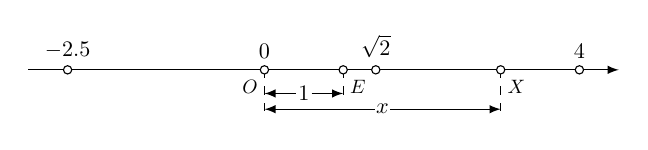
\begin{tikzpicture}
        \draw[-latex] (-3,0) -- (4.5,0);
        \draw[dashed] (0,0) -- (0,-0.6);
        \draw[dashed] (3,0) -- (3,-0.6);
        \draw[dashed] (1,0) -- (1,-0.4);

        \draw[-latex] (0.6,-0.3) -- (1,-0.3);
        \draw[-latex] (0.4,-0.3) -- (0,-0.3);
        \draw[-latex] (1.6,-0.5) -- (3,-0.5);
        \draw[-latex] (1.4,-0.5) -- (0,-0.5);

        \draw[fill=white] (0,0) circle (1.5pt)
        node[above,scale=0.8] at (0,0.05) {$0$}
        node[below left,scale=0.7] at (0,-0.05) {$O$};
        \draw[fill=white] (4,0) circle (1.5pt)
        node[above,scale=0.8] at (4,0.05) {$4$};
        \draw[fill=white] (-2.5,0) circle (1.5pt)
        node[above,scale=0.8] at (-2.5,0.05) {$-2.5$};
        \draw[fill=white] (1,0) circle (1.5pt)
        node[below right,scale=0.7] at (1,-0.05) {$E$};
        \draw[fill=white] (1.414,0) circle (1.5pt)
        node[above,scale=0.8] at (1.414,0.05) {$\sqrt{2}$};
        \draw[fill=white] (3,0) circle (1.5pt)
        node[below right,scale=0.7] at (3,-0.05) {$X$};

        \node[scale=0.8] at (0.5,-0.3) {$1$};
        \node[scale=0.8] at (1.5,-0.5) {$x$};
    \end{tikzpicture}
\end{figure}
则{\kaishu 这条直线上的任意一点 $X$ 必然对应于某一个实数 $x$,} 我们称其为该点的\emph{坐标}\index{zuobiao@坐标}(或横坐标).
若 $X$ 位于自 $O$ 起的正方向上, $x$ 即等于线段 $OX$ 的长度;
而在相反的情形下, 则等于这个长度的负值.

而由几何学上直线的连续性公理,
以点为集合的直线有类似于实数域连续性的性质 [\emph{\ref{subsec:10}}],
因此任意一个实数 $x$ 都必然对应于直线上的某一点.

这样, 在一切实数与有向直线(轴)上的点之间就可以建立起一一对应的关系.
实数可以被表示为轴上的点, 这条轴因此便被称为\emph{数轴}\index{shuzhou@数轴}.

    \chapter{极限论}\label{chap:limits}
\section{数列及其极限}\label{sec:sequence_limits}
\subsection{数列}\label{subsec:22}
在物理学及其他自然科学中我们经常会遇到各种不同的{\kaishu 量}:
时间、长度、体积、重量等.
任一种量, 按照不同的情况, 有时具有不同的值, 有时仅取固定的值.
在第一种情形我们称它为\emph{变量}, 在第二种情形称它为\emph{常量}.

但在数学上我们并不考察量所蕴含的物理意义, 只关心表示这个量的数值.
这样, 对于我们来说, 变量仅为赋予数值的符号(例如字母 $x$)而已.
若变量所能取值的集合 $\X = \{ x\}$ 已经确定, 则这变量就当作是已给定了.
常量可以当作变量的特殊情形来看待, 它相当于 $\X = \{x\}$ 只有一个元素的情形.

在建立变量 $x$ 的极限概念时, 仅知道这变量所取值的数集 $\X$ 还是不够的,
必须再知道它所取的到底是些怎样的数值(在它们中间, 可能有重复的), 以及它取这些值的次序.
一般变量可以按十分复杂的方式变动; 对它的极限作完整讨论, 需要待函数、聚点等概念建立后再进行.
本章先考察最简单而且最重要的一类情形 —— \emph{数列}\index{shulie@数列}
\footnote{原书沿用“整序变量”这一历史术语.
指定整序变量与指定数列在本质上是同一件事:
都是按照某种确定规则, 使每个自然数 $n$ 对应一个确定的实数 $x_n$.
现代数学教材通常使用“数列”, 本书重排本亦统一采用这一名称.}
.

设有自然数的序列
\begin{equation}
    1, 2, \cdots, n, \cdots, n', \cdots \label{eq:natural_seq}
\end{equation}
在该序列中, 数字严格按从小到大的顺序排列着; 若 $n' > n$, 则 $n'$ 位于 $n$ 的后面.
若在序列 \eqref{eq:natural_seq} 内, 按照某种确定的规律, 将每一个自然数 $n$ 对应到一个实数 $x_n$, 我们便得到了数列:
\begin{equation}
    \seq{x}, \cdots, x_{n'}, \cdots \label{eq:real_seq}
\end{equation}
数项 $x_n$ 依序号增大的次序排列着,
也就是说, 当 $n' > n$ 时, $x_{n'}$ 位于 $x_n$ 的后面.
这里所说的是排列的次序, 与 $x_n$ 和 $x_{n'}$ 的大小无关,
$x_{n'}$ 可以大于、小于或等于 $x_n$.

这样得到的对象就是数列, 并将序列 \eqref{eq:real_seq} 简记成 $\{x_n\}$,
它的每一个数值都由一个自然数序号标记, 并且这些数值按序号的先后依次排列.

中学中常见的变量大多属于这一类型.
例如, 等差数列
$$
    \underset{1}{a}, \underset{2}{a+d}, \cdots, \underset{n}{a + (n-1)d}, \cdots
$$
以及等比数列
$$
    \underset{1}{a}, \underset{2}{aq}, \cdots, \underset{n}{aq^{n-1}}, \cdots
$$
都是数列.

再如, 将 $\sqrt{2}$ 的十进制近似值逐位写出:
$$
    \underset{1}{1.4}, \underset{2}{1.41},\underset{3}{1.414},\underset{4}{1.4142}, \cdots
$$
同样得到一个数列.

有时, 数列 $\{x_n\}$ 的第 $n$ 项可以由显式公式直接给出.
在等差数列和等比数列中, 给定序号 $n$, 便可分别由对应的公式算出 $x_n = a + (n-1)d$ 和 $x_n = aq^{n-1}$.
但大多数数列未必有这样简单的通项公式, 然而,
{\kaishu 只要给定初始值和一条确定的递推或计算规则, 能由已有项逐步得到后继项, 该数列仍完全确定.}
例如, 上述 $\sqrt{2}$ 的近似值便可由开方算法逐位求得.
\subsection{数列的极限}\label{subsec:23}
\emph{极限}\index{jixian@极限}的观念贯穿着整个分析课程.
而为了讲极限, 我们总是考察一些变化的量最后的“稳定性”, 这里变量的变化域显然不能是“漫无目的的”,
而应该是由确定的法则规定成\emph{有序的}.
例如, 我们常说的数列
$$
\seq{a}, \cdots
$$
它是按照自然数序列 $1, 2, \cdots, n, \cdots$ 的顺序进行排列.
这种排序自然而然且十分简单, 因此我们先从最简单的数列极限开始讨论.

从直观来看, 一个数列的极限应当是它最后趋于稳定的情况, 例如
$$
\begin{array}{ccccccc}
\phantom{-}1, & \phantom{-}1, & \phantom{-}1, & \phantom{-}1, & \phantom{-}1, & \phantom{-}1, & \cdots \\
\phantom{-}1, & -1, & \phantom{-}1, & -1, & \phantom{-}1, & -1, & \cdots \\
\phantom{-}0, & \phantom{-}1, & \phantom{-}0, & \phantom{-}\dfrac{1}{2}, & \phantom{-}0, & \phantom{-}\dfrac{1}{3}, & \cdots
\end{array}
$$
这三个数列.

第一种情形中, 数列的每一项根本是一个常数, 它的极限应当就是 $1$;
在第二种情形中, 它是由 $1$ 和 $-1$ 两个数交替出现, 最后应当“不稳定”;
第三种情形, 尽管也好像第二种情形那样交替变换,
然而如果先不管 $0$ 这些项,
单独抽离出来的 $\bbbrac{1, \dfrac{1}{2}, \dfrac{1}{3}, \cdots}$ 总会有趋于 $0$ 的趋势,
再加回 $0$ 项, 直觉告诉我们这个数列的极限应当也是 $0$.

然而这种依靠直觉判断的极限显然不严谨, 所以我们应当给出极限严格的定义.

{\kaishu
    若对于任意正数 $\epsilon$, 不论它怎样小, 总存在一个序号 $N$, 使在 $n>N$ 时, 一切 $x_n$ 的值满足不等式
    \begin{equation} \label{eq:sequence_limit_definition}
        \abs{x_n-a}<\epsilon,
    \end{equation}
    则常数 $a$ 称为数列 $\{x_n\}$ 的\emph{极限}.
}

$a$ 是数列极限这一事实, 记成\footnote{lim 是拉丁文 limes 的简写, 指“极限”.}
$$
\limto{n} x_n =a.
$$
我们也说, 数项 $x_n$ \emph{趋于} $a$, 并写成
$$
x_n \to a.
$$
有时也称数列 $\seqset{x}$ \emph{收敛于} $a$.

对于这个定义, 重要的是要认识到, 序号 $N$ 一般来说, 并不是一经指定后就永远不变的,
{\kaishu 它是由我们所选的数 $\epsilon$ 来决定的}.
为了着重强调这一点, 我们有时不写 $N$ 而写成 $N_{\epsilon}$ 来强调 $N$ 与 $\epsilon$ 之间的关系.
需要注意的是, 对给定的 $\epsilon$, 满足条件的 $N$ 并不唯一; 任意更大的序号同样有效.
通常, 随着 $\epsilon$ 减小, 为保证所需精度而选取的阈值也会增大.

数列 $\seqset{x}$ 的一切数值都等于常量 $a$ 的这情形是例外.
显然, 这时 $a = \displaystyle \limto{n} x_n$,
因为这时对于任何 $\epsilon > 0$, 不等式 \eqref{eq:sequence_limit_definition} 能同时对于 $x_n$ 的一切值都成立.

在 \emph{\ref{subsec:17}} 中我们知道, 不等式 \eqref{eq:sequence_limit_definition} 相当于下列不等式
$$
-\epsilon < x_n - a < \epsilon
$$
或
\begin{equation} \label{eq:limit_inequality}
a - \epsilon < x_n < a + \epsilon,
\end{equation}
以后我们经常要用到这些不等式.

若把我们的数列 $\seqset{x}$ 的值及数 $a$, $a \pm \epsilon$ 表示为数轴上的点 [\emph{\ref{subsec:21}}], 则得数列极限一种显明的几何解释.
以 $a$ 点为中心的线段不论取得怎样小(其长为 $2\epsilon$), 一切点 $x_n$, 从某点起, 必全部落在这段之内(这样, 在线段之外一定只有有限个点了).
\begin{figure}[!h]
    \centering
    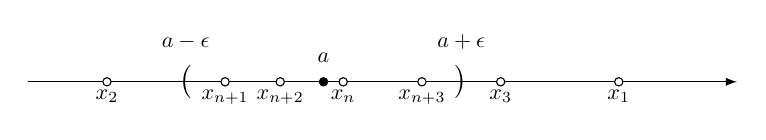
\begin{tikzpicture}
        \draw[-latex] (-4, 0) -- (5, 0);

        \draw[fill=white] (-3, 0) circle (1.5pt) node[below,scale=0.8] {$x_2$};
        \draw[fill=white] (-1.5, 0) circle (1.5pt) node[below,scale=0.8] {$x_{n+1}$};
        \draw[fill=white] (0, 0) circle (1.5pt) node[below,scale=0.8] {$x_n$};
        \draw[fill=white] (2, 0) circle (1.5pt) node[below,scale=0.8] {$x_3$};
        \draw[fill=white] (3.5, 0) circle (1.5pt) node[below,scale=0.8] {$x_1$};
        \draw[fill=white] (-0.8, 0) circle (1.5pt) node[below,scale=0.8] {$x_{n+2}$};
        \draw[fill=white] (1, 0) circle (1.5pt) node[below,scale=0.8] {$x_{n+3}$};

        \draw (-2, 0) node {$ \big( $};
        \draw (-2, 0.5) node[scale=0.8] {$ a-\epsilon $};
        \draw (1.5, 0) node {$ \big) $};
        \draw (1.5, 0.5) node[scale=0.8] {$ a+\epsilon $};

        \draw (-0.25, 0.3) node[scale=0.8] {$ a $};
        \filldraw (-0.25, 0) circle (1.5pt);
    \end{tikzpicture}
\end{figure}

\subsection{无穷小量}\label{subsec:24}
当数列趋向于零时: $x_n\to 0$, 这种情形特别值得注意.

{\kaishu
极限为 $0$ 的数列称为\emph{无穷小量}\index{wuqiongxiao@无穷小量}, 或简称\emph{无穷小}.
}

若在前面数列极限的定义 [\emph{\ref{subsec:23}}] 内使 $a = 0$,
则不等式 \eqref{eq:sequence_limit_definition} 成为
$$
\abs{x_n - 0} = \abs{x_n} < \epsilon \quad (n > N_\epsilon).
$$
这样, 上面无穷小的定义可以不用术语“极限”而更详细地叙述成:
{\kaishu
若数列 $\seqset{x}$ 的绝对值, 自某项起, 成为而且永远保持小于预先指定的任意小的正数 $\epsilon$, 则它称为无穷小.
}

“无穷小”这一历史名称容易引起误解.
除恒等于 $0$ 的平凡情形外, 无穷小数列的某个单独项不能被笼统地称为“很小的量”;
这里描述的是数列的变化过程, 即它的绝对值最终能小于任意预先给定的正数 $\epsilon$.

有了无穷小, 如果设数列 $\seqset{x}$ 以 $a$ 为极限, 则此变量与其极限的差
$$
\alpha_n = x_n - a
$$
显然将为无穷小.

反之, 若 $\alpha_n=x_n-a$ 是无穷小, 则 $x_n \to a$.
因此, $x_n\to a$ 的充分必要条件是差 $\alpha_n=x_n-a$ 为无穷小.
这使我们可以给予“极限”的概念以第二定义:
{\kaishu
若常数 $a$ 与 $x_n$ 的差是无穷小量, 则 $a$ 称为数列 $\seqset{x}$ 的极限.
}

自然而然地, 如果采用极限的第二个定义为极限论的出发点, 则对于无穷小必须应用上述的第二个定义.
否则会产生循环定义: 极限由无穷小确定, 而无穷小又由极限确定.

因此, 若 $x_n \to a$, 则可以表示为
$$
x_n = a + \alpha_n,
$$
式中 $\alpha_n$ 为无穷小.
我们常用这式子以建立数列的极限.

\subsection{例题}\label{subsec:25}
\myrefparagraph{1)}\label{ex:infinitesimal_basic_sequences}
    考察三个数列
    $$
    x_n=\frac{1}{n},\qquad y_n=-\frac{1}{n},\qquad z_n=\frac{(-1)^{n+1}}{n}.
    $$
    它们分别取值为
    $$
    \begin{array}{ccccc}
    \phantom{-}1, & \phantom{-}\dfrac{1}{2}, & \phantom{-}\dfrac{1}{3}, & \phantom{-}\dfrac{1}{4}, & \cdots \\[0.8em]
    -1, & -\dfrac{1}{2}, & -\dfrac{1}{3}, & -\dfrac{1}{4}, & \cdots \\[0.8em]
    \phantom{-}1, & -\dfrac{1}{2}, & \phantom{-}\dfrac{1}{3}, & -\dfrac{1}{4}, & \cdots
    \end{array}
    $$
    要证明这三个数列都是无穷小.

    观察到它们的绝对值都等于 $\dfrac{1}{n}$, 因此当 $n>\dfrac{1}{\epsilon}$ 时, 便有
    $$
    \abs{x_n}<\epsilon,\qquad \abs{y_n}<\epsilon,\qquad \abs{z_n}<\epsilon.
    $$
    这样, 我们取 $\dfrac{1}{\epsilon}$ 的整数部分,
    令 $N_\epsilon = \max\left\{1,\floor{\dfrac{1}{\epsilon}}\right\}$
    \footnote{$\max\{\cdots\}$ 指在所给数中选择最大的那个数,
    但实际情况是 $\epsilon$ 常常是个非常小的数, $\dfrac{1}{\epsilon}$ 将会远远大于 1,
    所以也可以将 $\max$ 省略只保留 $N_\epsilon = \floor{\dfrac{1}{\epsilon}}$; $\floor{p}$ 表示不超过 $p$ 的最大整数, 或简称数 $p$ 的整数部分.},
    就完成了证明.

    注意到第一个变量常大于其极限 0, 第二个常小于 0, 第三个则交迭地忽大于忽小于 0,
    尽管如此, 这都不影响其最终极限为 $0$.

\myrefparagraph{2)}\label{ex:oscillatory_zero_limit}
    若设
    $$
    x_n=\frac{2+(-1)^n}{n}.
    $$
    则数列为
    $$
    1,\ \frac{3}{2},\ \frac{1}{3},\ \frac{3}{4},\ \frac{1}{5},\ \frac{3}{6},\ \ldots.
    $$
    它一会儿靠近 $0$, 一会儿又离开一些, 但仍有
    $$
    \abs{x_n}\leq \frac{3}{n}<\epsilon,
    \qquad
    \text{当 } \ n>\max\left\{1,\floor{\frac{3}{\epsilon}}\right\}\text{ 时}.
    $$
    因而 $x_n\to0$.

\myrefparagraph{3)}\label{ex:zero_odd_terms_limit}
    设
    $$
    x_n=\frac{1+(-1)^n}{n}.
    $$
    这里所有奇数项都等于 $0$, 偶数项为 $2/n$. 由于
    $$
    \abs{x_n}\leq\frac{2}{n}<\epsilon,
    \qquad\text{当 } \ n>\max\left\{1,\floor{\frac{2}{\epsilon}}\right\}\text{ 时},
    $$
    所以 $x_n\to0$.
    数列可以在无穷多个位置恰好取到极限值, 这同样不妨碍极限的存在.

    \ref{ex:infinitesimal_basic_sequences}、 \ref{ex:oscillatory_zero_limit}、 \ref{ex:zero_odd_terms_limit}
    这些简单的例子是很有趣的, 它们体现了数列在趋于极限的方式上的各种可能性.
    无论是变量的值是否均在极限值的一方;
    还是变量是否每一步都向其极限接近;
    又或是变量是否能达到其极限, 即是否具有等于极限的数值;
    这些都不关紧要.
    重要的仅是定义中所说的:
    变量在最后, 即项数充分远时的数值, 与极限值之差要是任意小.
\myrefparagraph{4)}\label{ex:rational_sequence_one_third}
    再来看看更为复杂的例子.
    设
    $$
    x_n=\frac{n^2-n+2}{3n^2+2n-4}.
    $$
    证明 $x_n\to\dfrac{1}{3}$.

    为此直接比较 $x_n$ 与候选极限, 当 $n>2$ 时,
    $$
    x_n-\frac{1}{3}
    =\frac{-5n+10}{3(3n^2+2n-4)}
    $$
    估计其绝对值, 当 $n>2$ 时有
    $$
    \abs{x_n-\frac{1}{3}}
    =\frac{5n-10}{3(3n^2+2n-4)}
    <\frac{5n}{3(3n^2-4)}
    <\frac{5n}{3\cdot2n^2}<\frac{1}{n}.
    $$
    因此取
    $$
    N_\epsilon=\max\left\{2,\floor{\frac{1}{\epsilon}}\right\},
    $$
    这式的结果便小于 $\epsilon$, 这就证明了 $x_n\to\dfrac{1}{3}$.

\myrefparagraph{5)}\label{ex:nth_root_constant_supplement}
    对 $a>1$, 数列
    $$
    x_n=a^{\frac{1}{n}}=\sqrt[n]{a}
    $$
    要证 $x_n\to1$.
    若应用绪论中的 Bernoulli 不等式 \eqref{eq:bernoulli_application}, 则有
    $$
    \abs{x_n-1} = \sqrt[n]{a} - 1 \leq \frac{a-1}{n} < \epsilon,
    \quad \text{当} \ n > N_\epsilon = \max\left\{1,\floor{\dfrac{a-1}{\epsilon}}\right\}.
    $$
    亦可以直接运用对数
    $$
    \abs{x_n-1} = \sqrt[n]{a} - 1 < \epsilon
    \quad\Longleftrightarrow\quad
    \frac{1}{n} < \log_a(1+\epsilon).
    $$
    因此也可以取
    $$
    N_\epsilon=\max\left\{1,\floor{\frac{1}{\log_a(1+\epsilon)}}\right\}.
    $$

    由于所选的方法不同, 我们便得出不同的 $N_\epsilon$ 的表达.
    例如, 在 $ a = 10, \epsilon = 0.01 $ 时, 依第一种方法得
    $
    N_{0.01} = \dfrac{9}{0.01} = 900,
    $
    而依第二种方法得
    $
    N_{0.01} = \floor{\dfrac{1}{0.004 \ 32 \ \cdots}} = 231.
    $
    注意到
    $
    10^{\frac{1}{231}} = 1.010 \, 017 \, \cdots
    $
    与 $1$ 的差已大于 $\varepsilon = 0.01$,
    所以依第二种方法我们得到的 \( N_{0.01}=231 \) 是一切可能的数值中的最小者,
    也就是说为了满足 $ a = 10, \epsilon = 0.01 $ 的条件, 我们的 $N_{0.01}$ 最小只能到 231.
    这在一般情形也是如此, 因为很容易看出, 当
    $
    n \leq \dfrac{1}{\log_a(1 + \varepsilon)}
    $
    时必有
    $
    a^{\frac{1}{n}} - 1 \geq \varepsilon.
    $

    注意: 如果只是要证明极限存在,
    那么我们其实并不需要关心 \( N_\varepsilon \) 最小可能的数值.
    只需保证不等式 \eqref{eq:sequence_limit_definition} 能成立就好了,
    至于从哪一项开始, 位置远些或近些, 可以不必管它.

\myrefparagraph{6)}\label{ex:geometric_infinitesimal}
    若 $\abs{q}<1$, 则数列
    $$
    a_n=q^n
    $$
    是无穷小.

    $q=0$ 时结论显然;
    若 $0<\abs{q}<1$, 证明时只需考虑 $0<\epsilon<1$, 此时
    $$
    \abs{a_n}=\abs{q}^n<\epsilon, \qquad \text{当} \ n>\frac{\ln\epsilon}{\ln\abs{q}} \text{时}.
    $$
    更一般地, 任意常数 $A$ 的数列 $Aq^n$ 也趋于 $0$.

\myrefparagraph{7)}\label{ex:geometric_series_sum}
    再考察无穷等比级数
    $$
    a+aq+aq^2+\cdots+aq^{n-1}+\cdots,\qquad \abs{q}<1.
    $$
    它的前 $n$ 项和为
    $$
    s_n=\frac{a-aq^n}{1-q}=\frac{a}{1-q}-\frac{a}{1-q}q^n.
    $$
    而 $q^n\to0$, 于是它们的和
    $$
    s = \lim_{n\to\infty}s_n=\frac{a}{1-q}.
    $$

\myrefparagraph{8)}\label{ex:averaging_recurrence_limit}
    给定 $x_0=a$、$x_1=b$, 并令
    $$
    x_n=\frac{x_{n-2}+x_{n-1}}{2}\qquad(n\geq2).
    $$
    为了考察这个数列的极限,
    我们将两边同时减去 $x_{n-1}$, 有
    $$
    x_n-x_{n-1}=-\frac{1}{2}(x_{n-1}-x_{n-2}).
    $$
    因而
    $$
    x_n-x_{n-1}=\left(-\frac{1}{2}\right)^{n-1}(b-a),
    $$
    进而
    $$
    x_n=a+(b-a)\sum_{k=0}^{n-1}\left(-\frac{1}{2}\right)^k\qquad(n\geq1).
    $$
    利用等比级数的求和公式, 得到
    $$
    \lim_{n\to\infty}x_n=a+\frac{2}{3}(b-a)=\frac{a+2b}{3}.
    $$

\myrefparagraph{9)}\label{ex:series_partial_sums}
    与等比数列相似, 给定一般数列 $\{a_n\}$, 将它们依次相加, 做成“部分和”
    $$
    A_1 = a_1, \ A_2 = a_1+a_2,\ \cdots,\ A_n=a_1+a_2+\cdots+a_n,\ \cdots
    $$
    若 $A_n\to A$, 就把 $A$ 定义为
    $$
    a_1+a_2+\cdots+a_n+\cdots
    $$
    的和, 上面这个式子也被称为\emph{无穷级数}\index{wuqiongjishu@无穷级数}.
    这时称该级数为\emph{收敛级数}.
    例如
    $$
    \frac{1}{1\cdot2}+\frac{1}{2\cdot3}+\frac{1}{3\cdot4}+\cdots
    $$
    的第 $n$ 个部分和为
    \footnote{$\displaystyle \sum_{k=1}^n a_k$ 是对求和式 $a_1 + a_2 + \cdots + a_n$ 的简写.}
    $$
    A_n=\sum_{k=1}^n\frac{1}{k(k+1)}
    =\sum_{k=1}^n\left(\frac{1}{k}-\frac{1}{k+1}\right)
    =1-\frac{1}{n+1}\to1.
    $$
    因而该级数的和为 $1$.

    \enlargethispage{0.5\baselineskip}
    相反, 如果级数没有有限和, 这时我们就说这个级数\emph{发散}.
    例如
    $$1+1+1+\cdots$$
    就是这样的级数.

\subsection{关于有极限数列的一些定理}\label{subsec:26}
设数列 $\seqset{x}$ 有极限 $a$, 那么由极限定义可知, 对任意 $\epsilon>0$, 从某一项开始都有不等式 \eqref{eq:limit_inequality}:
$$
a - \epsilon < x_n < a + \epsilon,
$$
这一估计可以用来比较数列的后续各项与任意给定常数的大小.
若有数 $p<a$（或 $q>a$）,
都可以选取 $\epsilon<a-p$（或 $\epsilon<q-a$）, 并找到序号 $N$, 使当 $n>N$ 时有
$$
x_n>a-\epsilon > p \qquad \text{（或 }\ x_n<a+\epsilon<q\text{）}.
$$
这样我们就证明了

\myrefparagraph{1\textdegree}\label{prop:eventual_order_from_limit}
{\kaishu 若 $x_n\to a$, 且 $a>p$（或 $a<q$）, 则从某一项开始, 必有
$$
x_n>p \qquad \text{（或 }\ x_n<q\text{）}.
$$}

这一个简单的命题包含一系列有用的推论.

\myrefparagraph{2\textdegree}\label{prop:eventual_sign_preservation}
{\kaishu 若 $x_n\to a$, 且 $a>0$（或 $a<0$）, 则从某一项开始, 必有
$$
x_n>0 \qquad \text{（或 }\ x_n<0\text{）}.
$$}

这被称为收敛数列的\emph{保号性}\index{baohaoxing@保号性}.
它是命题 \ref{prop:eventual_order_from_limit} 在 $p=0$（或 $q=0$）时的直接推论.
更为一般的结果是:
\myrefparagraph{3\textdegree}\label{prop:convergent_sequence_away_from_zero}
{\kaishu 若 $x_n\to a$, 且 $a\neq0$, 则存在正数 $r$ 和自然数 $N$, 使当 $n>N$ 时,
$$
\abs{x_n}>r>0.
$$}

事实上, 当 $a>0 \ (<0)$ 时, 可以取
$$0<p<a \ (a<q<0),$$
再假定 $r=p\ (r=\abs{q})$,
应用命题 \ref{prop:eventual_order_from_limit} 即可.

\myrefparagraph{4\textdegree}\label{prop:convergent_sequence_bounded}
{\kaishu 若数列 $\seqset{x}$ 有有限极限 $a$, 则它必为有界数列, 即存在常数 $M>0$, 使
$$
\abs{x_n}\leq M \qquad (n=1,2,\cdots).
$$}

\enlargethispage{0.5\baselineskip}
取 $M'>\abs{a}$. 由命题 \ref{prop:eventual_order_from_limit}, 存在 $N$, 使当 $n>N$ 时,
$$
-M'<x_n<M',\quad\text{即}\quad \abs{x_n}<M'.
$$
这不等式只可能对于数列的前 $N$ 项(或它们之中的某几项)不满足.
因此只需再令
$$
M=\max\bbbrac{\abs{x_1},\abs{x_2},\ldots,\abs{x_N},M'},
$$
便有 $\abs{x_n}\leq M$ 对一切自然数 $n$ 成立.

\begin{remark}
\myrefparagraph{I.}\label{note:bounded_sequence_equivalent_definition}
数列 $\seqset{x}$ 有界, 也可以等价地写成: 存在两个有限数 $k,g$, 使
$$
k\leq x_n\leq g \qquad (n=1,2,\ldots).
$$
若已知这组不等式, 取 $M=\max\bbbrac{\abs{k},\abs{g}}$, 便有 $\abs{x_n}\leq M$; 反过来, 由 $\abs{x_n}\leq M$ 可得 $-M\leq x_n\leq M$.

\myrefparagraph{II.}\label{note:bounded_not_necessarily_convergent}
命题 \ref{prop:convergent_sequence_bounded} 的逆命题不成立: 有界数列未必收敛. 例如
$$
x_n=(-1)^{n+1}
$$
恒有 $\abs{x_n}=1$, 但它在 $1$ 与 $-1$ 之间交替取值, 没有极限.
\end{remark}

最后可以根据命题 \ref{prop:eventual_order_from_limit} 证明极限的\emph{唯一性}.
\myrefparagraph{5\textdegree}\label{prop:limit_uniqueness}
{\kaishu 数列的极限若存在, 则必定唯一\index{jixiandeweiyixing@极限的唯一性};
也就是说, 一个数列不能同时趋于两个相异的极限. }

用反证法证明. 假设同时有 $x_n\to a$ 和 $x_n\to b$, 并且 $a<b$. 在 $a$ 与 $b$ 之间任取一数 $r$, 使
$$
a<r<b.
$$
由命题 \ref{prop:eventual_order_from_limit}, 存在 $N'$, 使当 $n>N'$ 时有 $x_n<r$; 又存在 $N''$, 使当 $n>N''$ 时有 $x_n>r$. 于是当
$$
n>\max\bbbrac{N',N''}
$$
时, $x_n$ 将同时满足 $x_n<r$ 和 $x_n>r$, 这个矛盾便证明了我们的命题.

\subsection{无穷大量}\label{subsec:27}
\emph{无穷大量}\index{wuqiongdaliang@无穷大量}(或简称\emph{无穷大}),
在某种意义上是与无穷小量相反的量.

{\kaishu
若数列 $\{x_n\}$ 从某项开始, 其绝对值都将大于预先指定的任意大数 $E > 0$,
$$
\abs{x_n} > E \quad (\text{当} \ n > N_E \ \text{时}),
$$
$\seqset{x}$ 便称为无穷大.}

如同无穷小的情形, 所谓“无穷大”, 说的是数列变化的过程, 而不是某一项的数值,
无穷大量中任一个别数值都不能当作“大量”来看待.

最简单的例子是
$$
x_n=n,\quad y_n=-n,\quad z_n=(-1)^{n+1}n.
$$
它们在取定
$
N_E=\floor{E}
$
后, 都能使各自的绝对值大于事先指定的数 $E$.

进一步地可以发现, $\seqset{x}$ 在变化过程中始终带正号,
$\seqset{y}$ 始终带负号, $\seqset{z}$ 则是正负交替出现.
前两种情形可以进一步说明:
{\kaishu 若数列 $\seqset{x}$ 是无穷大量, 并且从某项开始保持一定的符号(+或−),
则按照符号的正或负, 我们说 $\seqset{x}$ 有极限 $+\infty$ 或 $-\infty$, 并写成:
$$
\limto{n}x_n=+\infty,\quad x_n\to+\infty
\qquad\text{或}\qquad
\limto{n}x_n=-\infty,\quad x_n\to-\infty.
$$}
在这两种情形中, 可以分别用不等式
$$
x_n>E \quad\text{或}\quad x_n<-E
$$
来代替 $\abs{x_n}>E$, 作为带确定符号的无穷极限的定义.
一般的无穷大量则统一写成
$$
\abs{x_n}\to+\infty.
$$

因此, 前面例子里的 $\{x_n\}$ 趋向 $+\infty$, $\{y_n\}$ 趋向 $-\infty$.
至于 $\{z_n\}$, 它没有有限极限, 也不趋向 $+\infty$ 或 $-\infty$;
但由于 $\abs{z_n}\to+\infty$, 它仍是一般意义下的无穷大量.

关于这些“广义的数” $\pm\infty$, 我们在 \emph{\ref{subsec:11}} 已讨论过,
它们必须结合上述定义使用, 不能不加条件地当作普通实数进行四则运算.
按照习惯, 语境明确时常用 $\infty$ 代替 $+\infty$.

再看一个无穷大量的例子:
$$
x_n=Q^n,\qquad \abs{Q}>1.
$$
任给 $E>0$, 要使 $\abs{x_n}=\abs{Q}^n>E$, 只需
$$
n\ln\abs{Q}>\ln E, \quad \text{即} \ n>\frac{\ln E}{\ln\abs{Q}}.
$$
因此取
$$
N_E=\max\left\{1,\floor{\frac{\ln E}{\ln\abs{Q}}}\right\}
$$
就证明了我们的命题
\footnote{这里取最大值是为了保证当 $0<E<1$ 时, $N_E$ 仍是正整数.}.
因此, 当 $\abs{Q}>1$ 时, $Q^n$ 是无穷大量.
同样, 当 $Q>1$ 时有 $Q^n\to+\infty$;
当 $Q<-1$ 时, $Q^n$ 的绝对值趋于 $+\infty$, 但它本身没有带符号的无穷极限.

最后, 讲一讲无穷大量与无穷小量间的简单关系:

{\kaishu
若 $\seqset{x}$ 是无穷大量, 则从某项开始必有 $x_n\neq0$.
从这一项起令 $\alpha_n=\dfrac{1}{x_n}$, 并任意补定有限个初始项, 所得数列 $\seqset{\alpha}$ 是无穷小.
}
\begin{proof}
取任意数 $\epsilon>0$. 因 $\abs{x_n}\to+\infty$, 故对于数 $E=\dfrac{1}{\epsilon}$ 可以求得序号 $N$, 使
$$
\abs{x_n}>\frac{1}{\epsilon}\qquad(n>N).
$$
于是对于这样的 $n$, 有
$$
\abs{\alpha_n} = \abs{\frac{1}{x_n}} < \epsilon,
$$
这就证明了我们的命题.
\end{proof}

仿此, 可以证明逆命题:

{\kaishu
若无穷小数列 $\seqset{\alpha}$ 的各项均不为 $0$, 则其倒数 $x_n=\dfrac{1}{\alpha_n}$ 是无穷大量.
}

\begin{remark}
引入无穷极限并不会破坏命题 \ref{prop:limit_uniqueness} 中建立的极限的唯一性.
由命题 \ref{prop:convergent_sequence_bounded}, 有有限极限的数列必定有界;
与之相反的, 我们可以建立无界的概念:

若不存在常数 $M>0$, 使 $\abs{x_n}\leq M$ 对一切自然数 $n$ 成立,
就称数列 $\seqset{x}$ \emph{无界}\index{wujieshulie@无界数列}.
这等价于:
{\kaishu 任给 $E>0$ 和自然数 $N$, 总能找到某个 $n>N$, 使
$$
\abs{x_n}>E.
$$}
很明显看出, 无穷大量一定是无界的.
因此, 一个数列不可能既有有限极限, 又趋于无穷.

但是无界数列与无穷大却不是等价的,
最关键的点在于无界数列中的序号 $n$ 可以随 $E$ 和 $N$ 改变,
并不要求从某项开始, 所有项的绝对值都大于 $E$.
例如, 数列
$$
x_n=\begin{cases}
    n, & n\text{ 为偶数},\\
    0, & n\text{ 为奇数}
\end{cases}
$$
是无界的, 因为它的偶数项可以任意大;
但它含有无穷多个等于 $0$ 的项, 因而并不趋于无穷.

这说明“无界”比“无穷大”弱.
换言之, {\kaishu 无穷大量一定无界, 但无界数列未必是无穷大量. }
\end{remark}

\begin{comment}
\section{极限的定理·若干容易求得的极限}
\subsection{比较性} {\kaishu 若两个数列 $\seqset{x} , \seqset{y}$ 对应项常满足不等式 $x_n \geq y_n$, 并且各趋于有限极限:
$$
\limto{n} x_n = a, \quad \limto{n} y_n = b,
$$
则必 $a \geq b$.}

假定是相反的情形: 设 $a < b$.
任取在 $a$ 与 $b$ 间的一数 $r$, $a < r < b$.
那么, 一方面, 可以求得序号 $N'$, 使当 $n > N'$ 时成立 $x_n < r$;
另一方面, 又可求得序号 $N''$, 使当 $n > N''$ 时成立 $y_n > r$.
若 $N$ 大于 $N'$ 和 $N''$, 则当 $n > N$ 时将同时成立不等式
$$
x_n < r, \quad y_n > r \Rightarrow x_n < y_n,
$$
这与假定矛盾.

比较性使得我们得以对不等式(连同着等号的)取极限: 由 $x_n \geq y_n$ 得结论:
$$
\limto{n} x_n \geq \limto{n} y_n.
$$
当然, 各处的 $\geq$ 号都可以换成 $\leq$ 号.

请注意, 由严格的不等式 $x_n > y_n$, 一般说来, 不能推得严格的不等式 $\displaystyle \limto{n} x_n > \limto{n} y_n$, 而仅能推得: $\displaystyle \limto{n} x_n \geqslant \limto{n} y_n$.

例如, 对于一切的自然数 $n$, 都有 $\displaystyle \frac{1}{n} > -\frac{1}{n}$, 但
$$
\limto{n} \frac{1}{n} = \limto{n} \brac{-\frac{1}{n}} = 0.
$$
最后的极限并不是严格大于.

\subsection{夹逼准则}
{\kaishu 若 $x_n, y_n, z_n$ 恒满足不等式
$$
x_n \leqslant y_n \leqslant z_n,
$$
并且 $x_n$ 及 $z_n$ 趋向同一极限 $a$:
$$
\limto{n} x_n = \limto{n} z_n = a,
$$
则 $y_n$ 亦必以 $a$ 为极限:
$$
\limto{n} y_n = a.
$$}

指定任意的 $\epsilon > 0$. 对于这 $\epsilon$, 首先可以求得序号 $N'$, 使当 $n > N'$ 时
$$
a - \epsilon < x_n < a + \epsilon.
$$
其次, 又可求得序号 $N''$, 使当 $n > N''$ 时
$$
a - \epsilon < z_n < a + \epsilon.
$$
设 $N$ 大于 $N'$ 及 $N''$, 则当 $n > N$ 时, 上述两不等式都能满足, 故
$$
a - \epsilon < x_n \leqslant y_n \leqslant z_n < a + \epsilon.
$$
结果当 $n > N$ 时
$$
a - \epsilon < y_n < a + \epsilon \quad \text{或} \quad \abs{y_n - a} < \epsilon.
$$
这样, 实际上就是 $\displaystyle \limto{n} y_n = a$.

\subsection{无穷小引理}
在后面极限的中我们将要同时考虑两个(或更多个)数列极限, 并在它们之间施行算术运算.
在证明关于极限的算术运算的性质时, 下面两个关于无穷小的引理, 将担任着重要的角色.

\begin{lemma} \label{n0}
    任何有限个无穷小的和亦是无穷小量.
\end{lemma}

\begin{proof}
我们只证明对于二无穷小 $\alpha_n$ 及 $\beta_n$ 的情形(一般的情形仿此讨论).

给定任意的 $\epsilon > 0$.
根据无穷小的定义, 由 $\epsilon$ 可以决定无穷小 $\alpha_n$ 的序号 $N'$, 以及关于 $\beta_n$ 的序号 $N''$, 使当 $n > N', N''$ 时有
$$
\abs{\alpha_n} < \frac{\epsilon}{2}, \quad \abs{\beta_n} < \frac{\epsilon}{2}.
$$
若取自然数 $N$ 大于 $N'$ 及 $N''$, 则当 $n > N$ 时, 两不等式同时成立, 这样, 便有
$$
\abs{\alpha_n + \beta_n} \leqslant \abs{\alpha_n} + \abs{\beta_n} < \frac{\epsilon}{2} + \frac{\epsilon}{2} = \epsilon.
$$
因此, $\alpha_n + \beta_n$ 也是无穷小.
\end{proof}

\begin{lemma} \label{a0}
    有界变量 $x_n$ 与无穷小 $\alpha_n$ 的乘积仍是无穷小.
\end{lemma}

\begin{proof}
设对于一切 $n$ 有
$$
\abs{x_n} \leqslant M \quad (M > 0).
$$
若给定任意数 $\epsilon > 0$, 则依 $\dfrac{\epsilon}{M}$, 对于无穷小 $\alpha_n$ 可以求出 $N$, 使当 $n > N$ 时有
$$
\abs{\alpha_n} < \frac{\epsilon}{M}.
$$
对于这种 $n$, 显然有
$$
\abs{x_n \cdot \alpha_n} = \abs{x_n} \cdot \abs{\alpha_n} < M \cdot \frac{\epsilon}{M} = \epsilon.
$$
由此推得, $x_n \cdot \alpha_n$ 为无穷小.
\end{proof}

\subsection{四则运算}
有了上述两个引理, 我们便可以叙述极限的四则运算, 有了它们便可以不必把一切与极限有关的问题都追溯到“极限”的定义, 然后依指定的 $\epsilon$ 找出对应的 $N$ 等等, 使得极限的计算将大为简化.

1\textdegree~
{\kaishu 若数列 $\{x_n\}$ 及 $\{y_n\}$ 趋于有限极限:
$$
\limto{n} x_n = a, \quad \limto{n} y_n = b,
$$
则它们的和(差)仍趋于有限极限, 并且
$$
\limto{n} \brac{x_n \pm y_n} = a \pm b.
$$}

由极限的第二定义, 推得
$$
x_n = a + \alpha_n, \quad y_n = b + \beta_n
$$
式中 $\alpha_n$ 及 $\beta_n$ 为无穷小. 故
$$
x_n \pm y_n = (a \pm b) + (\alpha_n \pm \beta_n).
$$
这里的 $\alpha_n \pm \beta_n$ 依引理 \ref{n0} 为无穷小.
因此, 应用极限的第二定义, 可以证明 $x_n \pm y_n$ 有极限 $a \pm b$.

这定理及其证法, 可以推广到任意有限个有极限的数列相加的情形.

2\textdegree~
{\kaishu 若数列 $\{x_n\}$ 及 $\{y_n\}$ 趋于有限极限:
$$
\limto{n} x_n = a, \quad \limto{n} y_n = b,
$$
则它们的积仍趋于有限极限, 并且
$$
\limto{n} x_n y_n = ab.
$$}

仍由极限的第二定义, 这次便有
$$
x_n y_n = ab + (a\beta_n + b\alpha_n + \alpha_n\beta_n).
$$
依引理 \ref{n0} 及 \ref{a0}, 在括号内的式子为无穷小量.由此便推得, $x_n y_n$ 确趋于极限 $ab$.

这定理同样可以推广到任意有限个有极限的数列相乘的情形.

3\textdegree~
{\kaishu 若数列 $\{x_n\}$ 及 $\{y_n\}$ 趋于有限极限:
$$
\limto{n} x_n = a, \quad \limto{n} y_n = b,
$$
并且 $b$ \emph{异于} 0, 则它们的比仍趋于有限极限, 并且
$$
\limto{n} \frac{x_n}{y_n} = \frac{a}{b}.
$$}

由于 $b \neq 0$, 根据保号性, 由某项开始, 不仅 $y_n \neq 0$, 且有
$$
\abs{y_n} > r > 0,
$$
式中 $r$ 是常数.
对于使上面的不等式成立的那些 $n$, 比 $\dfrac{x_n}{y_n}$ 显然是有意义的.

依旧从极限的第二定义出发, 得
$$
\frac{x_n}{y_n} - \frac{a}{b} = \frac{a + \alpha_n}{b + \beta_n} - \frac{a}{b} = \frac{1}{by_n}(b\alpha_n - a\beta_n).
$$

依引理 \ref{n0} 及 \ref{a0}, 在括号内的式子 $b\alpha_n - a\beta_n$ 为无穷小量.
根据开始时的叙述, 而其乘数将是有界变量:
$$
\abs{\frac{1}{by_n}} = \frac{1}{\abs{b}\abs{y_n}} < \frac{1}{\abs{b}r}.
$$
因此, 依引理 \ref{a0}, 等式右边的积将是无穷小.
但它表示 $\dfrac{x_n}{y_n}$ 及数 $\dfrac{a}{b}$ 的差, 故 $\dfrac{x_n}{y_n}$ 的极限是 $\dfrac{a}{b}$.
此即所要证的.

\subsection{未定式}
上面我们讨论了
$$
x_n \pm y_n, \quad x_ny_n, \quad \frac{x_n}{y_n},
$$
并在 $\seqset{x}$ 及 $\seqset{y}$ 都趋于有限极限的假定下在相除的情形, $\seqset{y}$ 的极限应不等于零, 各式子的极限.

今再详述余下的尚未考虑的情形, 当 $\seqset{x}$ 及 $\seqset{y}$ (其中之一或两者) 的极限是无穷大时, 或(若论及除法)当分母的极限为零时.
由这两种情形, 这里讲述四种重要而且有用的未定式.

1\textdegree~
我们首先来看商 $\dfrac{x_n}{y_n}$, 设 $\seqset{x}$ 及 $\seqset{y}$ 同时趋于零.
下面给出三种情况:

设 $x_n = \dfrac{1}{n^2}, y_n = \dfrac{1}{n}$, 则两数列各自趋于零, 它们的比 $\dfrac{x_n}{y_n} = \dfrac{1}{n}$ 也趋于零; 反之, 设 $x_n = \dfrac{1}{n}, y_n = \dfrac{1}{n^2}$, 虽然它们依旧各自趋于零, 但这次它们的比 $\dfrac{x_n}{y_n} = n$ 趋于 $\infty$.

再取任一异于零的数 $a$, 并作出两个无穷小 $x_n = \dfrac{a}{n}$ 及 $y_n = \dfrac{1}{n}$ 便知它们的比有极限为 $a$.

最后, 若 $x_n = \dfrac{(-1)^{n+1}}{n}, y_n = \dfrac{1}{n}$ (两者各有极限为零), 则比 $\dfrac{x_n}{y_n} = (-1)^{n+1}$ 没有极限.

这样, 单知道 $\seqset{x}$ 及 $\seqset{y}$ 的极限 0, 在目前的情形下我们无法判断它们的比的极限, 必须知道数列本身改变的规律, 并直接研究比 $\dfrac{x_n}{y_n}$.
为了要表达当 $x_n \to 0$ 及 $y_n \to 0$ 的情形时的未定性, 就说, {\kaishu 表达式 $\dfrac{x_n}{y_n}$ 是 $\dfrac{0}{0}$ 型的未定式}.

2\textdegree~
在同时 $x_n \to \pm \infty$ 及 $y_n \to \pm \infty$ 的情形, 亦有类似的情况.
若不知数列本身, 关于它们的比的极限便不能作出一般的论断.
这一事实可以用完全类似于 1\textdegree 内引用的那些例题来表明:
\begin{align*}
    &x_n = n \to \infty, \quad y_n = n^2 \to \infty, \quad \frac{x_n}{y_n} = \frac{1}{n} \to 0; \\
    &x_n = n^2 \to \infty, \quad y_n = n \to \infty, \quad \frac{x_n}{y_n} = n \to \infty; \\
    &x_n = an \to \pm \infty \quad (a \neq 0), \quad y_n = n \to \infty, \quad \frac{x_n}{y_n} = a \to a; \\
    &x_n = [2 + (-1)^{n+1}]n \to \infty, \quad y_n = n \to \infty, \quad \frac{x_n}{y_n} = 2 + (-1)^{n+1} \ \text{发散}
\end{align*}

在这种情况下, 就说, {\kaishu 表达式 $\dfrac{x_n}{y_n}$ 是 $\dfrac{\infty}{\infty}$ 型的未定式}.

3\textdegree~
若 $\seqset{x}$ 趋于零, 同时 $\seqset{y}$ 趋于 $\pm \infty$, 则研究积 $x_n y_n$ 的极限时, 我们又遇到像 1\textdegree 及 2\textdegree 内所遇到的那种未定性. 关于这点可以由下面的例题证实它:
\begin{align*}
    &x_n = \frac{1}{n^2} \to 0, \quad y_n = n \to \infty, \quad x_n y_n = \frac{1}{n} \to 0; \\
    &x_n = \frac{1}{n} \to 0, \quad y_n = n^2 \to \infty, \quad x_n y_n = n \to \infty; \\
    &x_n = \frac{a}{n} \to 0 \quad (a \neq 0), \quad y_n = n \to \infty, \quad x_n y_n = a \to a; \\
    &x_n = \frac{(-1)^{n+1}}{n} \to 0, \quad y_n = n \to \infty, \quad x_n y_n = (-1)^{n+1} \ \text{发散}
\end{align*}

在这种情况下, 就说, {\kaishu 表达式 $x_n y_n$ 是 $0 \cdot \infty$ 型的未定式}.

4\textdegree~
这里讲当 $\seqset{x}$ 及 $\seqset{y}$ 趋于异号的无穷大时, 若不知道 $x_n$ 及 $y_n$ 本身, 也不可能确定 $x_n + y_n$ 的极限. 在这里所表示的各种不同的可能性可用下面的例题表明它:
\begin{align*}
    &x_n = 2n \to +\infty, \quad y_n = -n \to -\infty, \quad x_n + y_n = n \to +\infty; \\
    &x_n = n \to +\infty, \quad y_n = -2n \to -\infty, \quad x_n + y_n = -n \to -\infty; \\
    &x_n = n + a \to +\infty, \quad y_n = -n \to -\infty, \quad x_n + y_n = a \to a; \\
    &x_n = n + (-1)^{n+1} \to +\infty, \quad y_n = -n \to -\infty, \quad x_n + y_n = (-1)^{n+1} \ \text{发散}
\end{align*}

因此, 当 $x_n \to +\infty$ 及 $y_n \to -\infty$ 时, 即说, {\kaishu 表达式 $x_n + y_n$ 是 $\infty - \infty$ 型的未定式}.

综合上面所讨论, 当提出了依 $\seqset{x}$ 及 $\seqset{y}$ 的极限去确定由它们所组成的四则运算的极限这个问题以后, 我们可以发现不可能解答的四种情形: 即型为
$$
\frac{0}{0}, \quad \frac{\infty}{\infty}, \quad 0 \cdot \infty, \quad \infty - \infty
$$
的\emph{未定式}.在这些情形, 必须注意数列 $\seqset{x}$ 及 $\seqset{y}$ 的改变规律, 直接去研究我们所关心的式子.
类似的研究称为\emph{未定式的定值法}.
以后它并不永远像上面所举的例题那样简单.

将已给式子\emph{变形}以消除其“未定性”是未定式定值法中常用的方法.

\begin{example}
    考察这么一个极限, 设 $p(n)$ 是整数 $n$ 的常系数多项式:
    $$
    p(n) = a_0n^k + a_1n^{k-1} + \cdots + a_{k-1}n + a_k,
    $$
    若这多项式的一切系数全是正(负)的, 则显然 $p(n)$ 的极限是 $+\infty$ ($-\infty$).
    但在系数为异号的情形, 某些项趋向 $+\infty$, 另一些项趋向 $-\infty$, 就遇到 $\infty - \infty$ 型的未定式.

    要确定这一未定式, 可以把 $p(n)$ 写成
    $$
    p(n) = n^k \brac{a_0 + \frac{a_1}{n} + \cdots + \frac{a_{k-1}}{n^{k-1}} + \frac{a_k}{n^k}}.
    $$
    因为在括号内的一切加数, 从第二项起, 当 $n$ 增大时为无穷小, 所以括号内的式子有极限为 $a_0$.
    第一个乘数趋向 $+\infty$. 则整个式子趋于 $+\infty$ 或 $-\infty$, 结果视 $a_0$ 的符号而定.
\end{example}

\begin{example}
    若 $q(n)$ 也是多项式:
    $$q(n) = b_0n^l + b_1n^{l-1} + \cdots + b_{l-1}n + b_l, $$
    则商 $\dfrac{p(n)}{q(n)}$ 在 $n\to\infty$ 时是 $\dfrac{\infty}{\infty}$ 型的未定式.

    在这里也就将每一个多项式变形, 如同在上例内做过的那样, 则得:
    $$
    \frac{p(n)}{q(n)} = n^{k-l} \frac{a_0 + \dfrac{a_1}{n} + \cdots + \dfrac{a_k}{n^k}}{b_0 + \dfrac{b_1}{n} + \cdots + \dfrac{b_l}{n^l}}.
    $$
    上式右边第二个乘数有一有限极限 $\dfrac{a_0}{b_0}$.
    若两个多项式的幂次相等: $k = l$, 则比 $\dfrac{p(n)}{q(n)}$ 的极限为 $\dfrac{a_0}{b_0}$.
    当 $k > l$ 时, 第一个乘数趋向 $\infty$, 故所考察的比亦趋向 $\pm\infty$ (其符号视 $\dfrac{a_0}{b_0}$ 的符号而定).
    最后, 当 $k < l$ 时, 第一个乘数趋向零, 于是整个式子跟着它趋向零.
\end{example}

\begin{example}
    证明, 在 $0 < k < 1$ 时,
    $$
    \limto{n} [(n+1)^k - n^k] = 0.
    $$

    这里是 $\infty - \infty$ 型的未定式.
    进行变形:
    $$
    0 < (n+1)^k - n^k = n^k \bbrac{\brac{1 + \frac{1}{n}}^k - 1} < n^k \bbrac{\brac{1 + \frac{1}{n}} - 1} = \frac{1}{n^{1-k}}.
    $$
    因 $\dfrac{1}{n^{1-k}} \to 0$, 所以 $(n+1)^k - n^k \to 0$, 此即所要证的.
\end{example}

\begin{example}
    求
    $$
    x_n = \sqrt{n}(\sqrt{n+1}-\sqrt{n})
    $$
    的极限.
    根据上例, $x_n$ 是 $0\cdot\infty$ 的未定式.

    经过变形:
    $$
    x_n = \sqrt{n} \cdot \frac{(\sqrt{n+1}-\sqrt{n})(\sqrt{n+1}+\sqrt{n})}{\sqrt{n+1}+\sqrt{n}} = \frac{\sqrt{n}}{\sqrt{n+1}+\sqrt{n}} = \frac{1}{\sqrt{1+1/n}+1} \to \frac{1}{2}.
    $$
\end{example}

\begin{example}
    求出下列数列的极限:
    $$
    x_n = \frac{n}{\sqrt{n^2 + n}}, \quad y_n = \frac{n}{\sqrt{n^2 + 1}},
    $$
    及
    $$
    z_n = \frac{1}{\sqrt{n^2 + 1}} + \frac{1}{\sqrt{n^2 + 2}} + \cdots + \frac{1}{\sqrt{n^2 + i}} + \cdots + \frac{1}{\sqrt{n^2 + n}}.
    $$

    容易看出, $x_n$ 及 $y_n$ 是 $\dfrac{\infty}{\infty}$ 型的未定式(因两者中的根式都 $> n$, 故它们必趋向 $\infty$).
    将它们变形, 用 $n$ 除分子及分母:
    $$
    x_n = \frac{1}{\sqrt{1 + 1/n}} \to 1, \quad y_n = \frac{1}{\sqrt{1 + 1/n^2}} \to 1.
    $$

    $z_n$ 的表示式有着特有的形式: 这个和的每一项都依赖于 $n$, 且其项数也随着 $n$ 而增大.
    因每一项都小于首项而大于末项, 故
    $$
    \frac{n}{\sqrt{n^2 + n}} < z_n < \frac{n}{\sqrt{n^2 + 1}},
    $$
    即 $x_n < z_n < y_n$.
    因此, 依夹逼准则, $z_n$ 亦必趋于极限 1.
\end{example}

\begin{example}
    设给定 $m$ 个正数 $a_1, a_2, \cdots, a_m$, 其中之最大者记成 $A$, 证明
    $$
    \limto{n} \sqrt[n]{a_1^n + a_2^n + \cdots + a_m^n} = A.
    $$

    这一结论可由很明显的不等式
    $$
    A \leq \sqrt[n]{a_1^n + a_2^n + \cdots + a_m^n} \leq A \cdot \sqrt[n]{m}
    $$
    推得.
\end{example}

\begin{example} \label{muchbigger}
    今研究比
    $$
    \frac{a^n}{n^k}, \quad \frac{\log_a n}{n^k}
    $$
    的极限(当 $k \geq 1$ 时), 它们都是 $\dfrac{\infty}{\infty}$ 型的未定式.

    对于第一个极限, 先证一辅助不等式.
    令 $a = 1 + \lambda$, 因此 $\lambda > 0$, 依Newton二项公式得:
    $$
    a^n = (1 + \lambda)^n = 1 + n\lambda + \frac{n(n-1)}{2}\lambda^2 + \cdots > \frac{n(n-1)}{2}\lambda^2.
    $$
    因在 $n > 2$ 时, 显然 $n - 1 > \dfrac{n}{2}$, 故最后得出
    $$
    \frac{a^n}{n} > \frac{(a-1)^2}{4} n.
    $$

    在 $k = 1$ 时, 立即得出
    $$
    \frac{a^n}{n} > \frac{(a-1)^2}{4} n \to \infty.
    $$
    这一结果对于任何 $a > 1$ 均成立, 故若 $k > 1$, 便可写成(至少在充分大的 $n$ 时)
    $$
    \frac{a^n}{n^k} = \bbrac{\frac{(a^{\frac{1}{k}})^n}{n}}^k > \frac{(a^{\frac{1}{k}})^n}{n} \to \infty,
    $$
    由此
    $$
    \limto{n} \frac{a^n}{n^k} = +\infty \quad (a > 1).
    $$

    对于第二个极限, 我们仅需考虑 $k=1$ 的情况.
    实际上, 若取任意数 $\epsilon > 0$, 则根据 $a^\epsilon > 1$, 当 $n$ 充分大时将有
    $$
    \sqrt[n]{n} < a^\epsilon.
    $$
    以 $a$ 为底取对数, 便得
    $$
    \frac{\log_a n}{n} < \epsilon.
    $$
    由此便推得上述命题.

    这两个极限告诉我们, 指数, 幂和对数在无穷处的极限性态, 我们记做
    $$
    \text{指数} \gg \text{幂} \gg \text{对数}.
    $$
\end{example}

\subsection{Stolz 定理} 为着要确定 $\dfrac{\infty}{\infty}$ 或 $\dfrac{0}{0}$ 型未定式的极限, 下面这个定理是经常有用的:
\begin{theorem}($\dfrac{*}{\infty}$)
    设 $y_n \to +\infty$, 并且从某一项开始, 在 $n$ 增大时 $y_n$ 亦增大: $y_{n+1} > y_n$. 则
    $$
    \limto{n} \frac{x_n}{y_n} = \limto{n} \frac{x_n - x_{n-1}}{y_n - y_{n-1}}
    $$
    只需等式右边的极限已知为存在(有限或 $\pm \infty$).
\end{theorem}
\begin{proof}
    首先假定这极限等于有限数 $l$:
    $$
    \limto{n} \frac{x_n - x_{n-1}}{y_n - y_{n-1}} = l
    $$

    则依任何已给的 $\epsilon > 0$, 必能求得序号 $N$, 使当 $n > N$ 时有
    $$
    \abs{\frac{x_n - x_{n-1}}{y_n - y_{n-1}} - l} < \frac{\epsilon}{2}
    $$
    或
    $$
    l - \frac{\epsilon}{2} < \frac{x_n - x_{n-1}}{y_n - y_{n-1}} < l + \frac{\epsilon}{2}
    $$
    意即, 不论取怎样的 $n > N$, 一切分数
    $$
    \frac{x_{N+1} - x_N}{y_{N+1} - y_N}, \frac{x_{N+2} - x_{N+1}}{y_{N+2} - y_{N+1}},  \cdots,  \frac{x_{n-1} - x_{n-2}}{y_{n-1} - y_{n-2}},  \frac{x_n - x_{n-1}}{y_n - y_{n-1}}
    $$
    都包含在这些限界之内. 因为 $n$ 增大时 $y_n$ 随着增大, 它们的分母都是正数, 所以在那些限界之内亦包含着分数
    $$
    \frac{x_n - x_N}{y_n - y_N}
    $$
    它的分子即为上述各分式的一切分子的和, 分母即为一切分母的和. 因此, 在 $n > N$ 时,
    $$
    \abs{\frac{x_n - x_N}{y_n - y_N} - l} < \frac{\epsilon}{2}
    $$

    由恒等式:
    $$
    \frac{x_n}{y_n} - l = \frac{x_N - ly_N}{y_n} + \brac{1 - \frac{y_N}{y_n}} \brac{\frac{x_n - x_N}{y_n - y_N} - l}
    $$
    可得
    $$
    \abs{\frac{x_n}{y_n} - l} \leqslant \abs{\frac{x_N - ly_N}{y_n}} + \abs{\frac{x_n - x_N}{y_n - y_N} - l}
    $$

    右边的第二项, 我们已看到, 在 $n > N$ 时 $< \dfrac{\epsilon}{2}$; 由于 $y_n \to +\infty$, 所以第一项, 在 $n > N'$ 时, 也将 $< \dfrac{\epsilon}{2}$. 若在这时所取的 $N' > N$, 则在 $n > N'$ 时, 显然有
    $$
    \abs{\frac{x_n}{y_n} - l} < \epsilon,
    $$
    这就证明了我们的命题.

    而无穷极限的情形可以化为上面已研究过的情形. 例如, 设
    $$
    \limto{n} \frac{x_n - x_{n-1}}{y_n - y_{n-1}} = +\infty.
    $$
    由此, 首先推得(在充分大的 $n$ 时),
    $$
    x_n - x_{n-1} > y_n - y_{n-1},
    $$
    因此, 随着 $y_n \to +\infty$ 而 $x_n \to +\infty$, 并且 $x_n$ 随着序号 $n$ 的增大而无限制增大. 在这种情况下, 可以把已证明的定理应用于
    $$
    \limto{n} \frac{y_n}{x_n} = \limto{n} \frac{y_n - y_{n-1}}{x_n - x_{n-1}} = 0.
    $$
    因为在这里极限已是有限的, 由此推得
    $$
    \limto{n} \frac{x_n}{y_n} = +\infty,
    $$
    此即所要证的.
\end{proof}

我们知道, 无穷大量的倒数是无穷小量, 则对于 Stolz 定理的分子分母同时进行倒数处理(在倒数后, 增大的性质应当变为减小的性质), 可以得到
\begin{theorem}($\dfrac{*}{0}$)
    设 $\seqset{y}$ 是无穷小, 且从某一项开始, 在 $n$ 增大时 $y_n$ 减小: $y_{n+1} < y_n$.则
    $$
    \limto{n} \frac{x_n}{y_n} = \limto{n} \frac{x_n - x_{n-1}}{y_n - y_{n-1}}
    $$
    只需等式右边的极限已知为存在(有限或 $\pm \infty$).
\end{theorem}

应用 Stolz 定理可以得到下面这个 Cauchy 命题
\begin{proposition} \label{Cauchy_Proposition}
    若数列 $\{a_n\}$ 有(有限或无穷)极限, 则
    $$
    b_n = \frac{a_1 + a_2 + \cdots + a_n}{n}
    $$
    (数列 $\{a_n\}$ 的首 $n$ 个值的“算术平均值”)亦有同一极限.
\end{proposition}

实际上, 在 Stolz 定理内令
$$
x_n = a_1 + a_2 + \cdots + a_n, \quad y_n = n,
$$
便有
$$
    \limto{n} b_n = \limto{n} \frac{x_n}{y_n} = \limto{n} \frac{x_n - x_{n-1}}{y_n - y_{n-1}} = \limto{n} a_n.
$$
例如,
$$
    \limto{n} \frac{1+\sqrt{2}+\sqrt[3]{3}+\cdot + \sqrt[n]{n}}{n} = \limto{n} \sqrt[n]{n} = 1.
$$

\begin{example}
    计算
    $$
    \limto{n} z_n = \limto{n} \frac{1^k + 2^k + ... + n^k}{n^{k+1}} , \quad k \text{为自然数.}
    $$
\end{example}
令
$$
x_n = 1^k + 2^k + \cdots + n^k, \quad y_n = n^{k+1},
$$
便有
$$
    \limto{n} z_n = \limto{n} \frac{n^k}{n^{k+1} - (n-1)^{k+1}}.
$$
由二项式展开:
$$
(n-1)^{k+1} = n^{k+1} - (k+1)n^k +  \cdots
$$
如此, 便有
$$
n^{k+1} - (n-1)^{k+1} = (k+1)n^k - \cdots
$$
从而
$$
    \limto{n} z_n = \limto{n} \frac{n^k}{(k+1)n^k + \cdots } = \frac{1}{k+1}.
$$

\begin{example}
    计算
    $$
    u_n = n \brac{z_n - \frac{1}{k+1}} = \frac{1^k + 2^k + \cdots + n^k}{n^k} - \frac{n}{k+1}
    $$
    的极限.
\end{example}
简单化简得:
$$
u_n = \frac{(k+1)(1^k + 2^k + \cdots + n^k) - n^{k+1}}{(k+1)n^k}.
$$
令 $x_n$ 等于分子, $y_n$ 等于分母, 应用 Stolz 定理:
$$
    \limto{n} u_n = \limto{n} \frac{(k+1)n^k - [n^{k+1} - (n-1)^{k+1}]}{(k+1)[n^k - (n-1)^k]}.
$$
对分子进行二项式展开:
\begin{align*}
(k+1)n^k  - [n^{k+1} - (n-1)^{k+1}]
&= (k+1)n^k - \bbrac{(k+1)n^k - \binom{k+1}{2}n^{k-1} + \cdots} \\
&= \binom{k+1}{2}n^{k-1} + \cdots = \frac{(k+1)k}{2}n^{k-1} + \cdots
\end{align*}
对分母进行二项式展开:
$$
n^k - (n-1)^k = kn^{k-1} - \cdots
$$
最后即得
$$
    \limto{n} u_n = \limto{n} \frac{\dfrac{(k+1)k}{2}n^{k-1} + \cdots}{(k+1)kn^{k-1} + \cdots } = \frac{1}{2}.
$$

\section{单调数列}
\subsection{单调数列的极限}
到目前为止, 我们所学的极限存在的定理中, 都是先假设存在, 再去根据某些表达式去计算这个极限.
如果能用定义直接说明自然是十分完美, 但是定义的过程非常繁琐, 我们一般都不用其去说明.
有些情况下, 我们假设了极限的存在性, 并且也确实求出了某个极限, 但是这个极限真的存在吗?
这句话看起来有点绕口, 我们以一个例子进行说明:

由某一实数 $c$ 出发, 假定 $x_1 = \dfrac{c}{2}$, 数列 $\{x_n\}$ 有递推式
\begin{equation} \label{monotone_ex1}
    x_{n+1} = \frac{c}{2} + \frac{x_n^2}{2}.
\end{equation}

我们假设 $\seqset{x}$ 有极限存在, 是为 $a$, 那么上式两边同时取极限, 应当有
$$
a = \frac{c}{2} + \frac{a^2}{2}.
$$
由这二次方程求得
\begin{equation} \label{monotone_ex2}
    a_{\pm} = 1 \pm \sqrt{1 - c}.
\end{equation}
由此立刻看出, 在 $c > 1$ 时这个实数列极限是个带有 $\i$ 的复数, 这是不可能的, 从而极限不存在.
这里用了“反证法”, 所以可以直接下结论说 $c > 1$ 原数列必定没有极限.

但是到 $c \leq 1$ 的情况就不行了, 我们已假设了极限存在并且也求出了所谓极限 $a_{\pm}$, 这时就不是所谓反证法能够解决的了.
比方说 $c=0$ 时, 这个数列为
$$
\begin{array}{ccccccc}
     0, & 0, & 0, & 0, & 0, & 0, & \cdots
\end{array}
$$
极限为 0. 但如果 $c=-4$, 我们有
$$
\begin{array}{ccccccc}
    -2, & 0, & -2, & 0, & -2, & 0, & \cdots
\end{array}
$$
这个数列显然没有极限.

前面这个例子说明, 假设极限存在, 并求出了极限的步骤是不够的, 我们需要找到一些定理, 能够直接判断极限的存在性, 从而避免最初的假设.为此我们先看一种简单而特殊的数列.

若对于数列 $\{x_n\}$ 有
$$
x_1 < x_2 < \cdots < x_n < x_{n+1} < \cdots
$$
就是说, 若 $n' > n$, 必有 $x_{n'} > x_n$, 这时我们把 $x_n$ 称为是\emph{递增的}.
若
$$
x_1 \leqslant x_2 \leqslant \cdots \leqslant x_n \leqslant x_{n+1} \leqslant \cdots
$$
就是说, 若 $n' > n$, 必有 $x_{n'} \geqslant x_n$, 这时就把 $x_n$ 称为\emph{不减小的}.
若对于增的这一术语, 赋予更广泛的意义, 则在上述的后一种情形亦可以称为广义的递增数列.

仿此, 可建立\emph{递减的}(狭义的或广义的)数列的概念: , 若
$$x_1 > x_2 > \cdots > x_n > x_{n+1} > \cdots$$
或
$$x_1 \geqslant x_2 \geqslant \cdots \geqslant x_n \geqslant x_{n+1} \geqslant \cdots$$
数列 $\{x_n\}$ 称为是递减的. 如此由 $n' > n$, 推得(看情形而论) $x_{n'} < x_n$ 或仅 $x_{n'} \leqslant x_n$.

一切这种类型的, 向单一方向改变的数列总称为\emph{单调数列}.
关于单调数列成立下面这个具有基本重要性的定理, 我们一般称作\emph{单调有界数列的收敛定理}.

\begin{theorem}
    设单调增大的数列 $\{x_n\}$, 若它上有界:
    $$
    x_n \leqslant M \quad (M = \text{常量}; \quad n = 1, 2, \cdots),
    $$
    则必有一有限的极限, 否则, 它趋向 $+\infty$.

    完全同样地, 若单调减小的数列 $\{x_n\}$  下有界:
    $$
    x_n \geqslant m \quad (m = \text{常量}, \quad n = 1, 2, \cdots),
    $$
    则它恒有有限极限, 否则它的极限为 $-\infty$.
\end{theorem}

\begin{proof}
    且限制在数列 $\{x_n\}$ 递增的情形, 可能是广义的.

    先假定这数列上有界. 则根据确界存在定理 [\emph{\ref{subsec:11}}], 其必有(有限的)上确界存在:
    $$
    a = \sup\{x_n\}.
    $$
    我们将指出, 这数 $a$ 刚好就是数列 $\{x_n\}$ 的极限.

    第一, 对于一切 $n$ 值将有
    $$x_n \leqslant a.$$
    第二, 不论取怎样的数 $\epsilon > 0$, 但能求出序号 $N$, 使
    $$x_N > a - \epsilon.$$
    由于数列的单调性 , 在 $n > N$ 时将有 $x_n \geqslant x_N$, 从而 $x_n > a - \epsilon$, 因此对于这种 $n$ 就成立不等式:
    $$0 \leqslant a - x_n < \epsilon \quad \text{或} \quad \abs{x_n - a} < \epsilon, $$
    由此, 必有 $\displaystyle \limto{n} x_n = a$.

    今设 $\{x_n\}$ 不上有界.
    则不论数 $E > 0$ 怎样大, 总会从某项开始, 其值大于 $E$.
    设这数值是 $x_N : x_N > E$.
    根据单调性, 在 $n > N$ 时成立
    $$x_n > E, $$
    而这即表示 $\displaystyle \limto{n} x_n = +\infty$.
\end{proof}

很易明了, 对于那种仅从某一项起才变成单调的数列, 一切结论仍能适用 (因为弃去起首的任何有限个数值, 对于数列的极限并无影响).

\begin{example}
    考察
    $$
    \limto{n} x_n = \frac{a^n}{n!} \quad(a>1),
    $$
    这是个 $\dfrac{\infty}{\infty}$ 型未定式.因
    $$
    x_{n+1} = x_n \cdot \frac{a}{n+1},
    $$
    故在 $n>a-1$ 时, 它是递增的数列; 同时它肯定有下界 0. 因此该数列有极限, 记做 $c$.

    现在我们可以对上面那个等式两边同时取极限:
    $$
    c = c \cdot 0 \Rightarrow \limto{n} \frac{a^n}{n!} = 0.
    $$

    这个例子结合例 \ref{muchbigger}, 我们说
    $$
    \text{阶乘} \gg \text{指数} \gg \text{幂} \gg \text{对数}.
    $$
\end{example}

\begin{example}
    取 $0 < x_0 < 1$, 我们用递推关系式
    $$x_{n+1} = x_n (2 - x_n)$$
    确定数列 $\{x_n\}$.

    设 $0 < x_n < 1$ , 则 $2 - x_n > 1$, 所以 $x_{n+1} > x_n$, 又 $x_n (2 - x_n) = 1 - (1 - x_n)^2$, 由此 $x_{n+1} < 1$, 于是我们确定了
    $$0 < x_n < x_{n+1} < 1.$$
    因此我们已归纳地证明了, 数列 $\{x_n\}$ 是单调增大的, 而且保持小于 1.
    所以它有有限极限 $a \neq 0$.
    对递推关系式取极限, 得出 $a = 1$.
    因此 $\displaystyle\limto{n} x_n = 1$.
    \begin{remark}
        现设 $c$ 是任何正数, 并设 $x_n = c y_n$, 上述递推关系式变成为:
        $$y_{n+1} = y_n (2 - cy_n).$$
        取第一个值 $y_0$ 满足条件: $0 < y_0 < \dfrac{1}{c}$, 我们得出 $y_n$ 是单调增大的, 将趋于 $\dfrac{1}{c}$. 计算机就是按这个方法来计算 $c$ 的倒数.
    \end{remark}
\end{example}

\begin{example}
    设给定二正数 $a$ 及 $b$ $(a > b)$. 作出其等差中项及等比中项:
    $$
    a_1 = \frac{a + b}{2}, \quad b_1 = \sqrt{ab}.
    $$
    则可以得到不等式
    $$
    a > a_1 > b_1 > b.
    $$
    对于数 $a_1$ 及 $b_1$, 再作出它们的等差中项及等比中项:
    $$
    a_2 = \frac{a_1 + b_1}{2}, \quad b_2 = \sqrt{a_1 b_1},
    $$
    并且有
    $$
    a_1 > a_2 > b_2 > b_1
    $$
    等等. 若数 $a_n$ 及 $b_n$ 已确定, 则数 $a_{n+1}$ 及 $b_{n+1}$ 依公式
    $$
    a_{n+1} = \frac{a_n + b_n}{2}, \quad b_{n+1} = \sqrt{a_n b_n}
    $$
    确定, 并且, 如上所述, 有
    $$
    a_n > a_{n+1} > b_{n+1} > b_n.
    $$

    这样就得出二数列 $\{a_n\}$ 及 $\{b_n\}$, 其中第一个显然是减小的, 而第二个显然是增大的 (逐渐互相接近). 同时
    $$
    a > a_n > b_n > b.
    $$
    即二数列都是有界的, 故二者都趋于有限极限:
    $$
    \alpha = \limto{n} a_n \quad \text{及} \quad \beta = \limto{n} b_n.
    $$
    若在等式
    $$
    a_{n+1} = \frac{a_n + b_n}{2}
    $$
    中取极限, 则得
    $$
    \alpha = \frac{\alpha + \beta}{2}, \quad \text{由此} \quad \alpha = \beta.
    $$
    这样, 等差中项 $a_n$ 的数列及等比中项 $b_n$ 的数列都趋向于公共极限 $AG(a, b)$, 称它为原数 $a$ 及 $b$ 的\emph{算数几何平均值}.
    尽管是如此简单的构造, 但要通过二数 $a, b$ 来表达 $AG(a, b)$, 在现阶段中对于我们是不能办到的, 它需要用到所谓\emph{椭圆积分}
    \footnote{$AG(a, b)=\dfrac{\pi}{2G}, \quad G=\displaystyle \int_{0}^{\pi/2}\frac{\d x}{\sqrt{a^2\cos^2x+b^2\sin^2x}} $, 而这个积分我们是无法找到具体的解析形式的.}.

    类似的, 构造等差中项和调和中项所组成的数列
    $$\begin{aligned}
    a_1=\frac{a+b}{2}, \quad b_1=\frac{2ab}{a+b}, \\
    a_2=\frac{a_1+b_1}{2}, \quad b_1=\frac{2a_1b_1}{a_1+b_1}\\
    \cdot\cdot\cdot\cdot\cdot\cdot\cdot\cdot\cdot\cdot\cdot\cdot\cdot\cdot\cdot\cdot\cdot\cdot\cdot\cdot\cdot\\
    a_{n+1}=\frac{a_n+b_n}{2}, \quad b_{n+1}=\frac{2a_nb_n}{a_n+b_n}, \\
    \cdot\cdot\cdot\cdot\cdot\cdot\cdot\cdot\cdot\cdot\cdot\cdot\cdot\cdot\cdot\cdot\cdot\cdot\cdot\cdot\cdot\\
    \end{aligned}$$
    可以得到\emph{算数调和平均值}.
\end{example}

\begin{example}
    最后我们看回本小节最开始的例子.我们已经说明了 $c>1$ 时极限不存在, 下面我们继续讨论其他情况.

    a) 先假定 $0 < c \leq 1$.
    则显见 $x_n > 0$. 由 \eqref{monotone_ex1} 式逐项地减去相似的等式
    $$
    x_n = \frac{c}{2} + \frac{x_{n-1}^2}{2},
    $$
    便得
    $$
    x_{n+1} - x_n = \frac{x_n^2 - x_{n-1}^2}{2}.
    $$
    显然, $x_2 > x_1 = \dfrac{c}{2}$.
    而由上述等式推得, 仅需 $x_n > x_{n-1}$, 便必定有 $x_{n+1} > x_n$. 这样, 依数学归纳法, 可以确定 $\seqset{x}$ 为单调增大的数列.

    类似地, 可证明这数列是有上界的:
    $$
    x_n < 1.
    $$
    这不等式在 $n = 1$ 时显然成立.
    又根据 \eqref{monotone_ex1} 式, 若它在任何 $n$ 值时成立, 则在 $n + 1$ 时亦成立.
    因此知道, $\seqset{x}$ 的极限确实存在, 且可由 \eqref{monotone_ex2} 式来表示, 因这极限不能大于 1, 根号前必然是负号, 取 $a_-$.

    $c=0$ 已经讨论, 不多赘述.

    b) 再设 $ c < 0$.
    显然, 对于一切 $n$ 有
    $$x_n \geq \frac{c}{2}.$$
    然后我们将指出, 这数列在某些情况下有上界 $x_n \leq 0$. 这在 $n = 1$ 时为真.
    若设这一事实对某一 $n$ 值时为真, 则
    $$
    \frac{c}{2} \leq x_n \leq 0 \Rightarrow \abs{x_n} \leqslant \frac{\abs{c}}{2} \Rightarrow x_n^2 \leqslant \frac{\abs{c}^2}{4},
    $$
    故如果我们假设 $-4\leq c <0$ 则
    $$\frac{\abs{c}}{4}\leq 1 \Rightarrow x_{n+1} = \frac{c}{2} + \frac{x_n^2}{2} \leq \frac{c}{2} +\frac{\abs{c}}{2}\cdot \frac{\abs{c}}{4} \leq \frac{c+\abs{c}}{2} =0. $$

    但此时 $\seqset{x}$ 不再是单调的了.
    于是, 若在 \eqref{monotone_ex1} 式内先设 $n = 2k$ 及 $2k - 2$, 然后设 $n = 2k + 1$ 及 $2k - 1$, 并在两个情形内逐项相减, 则得
    \begin{equation} \label{monotone_ex3}
    \begin{cases}
    x_{2k+1} - x_{2k-1} = \dfrac{x_{2k}^2 - x_{2k-2}^2}{2}, \\
    x_{2k+2} - x_{2k} = \dfrac{x_{2k+1}^2 - x_{2k-1}^2}{2}.
    \end{cases}
    \end{equation}
    很容易验证 $x_3 > x_1 = \dfrac{c}{2}$, 故 $x_3^2 < x_1^2$. 又依上面递推式中的第二式 (在 $k = 1$ 时) 将有 $x_4 < x_2$. 因此 $ x_4^2 > x_2^2$. 又依上面递推式中的第一式 (在 $k = 2$ 时) 得 $x_5 > x_3$, 等等. 可以归纳地得出结论, 恒有
    $$x_{2k+1} > x_{2k-1} \quad \text{及} \quad x_{2k+2} < x_{2k}.$$

    这样分别地取出的奇数项 $\{x_{2k-1}\}$ 及偶数项$\{x_{2k}\}(k = 1, 2, \cdots)$ 将成为单调的.
    又因它们都位于有限限界 $\dfrac{c}{2}$ 及 0 之间, 则必两者都有有限极限
    $$
    a' = \limto{k} x_{2k-1}, \quad a'' = \limto{k} x_{2k}.
    $$

    剩下来重点就是看看 $a' , a''$之间的关系. 为这目的, 使 \eqref{monotone_ex1} 式内的序号 $n$, 先经由偶数各值, 然后经由奇数各值趋于无穷. 我们得出两个极限关系式:
    $$
    a' = \frac{c}{2} + \frac{a''^2}{2}, \quad a'' = \frac{c}{2} + \frac{a'^2}{2}.
    $$
    相减, 消去 $c$, 得
    $$
    (a' - a'')(a' + a'' + 2) = 0.
    $$
    如果我们考虑第二个因式为零, $a'' = -a' - 2$ 代入前面的极限关系式中, 将得出 $a'$ 的二次方程
    \begin{equation} \label{monotone_ex4}
        a'^2 + 2a' + (4 + c) = 0,
    \end{equation}

    b$'$) 考虑 \eqref{monotone_ex4} 的判别式, 可得出其在 $c > -3$ 时是不能有实根的.
    因此我们说, 若 $c > -3$, 第二因式不能为零, 故必须 $a' = a''$.
    若 $c = -3$, 则解得 $a' = a'' = -1$, 极限也是相等的.
    因此, 在 $-3\leq c <0$ 时, 数列 $\seqset{x}$ 奇数项子列和偶数项子列有共同极限, 并且是负的, 则原数列的极限必为 $a_-$.

    b$''$) 而如果 $-4\leq c <-3$, 我们求解 \eqref{monotone_ex4} 得到相异实根:
    $$
    a'_{\pm} = -1 \pm \sqrt{-3-c}.
    $$
    注意到
    \begin{gather*}
        x_1 = \dfrac{c}{2} \leq -1 -\sqrt{-3-c} =a'_-, \\
        x_2 = \dfrac{c}{2}+\dfrac{x_1^2}{2} \geq \dfrac{c}{2}+\dfrac{(-1 -\sqrt{-3-c})^2}{2} = -1 + \sqrt{-3-c} = a'_+,
    \end{gather*}
    进而归纳得出 $\{x_{2k-1}\}$ 递增有上界 $a'_-$, $\{x_{2k}\}$ 递减有下界 $a'_+$, 并且这两个界即是各自的极限, 不等, 所以原数列极限不存在.
    \footnote{事实上, $c=-4$ 时上面的不等关系都变成等号, 也就是我们在本小节最开头举的一个反例.}

    c) 类似于前面假设 $\seqset{x}$ 的上界为 0 进而推出后面的一系列结论, 这里我们假设 $\seqset{x}$ 的上界为 $\dfrac{\abs{c}}{2}$, 看看此时的 $c$ 会满足哪些条件.

    假设 $x_n \leq \dfrac{\abs{c}}{2}$ 成立, 要使
    $$
    x_{n+1} = \frac{c}{2} + \frac{x_n^2}{2} \leq \frac{c}{2} +\frac{\abs{c}^2}{8} \leq \frac{\abs{c}}{2},
    $$
    可以得出 $-8 \leq c < -4$. $c=-8$ 时, 数列为
    $$
    \begin{array}{ccccccc}
         -4, & 4, & 4, & 4, & 4, & 4, & \cdots
    \end{array}
    $$

    现在假设 $-8 < c < -4$, 则根据数学归纳有 $\seqset{x}$ 的上界为 $\dfrac{\abs{c}}{2}$.
    注意到
    $$
    x_n \leq \frac{\abs{c}}{2} < 1 + \sqrt{1-c} =a_+.
    $$
    这说明如果 $\seqset{x}$ 收敛, 其极限只能取 $a_-=1- \sqrt{1-c}$.
    注意, 我们这里得到的结论只是必要的结论, 即 $\seqset{x}$ 收敛, 一定只有极限 $a_-$, 反过来不成立.

    于是, 我们给出一个反过来也成立的条件.假设 $a_-$ 就是极限, 则对任意的 $\epsilon > 0$, 存在一个序号 $N$, 当 $n', n>N$ 时\footnote{这里用到了后面才学的 Cauchy 收敛准则, 我们先假定其成立.},
    $$
    \abs{x_{n'}-x_n}<\epsilon, \quad a_- -\epsilon < x_n < a_- +\epsilon.
    $$
    而 $-2 \leq a_- < 1-\sqrt{5} < -1$, 即 $\abs{a_-} >1$, 则有一个充分小的 $\epsilon$, 满足
    $$
    \abs{a_- + \epsilon} >1
    $$
    于是取 $n' = n+1$, 当 $n>N$ 时
    $$
    \epsilon > \abs{x_{n+1}-x_n} = \frac{\abs{x_{n}+x_{n-1}}}{2}\cdot \cdots \cdot \frac{\abs{x_{N+1}+x_{N}}}{2}\cdot \abs{x_{N+1}-x_N} > r^{n-N}\abs{x_{N+1}-x_N}.
    $$
    即
    $$
    \abs{x_{N+1}-x_N} < \frac{\epsilon}{r^{n-N}} \to 0.
    $$
    从而序号 $N$ 后所有的项值都相等, 就是 $a_-$.
    为什么说这个条件可以推出 $\seqset{x}$ 一定收敛呢?
    显然, 如果存在一些 $c$ 使得 $\seqset{x}$ 在某个序号 $N$ 后一切项都等于 $a_-$, 相当于常数项, 因此一定收敛.
    那么我们取其逆否命题, 如果对于任何的 $n$ 都不能满足 $x_n =a_-$, 则说明 $\seqset{x}$ 一定不存在极限.

    所以接下来的问题就是, 是否存在一些 $c$, 它既满足 $-8<c<-4$, 又能使 $\seqset{x}$ 在某个序号 $N$ 后一切项都等于 $a_-$ 呢?

    根据 $x_n$ 的递推式, 可以发现 $x_n$ 是一个关于 $c$ 的至多 $2n$ 次多项式.为此, 我们构造一个关于 $c$ 的连续函数
    $$
    \phi_N(c) = x_N(c) - a_- = x_N - \brac{1-\sqrt{1-c}}.
    $$
    则问题就变成集合
    $$
    E = \bbbrac{c \mid -8<c<-4, \quad \phi_N(c) = 0, \quad N \text{为自然数}}
    $$
    是否为空集.

    前面我们举了 $c=-4, -8$ 的例子:
    $$
    \begin{array}{ccccccc}
    -2, & 0, & -2, & 0, & -2, & 0, & \cdots \\
     -4, & 4, & 4, & 4, & 4, & 4, & \cdots
    \end{array}
    $$
    当 $N$ 取做 3 后的所有奇数时,
    \begin{gather*}
        \phi_N(-8) = 4 - \brac{1-\sqrt{1-(-8)}} = 6>0, \\
        \phi_N(-4) = -2 - \brac{1-\sqrt{1-(-4)}} = \sqrt{5} -3 <0.
    \end{gather*}
    这就说明
    \footnote{这也用到了后面函数部分的零点存在性定理, 可以后面学完了再回过来看.}
    至少存在一个 $c_N \in(-8, -4)$ 使得 $\phi_N(c_N) = 0$, 也即 $E$ 非空.

    然而这似乎只说明 $N$ 为充分大的奇数时, 能够满足 $x_N = a_-$, 但是不要忘了, $x_N$ 同样满足递推关系式 \eqref{monotone_ex1}, $a_-$ 也是由其解出来的, 所以只要确定了奇数项的 $x_N$, 偶数项的 $x_{N+1}$ 必然也满足等于 $a_-$.

    因此我们就证明了 $-8<c<-4$ 时, 若 $c\in E$, 则 $\seqset{x}$ 有极限 $a_-$, 若 $c\notin E$, 则 $\seqset{x}$ 不存在极限.

    d)最后只剩下 $c<-8$ 的情况.容易验证
    $$
    x_n > \frac{\abs{c}}{2} > a_{\pm}.
    $$
    这是严格的不等, 因此若 $\seqset{x}$ 有极限, 至多只能到 $\dfrac{\abs{c}}{2}$, 一定不可能是 $a_{\pm}$, 但是 $a_\pm$ 是我们求得的仅有的极限候选.
    产生矛盾, 从而 $\seqset{x}$ 没有有限极限.
\end{example}

\subsection{自然对数的底 \texorpdfstring{$\e$}{e}}
尽管在高中阶段我们就学习过 $\e$ 的含义, 即自然对数的底, 但是其具体的数值以及严谨的定义那时的我们还无法搞清楚.
现在, 学习了数列的极限, 我们终于可以重新审视这个十分重要的常数了.

为此, 我们考察数列 $\seqset{x}$, 其有通项
$$x_n = \brac{1 + \frac{1}{n}}^n, $$
我们将说明, 它的极限是一个确定常数, 并以此定义 $\e$.

因为在指数 $n$ 增大时幂的底数正在减小, 所以数列的“单调性”不是直接看得出来的.
为着证明 $x_n$ 的单调性, 可根据二项定理展开上式:
\begin{align*}
x_n &= \brac{1 + \frac{1}{n}}^n \\
&= 1 + n \cdot \frac{1}{n} + \frac{n(n-1)}{1\cdot2} \cdot \frac{1}{n^2} + \frac{n(n-1)(n-2)}{1\cdot2\cdot3} \cdot \frac{1}{n^3} + \cdots \\
&\quad + \frac{n(n-1)\cdots(n-k+1)}{1\cdot2\cdots k} \cdot \frac{1}{n^k} + \cdots + \frac{n(n-1)\cdots(n-n+1)}{1\cdot2\cdots n} \cdot \frac{1}{n^n} \\
&= 1 + 1 + \frac{1}{2!} \brac{1 - \frac{1}{n}} + \frac{1}{3!} \brac{1 - \frac{1}{n}} \brac{1 - \frac{2}{n}} + \cdots \\
&\quad + \frac{1}{k!} \brac{1 - \frac{1}{n}} \cdots \brac{1 - \frac{k-1}{n}} + \cdots + \frac{1}{n!} \brac{1 - \frac{1}{n}} \cdots \brac{1 - \frac{n-1}{n}}.
\end{align*}
若改上式左边的 $x_n$ 为 $x_{n+1}$, 则在该式右边首先须在最后加上第 $(n+2)$ 项 (该项是正的).
又因为前面的 $n+1$ 项任一括号内 $1 - \dfrac{s}{n}$ 型的因式都换成较大的因式 $1 - \dfrac{s}{n+1}$, 前 $n+1$ 项中每一项也都增大了些.

由此必有
$$x_{n+1} > x_n, $$
即 $\seqset{x}$ 是增大的数列.

今将证明, 它又是上有界的. 由于展开式中一切括号内的因式都是比 1 小的正分数, 那么略去这些分数会使它增大了些. 因此
$$x_n < 2 + \frac{1}{2!} + \frac{1}{3!} + \cdots + \frac{1}{n!} = y_n.$$

更进一步, (由第 2 个分数起) 将分母中的每一因子都换成 2, 使所得的式子又增大了些, 因此
$$y_n < 2 + \frac{1}{2} + \frac{1}{2^2} + \cdots + \frac{1}{2^{n-1}}.$$
但是由第二项 $\dfrac{1}{2}$ 起各项的总和 $<1$, 因此 $y_n < 3$, 从而 $x_n < 3$.

由此, $\seqset{x}$ 是个递增有上界的数列, 则 $\seqset{x}$ 必有一有限极限. 这就是我们所说的:
$$\e = \limto{n} \brac{1 + \frac{1}{n}}^n.$$

回到展开式本身, 若固定 $k$, 并设 $n > k$, 弃去最后的一部分, 即在第 $k + 1$ 项以后的一切项, 则得不等式
$$x_n > 2 + \frac{1}{2!} \brac{1 - \frac{1}{n}} + \frac{1}{3!} \brac{1 - \frac{1}{n}} \brac{1 - \frac{2}{n}} + \cdots + \frac{1}{k!} \brac{1 - \frac{1}{n}} \cdots \brac{1 - \frac{k-1}{n}}.$$
让 $n$ 增大至无穷取极限, 因所有括号的极限均为 1, 故得:
$$\e \geq 2 + \frac{1}{2!} + \frac{1}{3!} + \cdots + \frac{1}{k!} = y_k.$$
这不等式对于任何自然数 $k$ 都成立. 因此,
$$x_n < y_n \leqslant \e, $$
由此
$$\limto{n} y_n = \e.$$
顺便注意到, $y_n$ 是无穷级数
$$1 + \frac{1}{1!} + \frac{1}{2!} + \cdots + \frac{1}{n!} + \cdots$$
的前 $n + 1$ 项的部分和, 因而刚才所说的极限关系式表明 $\e$ 是它的和, 也可以说 $\e$ 展开成为这个级数, 因而可写
$$\e = 1 + \frac{1}{1!} + \frac{1}{2!} + \cdots + \frac{1}{n!} + \cdots$$

继续考虑 $y_n$ 与在 $y_n$ 后面的任何数值 $y_{n+m}(m=1, 2, \cdots)$ 之间的差. 得
\begin{align*}
y_{n+m} - y_n &= \frac{1}{(n+1)!} + \frac{1}{(n+2)!} + \cdots + \frac{1}{(n+m)!} \\
= &\frac{1}{(n+1)!} \bbbrac{1 + \frac{1}{n+2} + \frac{1}{(n+2)(n+3)} + \cdots + \frac{1}{(n+2)(n+3)\cdots(n+m)}}.
\end{align*}
若在括号 $\{ \}$ 内把各分母中的因子都换成 $n + 2$, 则得不等式
$$y_{n+m} - y_n < \frac{1}{(n+1)!} \bbbrac{1 + \frac{1}{n+2} + \frac{1}{(n+2)^2} + \cdots + \frac{1}{(n+2)^{m-1}}}.$$
若把括号内换成无穷级数的和, 则不等式只有加强, 故
$$y_{n+m} - y_n < \frac{1}{(n+1)!} \cdot \frac{n+2}{n+1}.$$

今使 $n$ 固定不变, 并使 $m$ 趋于无穷, 则 $y_{n+m}$ (标着序号 $m$ 的) 依次取数列
$$y_{n+1}, y_{n+2}, \cdots, y_{n+m}, \cdots$$
中的各值, 显然将收敛于 $\e$. 因此, 在取极限时得
$$\e - y_n \leqslant \frac{1}{(n+1)!} \cdot \frac{n+2}{n+1}$$
或最后, 得
$$0 < \e - y_n < \frac{1}{n!n} .$$

若用 $\theta$ 表示差 $\e - y_n$ 与数 $\dfrac{1}{n!n}$ 的比值 (显然, 它位于 0 与 1 之间), 则又可以写成
$$\e - y_n = \frac{\theta}{n!n}.$$
将式中的 $y_n$ 用它的展开式代入, 我们便得出重要的公式:
$$\e = 1 + \frac{1}{1!} + \frac{1}{2!} + \cdots + \frac{1}{n!} + \frac{\theta}{n!n}, $$
这个重要的公式不仅能帮我们近似计算 $\e$ 的具体值, 还能帮我们证明 $\e$ 的无理性:

试假定 $\e$ 等于有理数 $\dfrac{m}{n}$, 则
$$\frac{m}{n} = 1 + \frac{1}{1!} + \frac{1}{2!} + \cdots + \frac{1}{n!} + \frac{\theta}{n!n} \quad (0 < \theta < 1).$$
在这等式的两边都乘以 $n!$, 约去除末项以外的一切分母, 我们将得出左边是整数, 而右边是整数带着分数 $\dfrac{\theta}{n}$, 但这是不可能的.
这矛盾便证明了我们的命题.

\subsection{Euler 常数 \texorpdfstring{$\gamma$}{gamma}}
下面我们介绍一个全新的常数, 尽管它不如 $\e$ 和 $\pi$ 那般出名, 但在分析学中也有一些比较有用的场景.

考虑数列 $\{c_n\}$, 它有通项公式
$$
c_n=1+\dfrac{1}{2}+\cdots+\dfrac{1}{n}-\ln n.
$$
为证明 $\{c_n\}$ 收敛, 我们先建立一个十分重要的不等式
$$
\frac{1}{n+1}<\ln\brac{1+\frac{1}{n}}<\frac{1}{n}.
$$
这只需证
$$
\brac{1+\frac{1}{n}}^n < \e < \brac{1+\frac{1}{n}}^{n+1}
$$
成立.显然左边那个不等式就是前一小节所说, 单调递增数列 $\bbbrac{\brac{1+\dfrac{1}{n}}^n}$ 有极限 $\e$. 类似地, 我们考虑数列 $\seqset{b}$ 及其通项
$$
b_n = \brac{1+\frac{1}{n}}^{n+1}.
$$

运用绪论中的均值不等式 \eqref{AGinequality}, 我们有
$$
\begin{aligned}
    \frac{1}{b_n} &= 1\cdot \underbrace{\brac{\frac{n}{n+1}} \cdots \brac{\frac{n}{n+1}}}_{n+1 \text{个}} < \brac{\frac{1+ \overbrace{\frac{n}{n+1} + \cdots + \frac{n}{n+1}}^{n+1 \text{个}} }{n+2}}^{n+2} \\
    &=\brac{\frac{n+1}{n+2}}^{n+2} = \frac{1}{b_{n+1}}.
\end{aligned}
$$
因此 $\seqset{b}$ 严格单调减少, 又
$$
\limto{n} \brac{1+\frac{1}{n}}^{n+1} = \limto{n} \brac{1+\frac{1}{n}}^{n\cdot\frac{n+1}{n}} = \e^{\limto{n} \frac{n+1}{n}} = \e.
$$
则说明 $\seqset{b}$ 递减趋于 $\e$, 自然有 $\e < \brac{1+\dfrac{1}{n}}^{n+1}$.

注意到
$$c_{n+1}-c_n=\frac{1}{n+1}-\ln(n+1)+\ln n=\frac{1}{n+1}-\ln \brac{1+\frac{1}{n}}<0$$
因此 $\{c_n\}$ 是递减数列, 另一方面
$$\begin{aligned}
    1+\dfrac{1}{2}+\cdots+\dfrac{1}{n} &>\ln2 +\ln\frac{3}{2}+\cdots+\ln\brac{1+\frac{1}{n}} \\
        &=\ln(n+1) =\ln n +\ln\brac{1+\frac{1}{n}}  \\
        &>\ln n +\frac{1}{n+1}.
    \end{aligned}$$
因此有 $c_n>0$ 单调递减收敛.

我们称 $\{c_n\}$ 的极限为 Euler 常数, 记为 $\gamma$ \footnote{ $\gamma \approx 0.5772156649 \cdots$ 看似是一个无理数, 但是关于它的无理性至今仍无证明.}.

\begin{example}
    有了 $\gamma$ 我们可以快速求一些分数和的极限, 比如
    $$
    \limto{n} \brac{\frac{1}{n+1}+\frac{1}{n+2} +\cdots+\frac{1}{2n}}
    $$
    注意到
    $$
    c_{2n}-c_n=\frac{1}{n+1}+\frac{1}{n+2} +\cdots+\frac{1}{2n} -\ln 2
    $$
    那么显然
    $$
    \limto{n} \brac{\frac{1}{n+1}+\frac{1}{n+2} +\cdots+\frac{1}{2n}} = \limto{n} \brac{c_{2n}-c_n} +\ln 2 = \ln2.
    $$
\end{example}

\subsection{闭区间套定理}
本节的最后, 我们再叙述有关两个“面对面”地接近的单调数列的一个定理.

{\kaishu 设给定单调增大的数列 $\{x_n\}$ 及单调减小的数列 $\{y_n\}$, 且恒有 $x_n \leqslant y_n$, 若其差 $y_n - x_n$ 趋向于 0, 则二数列必有公共的有限极限:
$$c = \limto{n} x_n = \limto{n} y_n$$}

事实上, 在一切 $n$ 值时 $y_n \leqslant y_1$, 于是依不等式 $x_n \leqslant y_n$, 又必有 $x_n < y_1$ ($n = 1, 2, \cdots$). 增大的数列 $\seqset{x}$ 上有界, 则它必有一有限极限
$$c = \limto{n} x_n.$$
类似地, 对于 $y_n$ 将有
$$y_n > x_n \geqslant x_1, $$
因而它也趋于有限极限
$$c' = \limto{n} y_n.$$
两极限的差
$$c' - c = \limto{n} \brac{y_n - x_n} = 0, $$
因而 $c' = c$. 此即所要证的.

这个命题更多情况下是以区间的形式论述, 我们称为闭区间套定理.
\begin{theorem}
    设有一区间套的无穷序列
    $$[a_1, b_1], [a_2, b_2], \cdots, [a_n, b_n], \cdots$$
    后一个总是包含在前一个内, 并且在 $n$ 增大时这些区间的长趋向 0:
    $$\limto{n} \brac{b_n - a_n} = 0.$$
    则区间的端点 $a_n$ 及 $b_n$ (从不同的两边)趋于公共的极限
    $$c = \limto{n} a_n = \limto{n} b_n, $$
    它是一切区间的唯一的公共点.
\end{theorem}

这只是前面已证明的命题的另一种写法而已, 依条件
$$a_n \leqslant a_{n+1} < b_{n+1} \leqslant b_n, $$
因而第 $n$ 个区间的左端点 $a_n$ 及右端点 $b_n$ 就分别担任着 $x_n$ 及 $y_n$ 的角色.

因为 $a_n$ 增大而趋于 $c$, $b_n$ 减小而趋于 $c$, 故
$$a_n \leqslant c \leqslant b_n \quad (n = 1, 2, \cdots), $$
即点 $c$ 实际上属于一切这些区间. 同时, 异于 $c$ 的另一点 $c'$ 就不会有这样的性质, 因为, 否则我们便要有
$$b_n - a_n \geq \abs{c' - c} > 0, $$
而第 $n$ 个区间的长就不能趋于 0.

\section{收敛原理}
设给定数列
$$
\seq{x} , \cdots x_{n'}, \cdots
$$
前一节, 我们给出了如果这个数列有单调性, 并且有界, 那么可以判断极限存在.
但是, 如果 $\seqset{x}$ 是一个一般的数列, 我们就需要寻找关于这一数列是否有有限极限存在的一般判定法.
为着这一目的, 极限定义本身自然是不能使用的, 因为在定义内已经用到这个极限, 而它的存在与否却还是我们所要讨论的问题.
我们所需要的, 是在判定法内仅需应用我们已经有的东西, 也就是只有数列 $\{x_n\}$ 本身.

这个问题已经由下面著名的定理而得解决.
这定理属于捷克数学家 Bolzano 及法国数学家 Cauchy, 它常被称为收敛原理, 或\emph{ Cauchy 收敛准则}.

\begin{theorem}
    数列 $\{x_n\}$ 有有限极限的必要且充分的条件是: 对于每一个数 $\epsilon > 0$ 总存在着序号 $N$, 使当 $n > N$ 及 $n' > N$ 时, 便能成立不等式
    $$\abs{x_n - x_{n'}} < \epsilon.$$
\end{theorem}
这个定理直观的理解就是, 收敛数列的各项数值会依它们的序号增大而无限低接近着.

\begin{proof}
    \emph{必要性}~
    设数列 $\{x_n\}$ 有确定的有限极限 $a$.
    依极限的定义, 对于不论怎样的数 $\epsilon > 0$, 根据数 $\dfrac{\epsilon}{2}$, 必能求出序号 $N$, 使当 $n > N$ 时, 不等式
    $$\abs{x_n - a} < \frac{\epsilon}{2}$$
    恒能成立.

    今任意取出二序号 $n > N$ 及 $n' > N$, 则必同时成立
    $$\abs{x_n - a} < \frac{\epsilon}{2} \quad \text{及} \quad \abs{a - x_{n'}} < \frac{\epsilon}{2}, $$
    由此
    $$\abs{x_n - x_{n'}} = \abs{(x_n - a) + (a - x_{n'})} \leq \abs{x_n - a} + \abs{a - x_{n'}} < \frac{\epsilon}{2} + \frac{\epsilon}{2} = \epsilon.$$

    \emph{充分性}~
    设定理的条件已经满足, 需要证明数列 $\{x_n\}$ 有确定的有限极限存在.
    为这目的, 在全体实数域中依下列法则产生一个分划.
    对于实数 $\alpha$, 若 $x_n$ 从某一序号开始能满足不等式
    $$x_n > \alpha, $$
    则取这种实数 $\alpha$ 归入下组 $A$.
    取其余的 (即不落在 $A$ 内的) 一切实数 $\alpha'$ 归入上组 $A'$.

    首先, 利用定理的条件说明这些组均非空集.
    指定任意数 $\epsilon > 0$, 取出 (在前述的意义下) 对应于它的序号 $N$.
    若 $n > N$ 及 $n' > N$, 则 $\abs{x_n - x_{n'}} < \epsilon$ 成立, 由此
    $$x_{n'} - \epsilon < x_n < x_{n'} + \epsilon.$$

    现在我们看到, 每一数 $x_{n'} - \epsilon$ (其中 $n' > N$) 都属于 $A$ 组, 因为在 $n$ 充分大时 (就是, $n > N$) $x_n$ 总能超过它.
    另一方面, 因为 (对于同样这些 $n$) $x_n$ 显得比 $x_{n'} + \epsilon (n' > N)$ 型的任何一数为小, 就没有哪一个 $x_{n'} + \epsilon$ 可以放入 $A$ 内去, 因此, 必属于 $A'$ 组.

    由确定 $A$ 及 $A'$ 的法则很明显地可以看出, 每一实数必定而且仅只落在二组之一内.
    同时还有, 每一 ($A$ 内的) 数 $\alpha$ 必小于每一 ($A'$ 内的) 数 $\alpha'$: 事实上, 在 $\alpha > \alpha'$ 时, $x_n$从某一项起, 便要违反数 $\alpha'$ 的定义而超过数 $\alpha'$ 了.
    这样, 上述实数域的分组确实产生一个分划.

    根据 Dedekind 的\hyperref[thm:dedekind_cut]{基本定理}, 有实数 $a$ 存在.
    它是两组数中间的界数:
    $$\alpha \leqslant a \leqslant \alpha'.$$
    但我们注意到, 在任何 $n' > N$ 时, $x_{n'} - \epsilon$ 是某一个 $\alpha$, 而 $x_{n'} + \epsilon$ 是某一个 $\alpha'$.
    因此, 对于任何 $n' > N$, 特别有
    $$x_{n'} - \epsilon \leqslant a \leqslant x_{n'} + \epsilon \quad \text{或} \quad \abs{a - x_{n'}} = \abs{x_{n'} - a} \leqslant \epsilon.$$
    这即指
    $$a = \limto{n} x_n.$$

    我们也可以不用\emph{分割的概念}来证明\emph{充分性}~
    定义
    $$
    a_n =\inf_{k\geq n}x_k, \quad b_n = \sup_{k\geq n}x_k.
    $$
    $a_n, b_n$ 是有限的或无穷暂时没多大关系.

    那么, 当 $k\geq n$ 时, $a_n\leq x_n \leq b_n$, 并且对任意的 $n$ 都有
    $$
    a_n\leq a_{n+1}, \quad b_n\geq b_{n+1}.
    $$
    根据条件, 对于任意 $\epsilon>0$, 存在一个序号 $N$, 使得对所有的 $n, n'>N$ 有
    $$
    \abs{x_n-x_{n'}} < \epsilon.
    $$
    那么我们固定 $n'>N$, $x_n<x_{n'}+\epsilon$ 表明数列上有界, 因此 $b_n$ 必定是一个有限的数, 且当 $n>N$ 时,
    $$
    b_n \leq x_{n'} +\epsilon.
    $$

    类似地, 固定 $n>N$, 上面已经说了 $n'>N$ 时有 $x_{n'} \geq b_n -\epsilon$, 表明 $a_{n'}$ 一定也是个有限数, 且 $n'>N$ 时
    $$
    a_{n'} \geq b_n -\epsilon
    $$

    现在令 $n=n'$, 便有 $n>N$ 时
    $$
    0<b_n-a_n \leq \epsilon, \quad \text{或} \quad b_n-a_n \to 0.
    $$
    那么根据闭区间套定理, $a_n$ 与 $b_n$ 收敛于某个共同的极限, 而 $a_n\leq x_n \leq b_n$, $x_n$ 同样收敛于该极限.
\end{proof}

\section{部分数列及部分极限}
\subsection{部分数列}
下面同时考察数列 $x_{n}$ 及由它里面所选出的任一部分数列(或\emph{子列})
$$ x_{n_1}, x_{n_2}, \cdots, x_{n_k}, \cdots $$
式中 $\{ n_k \}$ 是某一自然数的递增数列:
$$ n_1 < n_2 < \cdots < n_k < n_{k+1} < \cdots $$
在这里, 依次取所有自然数为值的序号已不是由 $n$ 而是由 $k$ 担任.
而 $n_k$ 则已成为一个取自然数为值的递增序列, 且显然地, 在 $k$ 增大时它趋向于 $\infty$.

{\kaishu 若数列 $\{x_{n}\}$ 有确定的极限 $a$ (有限或无穷), 则部分数列 $\{x_{n_k}\}$ 亦必有相同的极限.}

为了示例, 试考察 $a$ 为有限的情形.
设对于指定的 $\epsilon > 0$ 能求出 $N$, 使当 $n > N$ 时已成立不等式:
$$ \abs{x_n - a} < \epsilon, $$

因 $n_k \to \infty$, 故必有 $K$ 存在, 使当 $k > K$ 时有 $n_k > N$. 于是对于那些 $k$ 的值将成立不等式
$$ \abs{x_{n_k} - a} < \epsilon, $$
这就证明了我们的命题.

值得注意的是, 在作出这论断时, 我们并没用数列 $\{n_k\}$ 的递增性. 因此, 不论 $n_k$ 依怎样的规律趋向 $+\infty$, 我们的命题仍为有效.

若数列 $\{x_{n}\}$ 并无确定的极限, 则对于它的任何一个部分数列 $\{x_{n_k}\}$ 来说, 极限仍可能存在.
这种极限称为数列 $\{x_{n}\}$ 的\emph{部分极限}.

例如, 设 $x_n = (-1)^{n+1}$, 这一数列无极限. 但若限制 $n$ 仅依奇数或偶数而递变, 则部分数列
$$ x_1 = 1, \quad x_3 = 1, \cdots, \quad x_{2k-1} = 1, \cdots $$
及
$$ x_2 = -1, \quad x_4 = -1, \cdots, \quad x_{2k} = -1, \cdots $$
将各有极限为 1 或 $-1$.
这两数就是 $x_n$ 的部分极限.

数列 $\{x_{n}\}$ 是否恒有部分极限存在?
在其非为有界时, 这问题很易肯定地回答.
例如, 设它不上有界, 则对于每一个自然数 $k$, 必能在数列 $\{x_{n}\}$ 内求得大于 $k$ 的项 $x_{n_k}$:
$$ x_{n_k} > k \quad (k = 1, 2, \cdots) $$
并且很易办到, 使得序号 $n_k$ 随 $k$ 而增大. 部分数列
$$ x_{n_1}, x_{n_2}, \cdots, x_{n_k}, \cdots $$
显然地将有极限 $+\infty$.
它就是原数列的部分极限.

在有界的情形, 亦可以给予肯定的回答.
这样我们就得到\emph{Bolzano-Weierstrass 定理}(或称\emph{凝聚定理}).
\begin{theorem}
    由任何有界数列 $\{x_{n}\}$ 内恒能选出收敛于有限极限的部分数列 $\{x_{n_k}\}$.
\end{theorem}
\begin{proof}
    设一切数 $x_n$ 都位于界限 $a$ 与 $b$ 之间.
    将区间 $[a, b]$ 分为两半, 则必有一半包含着所给数列的无穷多个元素, 因为, 若不是这样, 则在全区间 $[a, b]$ 内所包含着的元素将是有限个数, 但这是不可能的.
    因此设包含着无穷多个 $x_n$ 的那一半是 $[a_1, b_1]$ (若两个半区间都是如此, 则任取其中之一).

    类似地, 在区间 $[a_1, b_1]$ 内分出它的一半 $[a_2, b_2]$, 使得在它里面包含无穷多个 $x_n$. 继续这种步骤至于无穷, 在第 $k$ 次分出的区间 $[a_k, b_k]$ 内照样包含着无穷多个 $x_n$.

    这样构成的区间 (由第二个开始), 每一个都包含在前一个之内, 等于它的一半.
    此外, 第 $k$ 个区间的长等于
    $$ b_k - a_k = \frac{b - a}{2^k} $$
    它随着 $k$ 的增大而趋向零.
    把关于闭区间套的定理应用到这里来, 便得结论: $a_k$ 及 $b_k$ 趋向一公共极限 $c$.

    现在部分数列 $\{x_{n_k}\}$ 可由下列方法归纳地产生出来.
    在所给数列的元素 $x_n$ 内任取包含在 $[a_1, b_1]$ 中的一个 (例如, 第一个) 当作 $x_{n_1}$.
    在 $x_{n_1}$ 后面的元素 $x_n$ 内任取包含在 $[a_2, b_2]$ 中的一个 (例如, 第一个) 当作 $x_{n_2}$, 等等.
    一般地说, 在以前分出的 $x_{n_1}, x_{n_2}, \cdots, x_{n_{k-1}}$ 后面的元素 $x_n$ 内任取包含在 $[a_k, b_k]$ 中的一个 (例如, 第一个), 当作 $x_{n_k}$.
    这种产生数列方法是完全可能的: 因为每一区间 $[a_k, b_k]$ 内包含着无穷多个 $x_n$, 即包含着序号可为任意大的元素 $x_n$.

    再则, 因为
    $$ a_k \leqslant x_{n_k} \leqslant b_k, \quad \text{又} \quad \limto{k} a_k = \limto{k} b_k = c, $$
    根据闭区间套定理, 则必有 $\displaystyle\limto{k} x_{n_k} = c$. 此即所要证的.
\end{proof}

在证明这定理时, 用了逐次等分所考察的区间的方法, 称为\emph{Bolzano 方法}.
这在其他场合对我们也是经常有用的.

我们可以用 Bolzano-Weierstrass 定理来证明 Cauchy 收敛准则的充分性:

设给定的 $\epsilon>0$ 已求出序号 $N$, 在 $n>N$ 及 $n'>N$ 时成立不等式
$$x_{n'} - \epsilon < x_n < x_{n'} + \epsilon.$$
若在这样的固定 $n'$, 则很清楚地, 由上式, $x_n$ 在一切情形下将成立为有界的: 因为在 $n>N$ 时它的值全部位于 $x_{n'}-\epsilon$ 与 $x_{n'}+\epsilon$ 之间, 且不难把这些限界的距离拉长, 使它又包括首 $N$ 个值: $x_1, x_2, \cdots, x_N$.

于是, 依刚才所证明的定理, 可以分出收敛于有限极限 $c$ 的部分数列 $\{x_{n_k}\}$:
$$
    \limto{k} x_{n_k}=c.
$$

现在证明, $x_n$ 也趋向这一极限. 我们可以选取充分大的 $k$, 使
$$
\abs{x_{n_k}-c}<\epsilon,
$$
又同时使 $n_k>N$. 因此, 取 $n'=n_k$:
$$
\abs{x_n-x_{n_k}}<\epsilon,
$$
联合这两不等式, 最后即得
$$
\abs{x_n-c}<2\epsilon \quad (n>N),
$$
这就证明了我们的命题.

\subsection{上极限及下极限}
这样, 任何数列 $\{x_{n}\}$, 不论它是有界的或无界的, 都有部分极限存在.
现在我们将指出, 在这些部分极限内必能求出最大的及最小的. 它们即称为数列 $\{x_{n}\}$ 的上极限与下极限, 并各记成
$$\lmsup{n} x_n \quad \text{及} \quad \lminf{n} x_n.$$

\begin{theorem}
    数列 $\{x_{n}\}$ 恒有上极限及下极限存在. 这两限相等是数列有极限存在的必要且充分的条件.
\end{theorem}

\begin{proof}
    从考察上极限的问题开始.
    我们已在前面看到, 若 $\seqset{x}$ 不上有界, 则可以从其内分出部分数列 $\{x_{n_k}\}$, 使
    $$\limto{k} x_{n_k} = +\infty.$$
    这样, 在这种情形, $+\infty$ 便是数列的部分极限之一, 显然, 它是一切可能的极限中之最大者, 因此,
    $$\lmsup{n} x_n = +\infty.$$

    今再假定 $\seqset{x}$ 上有界:
    $$x_n \leqslant M \quad (n=1, 2, \cdots).$$
    考察 $x_n$ 在 $n>k$ 时的上确界:
    $$M_k = \sup_{n>k} \{x_n\} = \sup \{x_{k+1}, x_{k+2}, \cdots\} \leqslant M.$$
    在 $k$ 增大时 $M_k$ 的值只能减小, 因此, 依单调有界收敛定理, 无论如何极限 (在 $k$ 无限增大时)
    $$\limto{k} M_k$$
    必存在, 是有限的或等于 $-\infty$.

    当这极限是 $-\infty$ 时, 情形同样是那么简单.
    对于任何 $E>0$ 必能求出序号 $k=N$, 使
    $$M_N < -E.$$
    但在 $n>N$ 时, 显然, $x_n \leqslant M_N$, 因此, 对于这种 $n$ 更有
    $$x_n < -E.$$
    而这就表示有极限
    $$\limto{n} x_n = -\infty$$
    存在, 这极限将同时是上极限和下极限.

    尚待考察最重要的情形, 即有一有限极限
    $$\limto{k} M_k = M^*$$
    存在的情形.
    我们将指出, 这数 $M^*$ 将是 $x_n$ 的上极限.

    为此目的, 我们将先确立数 $M^*$ 的两个特性.

    若任意取数 $\epsilon > 0$, 则必能求出 $k=N'$, 使 $M_{N'} < M^* + \epsilon$, 因为, 在 $n>N'$ 时, $x_n \leqslant M_{N'}$, 所以更有 $x_n < M^* + \epsilon$. 因此,

    \emph{$M^*$ 的特性 I}: {\kaishu 对于不论怎样的 $\epsilon > 0$, 必有序号 $N'$ 存在, 使对一切 $n>N'$ 有
    $$x_n < M^* + \epsilon.$$}

    另一方面, 对于任意的 $\epsilon > 0$ 及任何的 $k$ 必有
    $$M_k \geqslant M^* > M^* - \epsilon.$$
    但依上确界的性质, 在序号 $n = k+1, k+2, \cdots$ 的 $x_n$ 各值中间必能求出 $x_{n'}$, 使 $x_{n'} > M^* - \epsilon$. 把任意取的 $k$ 换成 $N$, 便得

    \emph{$M^*$ 的特性 II}: {\kaishu 对于不论怎样的 $\epsilon > 0$ 及序号 $N$, 必能求出 $x_{n'}$, 其序号 $n' > N$, 满足
    $$x_{n'} > M^* - \epsilon.$$}

    必须强调这两种性质的差别.
    在第一种情形, 一切 $x_n$ 的值, 由某一项开始, 毫无例外地满足着不等式.
    在第二种情形, 仅是若干个别的 $x_n$ 满足不等式, 但在这些个别的值中间却有序号为任意大的 $x_n$.

    首先, 根据这些特性, 证明数 $M^*$ 是 $x_n$ 的部分极限.
    为此, 需要分出收敛于 $M^*$ 的部分数列 $\{x_{n_i}\}$.

    作一正数的数列 $\epsilon_i \to 0$. 设 $n_1 = 1$, 假定序号
    $$n_1 = 1 < n_2 < \cdots < n_{i-1}$$
    已选出, 现在说明怎样选取 $n_i$.
    依特性 I, 在 $\epsilon = \epsilon_i$ 时必能求出对应的序号 $N' = N_i$, 使对一切 $n > N_i$ 有 $x_n < M^* + \epsilon_i$. 今再看特性 II, 仍旧假定 $\epsilon = \epsilon_i$ 并取序号 $n_{i-1}$ 及 $N_i$ 中的最大者作为 $N$; 对于这样的 $\epsilon$ 及 $N$, 由特性 II 所得到的序号 $n'$ 就取作 $n_i$. 那么, 一方面,
    $$x_{n_i} > M^* - \epsilon_i, $$
    而另一方面, 因 $n_i > N_i$, 同时必有
    $$x_{n_i} < M^* + \epsilon_i.$$
    除此以外, 还需注意 $n_i > n_{i-1}$.

    对于用这种方法构成的数列中的元素 $x_{n_i}$ 必有
    $$\abs{x_{n_i} - M^*} < \epsilon_i \quad (i = 2, 3, \cdots), $$
    实际上就是 $x_{n_i} \to M^*$.

    最后, 将证明没有一个部分极限能超过 $M^*$.
    事实上, 设对于某一部分数列 $\{x_{n_i}\}$ 有 $x_{n_i} \to a$, 则 $a$ 就是部分极限之一.
    依特性 I, 当 $n_i$ 充分大时 (已大于 $N'$), 必有
    $$x_{n_i} < M^* + \epsilon.$$
    在这不等式中取极限, 则得 $a \leqslant M^* + \epsilon$, 又因 $\epsilon$ 是任意小, 最后, 即得
    $$a \leqslant M^*.$$
    这样, $M^*$ 实际上就成为一切部分极限中之最大的, 即
    $$M^* = \lmsup{n} x_n.$$

    类似地可证下极限的存在.
    不需再重复一切论证, 只注意下列三种情况.

    若下极限是 $+\infty$, 则在普通意义下, 有极限
    $$\limto{n} x_n = +\infty$$
    存在.

    又若下极限是有限数 $M_*$,
    $$M_* = \lminf{n} x_n, $$
    则它具有类似于上述的 $M^*$ 的特性.

    \emph{$M_*$ 的特性 I}:{\kaishu 对于不论怎样的 $\epsilon > 0$, 必有序号 $N''$ 存在, 使当 $n > N''$ 时有
    $$x_n > M_* - \epsilon.$$}

    \emph{$M_*$ 的特性 II}: {\kaishu 对于不论怎样的 $\epsilon > 0$ 及序号 $N$, 必能求出 $x_{n''}$, 其序号 $n'' > N$, 满足
    $$x_{n''} < M_* + \epsilon.$$}

    现在来证明定理的后半部. 若在普通意义下说有极限
    $$\limto{n} x_n$$
    (有限或无穷) 存在, 则一切可能的部分极限都与它重合, 前述条件的必要性便得证明.

    今假定
    $$\lmsup{n} x_n = \lminf{n} x_n.$$
    若它们的公共数值是 $+\infty$ 或 $-\infty$, 则有如我们已看到的, 数列在普通意义下有极限存在, 且就是那一值.

    最后, 设二极限都是有限的:
    $$M^* = M_* = a.$$
    则比较 $M^*$ 及 $M_*$ 的特性 I, 依预先指定的 $\epsilon > 0$ 可求出序号 $N$, 使当 $n > N$ 时成立
    $$a - \epsilon < x_n < a + \epsilon \quad \text{即} \quad \abs{x_n - a} < \epsilon.$$
    这就说明, $a$ 是 $x_n$ 在普通意义下的极限.
\end{proof}

注意, 用这定理, Cauchy收敛准则的充分性就能很简单地被证明了.
就是说 (若仍用原来的记法), 由不等式
$$x_{n'} - \epsilon < x_n < x_{n'} + \epsilon \quad (n \text{ 及 } n' > N)$$
立刻可以看出, $x_n$ 的上极限及下极限是有限的, 而且相差不大于 $2\epsilon$, 由于 $\epsilon$ 可任意小, 因此必须重合.
由此, 立刻推得有一有限极限 (在普通意义下) 存在.

\begin{Exercises}
    \item 未定.
\end{Exercises}
\end{comment}

    %\chapter{一元函数}\label{chap:one_variable_functions}

\section{函数概念}\label{sec:function_concept}


\subsection{变量及其变动区域}\label{subsec:variables_and_ranges}
在 \emph{\ref{subsec:22}} 中, 我们已经介绍了变量的一般概念.
设数集 $\X=\{x\}$ 给出了变量 $x$ 在所考察问题中可能取得的全部数值,
并且其中每一个数值都允许取到,
这个数集就称为变量 $x$ 的\emph{变动区域}\index{biandongquyu@变动区域},
也就是变量的取值范围.
一般来说, 任意数集都可以作为某个变量的变动区域
\footnote{对数列而言, 仅给出所有可能的取值还不能确定这个数列,
因为各项的先后次序和重复情况同样是数列的组成部分
[参见 \emph{\ref{subsec:22}}].}.

我们已经讲过, 数可以表示为数轴上的点, 因此数集 $\X$ 也可以看成数轴上的一个点集.
在这种几何解释下, 变量所取的数值通常也称为点.

例如, 变量 $n$ 可以以自然数集 $\N$ 为变动区域.
数列
$
x_n=\dfrac{1+(-1)^n}{n}
$
取得的不同数值则构成数集
\footnote{若把数列看成定义在 $\N$ 上的函数,
则应当区分它的定义域 $\N$ 与它实际取得的值域.
本书以后讨论数列时, 不再使用“数列的变动区域”这一说法
[参见 \emph{\ref{subsec:function_definition}}].}
$
\left\{0,1,\dfrac12,\dfrac13,\ldots\right\}.
$
常量也可以看成变量的特殊情形, 它的变动区域只含一个数.

分析学中通常考察连续变动的变量.
时间、运动点经过的路程等物理量, 都是这类变量的典型例子.
对这类变量而言, 最常用的变动区域是\emph{有限区间}\index{youxianqujian@有限区间},
它由两个实数 $a,b$ 作为为区间的端点或边界 (通常假设 $a<b$).
按照是否包含端点, 有限区间分为以下几种形式:
\begin{align*}
&\text{\emph{闭区间}}\index{biqujian@闭区间}
&&[a,b]=\{x:a\leqslant x\leqslant b\},\\
&\text{\emph{半开区间}}\index{bankaqujian@半开区间}
&&(a,b]=\{x:a<x\leqslant b\},\\
&&&[a,b)=\{x:a\leqslant x<b\},\\
&\text{\emph{开区间}}\index{kaiqujian@开区间}
&&(a,b)=\{x:a<x<b\}.
\end{align*}
在每一种情形中, $b-a$ 都称为区间的长度.
很容易想象, 在数轴上, 有限区间表示为一条线段;
区间是否包含端点, 对应于线段是否包含相应的端点.

有时还需要考察\emph{无穷区间}\index{wuqiongqujian@无穷区间}.
它们用“广义的数” $-\infty,+\infty$ 作为一端或两端, 记法与有限区间相似.
例如, $(-\infty,+\infty)$ 表示全体实数,
$(a,+\infty)$ 表示满足 $x>a$ 的全体实数,
$(-\infty,b]$ 表示满足 $x\leqslant b$ 的全体实数.
在数轴上, 无穷区间表示为向两端无限延伸的直线, 或向一端无限延伸的射线.

\subsection{变量间的函数关系，例题}\label{subsec:functional_relations_examples}
数学分析主要研究的不是某一个变量的独立变化,
而是两个或多个变量同时变化时彼此之间的关系.
这里先考察两个变量的最简单情形.

在数学、物理学、工程学以及日常生活中,
我们经常遇到同时变动的两个量.
它们并不能各自任意取值:
相反地,
当其中一个变量 (\emph{自变量}\index{zibianliang@自变量}) 的值给定后,
另一个变量 (\emph{因变量}\index{yinbianliang@因变量}或\emph{函数}\index{hanshu@函数}) 的值也随之确定了.
下面先看几个例子.

\myrefparagraph{1)}\label{ex:circle_area_function}
圆的面积 $Q$ 是其半径 $R$ 的函数.
给定 $R$ 后, $Q$ 由公式
$$
Q=\pi R^2
$$
唯一确定.

\myrefparagraph{2)}\label{ex:free_fall_function}
忽略空气阻力时, 质点从静止开始自由落下.
从运动开始计时, 经过时间 $t$ 后的路程 $s$ 满足
$$
s=\frac{gt^2}{2},
$$
其中 $g=9.81\,\mathrm{m/s^2}$ 为重力加速度.
因此, 路程 $s$ 就成为经过的时间 $t$ 的函数.

\myrefparagraph{3)}\label{ex:boyle_mariotte_function}
一定质量的理想气体密闭在带活塞的气缸中.
温度保持不变时, 气体的体积 $V$ 与压力 $p$ 遵循 Boyle--Mariotte 定律: $pV=c=$ 常数.
于是给定体积 $V$ 后, 压力由
$$
p=\frac{c}{V}
$$
唯一确定, 因而 $p$ 是 $V$ 的函数.

\myrefparagraph{4)}\label{ex:barometric_function}
再考察大气压力 $p$ 与海拔高度 $h$ 的关系.
物理学给出气压公式
$$
p=p_0\e^{-kh},
$$
其中 $p_0$ 是海平面处的气压, $k$ 是常量.
若给定高度 $h$, 上式就把 $p$ 表示为 $h$ 的函数.

最后, 还应该有这个概念, 在两个相互关联的变量中, 选哪一个作为自变量并非总是固定的.
实际选择通常由研究目的和计算上的便利决定.
例如对于最后的例子, 一个飞行师若要根据气压计的读数 $p$ 来确定此时的飞行高度,
就应交换两个变量的角色, 将同一关系写成
$$
h=\frac{1}{k}\ln\frac{p_0}{p}.
$$
其它的例子也有类似的写法.
需要注意的是,
最开始的两个例子中, 我们交换两个变量后,
理论上对应于一个自变量, 有两个自变量 (一正一负) 随之确定,
这个时候, 我们还需要关注新的因变量 (长度 $R$ 与 时间 $t$) 的实际意义,
它们通常意义下只能选取正的情况.


\subsection{函数概念的定义}\label{subsec:function_definition}
现在我们抽去上述各个量的具体物理意义, 来给出函数概念的一般定义.

{\kaishu 设 $\X,\Y$ 是两个给定的数集,
如果按照某一确定的对应法则 $f$,
对每一个 $x\in\X$, 都有唯一确定的 $y\in\Y$ 与之对应,
那么称 $f$ 是从 $\X$ 到 $\Y$ 的函数, 记作
$$
f:\X\to\Y,
$$
并写成 $y=f(x)$}.
自变量 $x$ 也称为函数的\emph{变元}\index{bianyuan@变元},
$y=f(x)$ 称为函数在 $x$ 处的\emph{函数值}\index{hanshuzhi@函数值}.

在这个定义中存在两个要素:
第一, 指出变元 $x$ 的变动区域 $\X$ (它称为函数 的\emph{定义域}\index{dingyiyu@定义域});
第二, 确定 $x$ 与 $y$ 的数值之间的对应法则或规律
(函数 $y$ 的变动区域 $\Y$ 通常并不指出, 因为对应的规律本身就已经确定函数值的集合了
\footnote{在现代集合论的语言中,
我们将 $\Y$ 称为函数的\emph{陪域}\index{peiyu@陪域},
所有实际函数值构成的集合 $f(\X)=\{f(x):x\in\X\}$ 称为函数的\emph{值域}\index{zhiyu@值域},
后者是 $\Y$ 的子集, 但未必等于 $\Y$.
例如, $f$ 是恒等于零的一个函数, 那么它的值域由唯一的零构成, 但是其变动区域则可以是任意一个含有零的集合.
}).

按照定义, 每个 $x\in\X$ 只能对应一个函数值.
但是我们也可以建立更为普遍的观点上, 就是假设同一个 $x$ 允许对应多个 $y$,
在这种场合函数就称为\emph{多值函数}\index{duozhihanshu@多值函数},
用以区分前面所定义的\emph{单值函数}\index{danzhihanshu@单值函数}.
然而, 在分析学中, 如果我们的变量都取值于实数, 大多不讨论多值函数的情况,
以后说到函数, 如无特别说明, 我们始终理解成单值函数.

我们通常用不同的字母 $f,\varphi,F,\ldots$ 表示不同的对应法则
如果同时考察具有同一自变量的几个不同函数,
就应当用不同的字母区分它们:
$$
y=f(x),\qquad y=\varphi(x),\qquad y=F(x),\quad\ldots.
$$
有时我们就直接重复用着字母 $y$, 记成 $y=y(x)$.

某些情形下, 也会把自变量写成下标,
数列的记号 $x_n$ 就属于这种形式, 它是自变量 $n$ 的函数, 而 $n$ 则取值于自然数集 $\N$.
类似地 $N_\epsilon$ 的记法 [\emph{\ref{subsec:23}}] 表示序号 $N$ 依赖着 $\epsilon$, 等等.

若要指出函数 $f$ 对应于某个特定自变量值 $x_0$ 的函数值,
就写成 $f(x_0)$.
例如, 若
$$
f(x)=\frac{1}{1+x^2},\qquad
g(t)=\frac{10}{t},\qquad
h(u)=\sqrt{1-u^2},
$$
则 $f(1)$ 表示 $f(x)$ 在 $x=1$ 时的函数值, 即化简后的数 $\dfrac{1}{2}$,
类似地, $g(5)=2, h\brac{\dfrac35}=\dfrac45$ 等等.

函数对应法则的给出方式可以多种多样.
最简单也最常用的方式,
是用\emph{解析式}\index{jiexishi@解析式}或\emph{公式}\index{gongshi@公式}说明应对 $x$ 作哪些运算才能得到 $y$.
这种\emph{解析表示法}\index{jiexibiaoshifa@解析表示法}是数学分析中最重要的方法 (我们将在下一小节讨论),
我们在 \emph{\ref{subsec:functional_relations_examples}} 中讲述的四个例题都采用了这种解析表示.

然而, 解析式并不是表示函数的唯一方法, 在数学内也有很多函数是无法用公式来定义的.
例如, 常用的取整函数 $\floor{x}$
\footnote{参见 \emph{\ref{subsec:25}} 中例 \ref{ex:infinitesimal_basic_sequences} 的脚注.},
它就无法给出一个单一的算式.

还有许多只在自然数上取值的“算术函数,
例如阶乘 $n!=1\cdot2\cdots n$,
正因数个数函数 $\tau(n)$,
以及表示 $1,2,\ldots,n$ 中与 $n$ 互素的整数个数的 Euler 函数 $\varphi(n)$.

在自然科学和工程学中, 变量间的函数关系还常由实验或观测确定.
例如, 对任意选定的大气压力 $p$, 实验都可测得与之对应的水的沸点温度 $\theta$;
因此 $\theta$ 是 $p$ 的函数.
这种关系未必由一个公式表示, 也可以用实验数据表给出.
这种\emph{列表法}\index{liebiaofa@列表法}给定函数的实例在任何工程手册上都很容易找到.

最后, 函数关系还可以直接用\emph{图像}\index{tuxiang@图像}表示.
例如, 蒸汽机的指示器所画出的指示图,
表示汽缸内蒸汽压力 $p$ 与体积 $V$ 之间的关系;
气压自记器得到的气压图, 则表示大气压力在昼夜间的变化.
函数的表格表示和图形表示在分析中并非始终必须,
因而这里不再详细展开.

\subsection{函数的解析表示法}\label{subsec:analytic_representation}
函数的解析式或公式的表示法在数学分析中起着极其重要的作用.
下面先对这种表示法作几点说明.

\myrefparagraph{1\textdegree}\label{par:analytic_operations}
首先要说明, 解析式中允许进行哪些运算.
除初等代数和三角学中已经研究过的算术运算、乘幂、开方、取对数、求三角函数值及其反运算外,
还要加入我们在第一章中引入的一种新的运算 —— 极限运算.
随着分析学内容的展开, 还会逐步引入新的运算,
因此“解析式”或“公式”的完整含义也只能逐步揭示.

\myrefparagraph{2\textdegree}\label{par:natural_domain}
其次要注意解析式所表示的函数的定义域.
每一个含有自变量 $x$ 的解析式都有一个自然定义域,
即使这个解析式具有意义的一切实数 $x$ 所组成的集合
\footnote{对于任何实数 $x$ 都没有意义的解析式, 这里不加讨论.}.

例如, 表达式 $\dfrac{1}{1+x^2}$ 的自然定义域是全体实数 $\R$;
$\sqrt{1-x^2}$ 的自然定义域是闭区间 $[-1,1]$,
而 $\dfrac{1}{\sqrt{1-x^2}}$ 的自然定义域是开区间 $(-1,1)$.
有时自然定义域由几个彼此分离的区间组成:
$\sqrt{x^2-1}$ 的自然定义域是 $(-\infty,-1]$ 和 $[1,+\infty)$,
而 $\dfrac{1}{x^2-1}$ 的自然定义域则是 $(-\infty,-1)$, $(-1,1)$ 和 $(1,+\infty)$.

再考察无穷几何级数的和
$$
1+x+x^2+\cdots
=\lim_{n\to\infty}\brac{1+x+x^2+\cdots+x^{n-1}}
$$
若 $\abs{x}<1$, 则我们知道 [\emph{\ref{subsec:25}}, \ref{ex:geometric_series_sum}], 
它有极限 $\dfrac{1}{1-x}$, 
而当 $\abs{x}\geqslant1$ 时, 上式中的极限或者等于 $+\infty$, 或者根本不存在.
因此这个解析式的自然定义域是开区间 $(-1,1)$.

以后我们还会遇到更复杂、更一般的解析式,
并研究它们在自然定义域内所确定的函数的性质, 即研究解析工具本身.
不过, 在具体问题中还可能出现另一种情形:
自变量 $x$ 由于问题本身的性质而被限制在某个变动区域 $\X$ 内,
即使解析式在 $\X$ 以外仍有意义, 也不能越出这个区域来讨论原问题.
例如, 在自由落体问题 [\emph{\ref{subsec:functional_relations_examples}}, \ref{ex:free_fall_function}] 中,
质点从地面以上高 $h$ 处开始下落, 路程由公式
$$
s=\frac{gt^2}{2}
$$
给出. 这个解析式对于一切实数 $t$ 都有意义,
但原问题只允许考察
$$
0\leqslant t\leqslant T,\qquad T=\sqrt{\frac{2h}{g}}.
$$
负的时间没有实际意义; 当 $t>T$ 时, 质点已经落到地面.
在这里, 解析式只起辅助作用, 函数实际考察的定义域由具体问题限定.

\myrefparagraph{3\textdegree}\label{par:piecewise_analytic_representation}
最后, 函数未必在整个定义域内由同一个公式给出,
而是对于变元的某一部分数值用某一公式，对于另一部分数值用另一公式
例如, 在区间 $(-\infty,+\infty)$ 上定义函数
$$
f(x)=
\begin{cases}
1, & \abs{x}>1,\\
-1, & \abs{x}<1,\\
0, & x=\pm1.
\end{cases}
$$
这里对自变量的不同部分分别使用了不同的公式.

又如, \emph{Dirichlet 函数}\index{Dirichlethanshu@Dirichlet 函数}定义为
$$
D(x)=
\begin{cases}
1, & x\text{ 是有理数},\\
0, & x\text{ 是无理数}.
\end{cases}
$$
再如, \emph{符号函数}\index{fuhaohanshu@符号函数}也称为 Kronecker 函数, 记作 $\sgn x$:
$$
\sgn x=
\begin{cases}
1, & x>0,\\
-1, & x<0,\\
0, & x=0.
\end{cases}
$$

不过, 由几个公式分段定义的函数与由单一公式定义的函数之间并没有原则上的差别.
通常, 借助较为复杂的表达式, 可以把分段定义改写成一个公式.
例如, 利用极限运算, 上面引入的 $f(x)$ 可以写成
$$
f(x)=\lim_{n\to\infty}\frac{x^{2n}-1}{x^{2n}+1}.
$$
很容易检验, 当 $\abs{x}>1$ 时, $x^{2n}\to+\infty$, 因而
$$
\lim_{n\to\infty}\frac{x^{2n}-1}{x^{2n}+1}
=\lim_{n\to\infty}\frac{1-\dfrac{1}{x^{2n}}}{1+\dfrac{1}{x^{2n}}}=1.
$$
当 $\abs{x}<1$ 时, $x^{2n}\to0$, 所以
$$
\lim_{n\to\infty}\frac{x^{2n}-1}{x^{2n}+1}=-1.
$$
最后, 当 $x=\pm1$ 时, 对每个 $n$ 都有
$$
\frac{x^{2n}-1}{x^{2n}+1}=0,
$$
取极限后仍得 $0$. 这正好与原来的分段定义完全一致.

\subsection{函数的图像}\label{subsec:function_graph}
虽然在数学分析中并不用图像来给出函数,
但经常要借助图像说明函数的性质.
图像直观而清楚, 是研究函数性质时不可缺少的辅助工具.

\begin{wrapfigure}[7]{l}{0.34\textwidth}
    \vspace{-0.3cm}
    \centering
    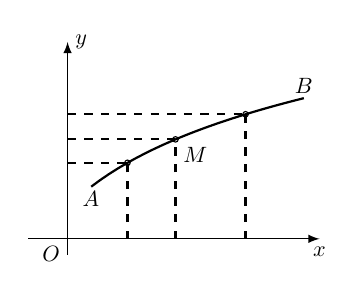
\begin{tikzpicture}
        \draw[-latex] (-0.5, 0) -- (3.2, 0) node[below,scale=0.8] {$x$};
        \draw[-latex] (0, -0.2) -- (0, 2.5) node[right,scale=0.8] {$y$};
        \node[below left,scale=0.8] (O) at (0, 0) {$O$};

        \node[below left,scale=0.8] (A) at (0.5, 0.7055) {$A$};
        \node[above,scale=0.8] (B) at (3, 1.75) {$B$};
        \node[below right,scale=0.8] (M) at (1.37, 1.2629) {$M$};

        \draw[domain=0.3:3, thick] plot (\x, {ln(\x+1)+0.4});

        \draw[dashed,thick] (0.76, 0) -- (0.76, 0.9653);
        \draw[dashed,thick] (1.37, 0) -- (1.37, 1.2629);
        \draw[dashed,thick] (2.26, 0) -- (2.26, 1.5817);
        \draw[dashed,thick] (0, 0.9653) -- (0.76, 0.9653);
        \draw[dashed,thick] (0, 1.2629) -- (1.37, 1.2629);
        \draw[dashed,thick] (0, 1.5817) -- (2.26, 1.5817);

        \draw (0.76, 0.9653) circle (1pt);
        \draw (1.37, 1.2629) circle (1pt);
        \draw (2.26, 1.5817) circle (1pt);
    \end{tikzpicture}
 \end{wrapfigure}
设函数 $y=f(x)$ 定义在某个区间 $\X$ 内.
在平面上取两条互相垂直的坐标轴, 对每一对满足 $x\in\X$、$y=f(x)$ 的数值,
作横坐标为 $x$、纵坐标为 $y$ 的点 $M(x,y)$.
当 $x$ 在 $\X$ 内变动时, 所有这些点组成的集合就是函数 $y=f(x)$ 的\emph{图像}.
在图示的情形中, 这些点画出一条曲线 $AB$;
这条曲线是函数的几何表示, 而方程 $y=f(x)$ 就称为曲线 $AB$ 的方程.

例如, 函数
$$
\begin{aligned}
y=\pm\sqrt{1-x^2}\quad (\abs{x}\leqslant1),\qquad
y=\pm\sqrt{x^2-1}\quad (\abs{x}\geqslant1)
\end{aligned}
$$
的图像分别是下方圆和等轴双曲线:

\begin{figure}[htbp]
    \vspace{-0.7cm}
    \centering
    \begin{minipage}[t]{0.44\textwidth}
        \centering
        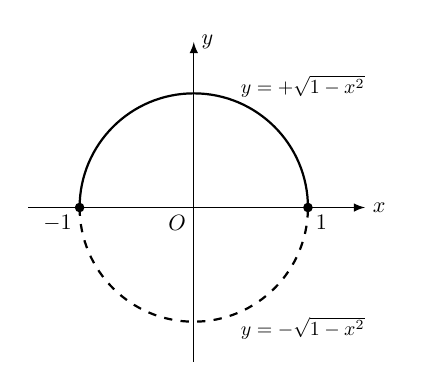
\begin{tikzpicture}[scale=1.45]
            \draw[-latex] (-1.45,0) -- (1.5,0) node[right,scale=0.8] {$x$};
            \draw[-latex] (0,-1.35) -- (0,1.45) node[right,scale=0.8] {$y$};
            \node[below left,scale=0.8] at (0,0) {$O$};
            \draw[thick] (1,0) arc[start angle=0,end angle=180,radius=1];
            \draw[dashed,thick] (-1,0) arc[start angle=180,end angle=360,radius=1];
            \fill (-1,0) circle (1.2pt);
            \fill (1,0) circle (1.2pt);
            \node[above right,scale=0.72] at (0.35,0.9) {$y=+\sqrt{1-x^2}$};
            \node[below right,scale=0.72] at (0.35,-0.9) {$y=-\sqrt{1-x^2}$};
            \node[below left,scale=0.8] at (-1,0) {$-1$};
            \node[below right,scale=0.8] at (1,0) {$1$};
        \end{tikzpicture}
    \end{minipage}
    \hfill
    \begin{minipage}[t]{0.48\textwidth}
        \centering
        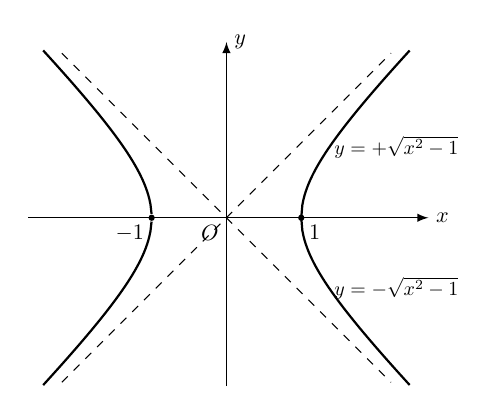
\begin{tikzpicture}[scale=0.95]
            \draw[-latex] (-2.65,0) -- (2.7,0) node[right,scale=0.8] {$x$};
            \draw[-latex] (0,-2.25) -- (0,2.35) node[right,scale=0.8] {$y$};
            \node[below left,scale=0.8] at (0,0) {$O$};
            \draw[dashed] (-2.2,-2.2) -- (2.2,2.2);
            \draw[dashed] (-2.2,2.2) -- (2.2,-2.2);
            \draw[domain=1:2.45,samples=100,thick] plot (\x,{sqrt(\x*\x-1)});
            \draw[domain=1:2.45,samples=100,thick] plot (\x,{-sqrt(\x*\x-1)});
            \draw[domain=-2.45:-1,samples=100,thick] plot (\x,{sqrt(\x*\x-1)});
            \draw[domain=-2.45:-1,samples=100,thick] plot (\x,{-sqrt(\x*\x-1)});
            \fill (-1,0) circle (1.2pt);
            \fill (1,0) circle (1.2pt);
            \node[above right,scale=0.72] at (1.35,0.7) {$y=+\sqrt{x^2-1}$};
            \node[below right,scale=0.72] at (1.35,-0.7) {$y=-\sqrt{x^2-1}$};
            \node[below left,scale=0.8] at (-1,0) {$-1$};
            \node[below right,scale=0.8] at (1,0) {$1$};
        \end{tikzpicture}
    \end{minipage}
\end{figure}

\begin{wrapfigure}[10]{r}{0.45\textwidth}
    \vspace{-0.5cm}
    \centering
    \begin{tikzpicture}[scale=0.85]
        \draw[-latex] (-2.65,0) -- (3.55,0) node[right,scale=0.8] {$x$};
        \draw[-latex] (0,-2.65) -- (0,2.85) node[right,scale=0.8] {$y$};
        \node[below left,scale=0.8] at (0,0) {$O$};
        \foreach \x in {-2,-1,1,2,3}{
            \draw (\x,0.08) -- (\x,-0.08) node[below] {$\x$};
        }
        \foreach \k in {-2,-1,0,1,2}{
            \draw[thick] (\k,\k) -- (\k+1,\k);
            \fill (\k,\k) circle (1.8pt);
            \draw[fill=white] (\k+1,\k) circle (1.8pt);
        }
        \node[left,scale=0.8] at (0,-2) {$-2$};
        \node[left,scale=0.8] at (0,-1) {$-1$};
        \node[left,scale=0.8] at (0,1) {$1$};
        \node[left,scale=0.8] at (0,2) {$2$};
        \node[above left,scale=0.8] at (-0.25,2.15) {$y=\floor{x}$};
    \end{tikzpicture}
\end{wrapfigure}
函数图像通常是逐点画出的.
在区间 $\X$ 内取一系列彼此接近的自变量值,
依公式 $y=f(x)$ 算出相应的函数值:
$$
\begin{array}{c|ccccc}
x= & x_1 & x_2 & x_3 & \cdots & x_n\\ \hline
y= & y_1 & y_2 & y_3 & \cdots & y_n
\end{array}
$$
再把点
$$
(x_1,y_1),\ (x_2,y_2),\ \ldots,\ (x_n,y_n)
$$
画在图上, 用光滑的线段连接作出曲线.
这样得到的曲线虽然只是所求图像的近似,
但是曲线画得越光滑, 所取的点越稠密, 它就越准确地表示函数的图像.

必须注意, 虽然常用几何图形来表示函数,
函数的图像却不一定是通常直观意义下的曲线.
例如, 取整函数 $y=\floor{x}$ 在每个区间 $[m,m+1)$ ($m$ 取一切整数) 内都保持常值 $m$,
因而它的图像由一系列左端点属于图像、右端点不属于图像的水平线段组成.
至于 Dirichlet 函数 $D(x)$,
它的图像由直线 $y=1$ 上横坐标为有理数的点,
以及 $x$ 轴上横坐标为无理数的点组成, 这种图像却无法实际画出.

\subsection{几类重要的函数}

	%\include{text/chapter3}

% =================新增的打印索引=================
    \backmatter
    \printindex         % 打印名词索引
    %\printindex[names]  % 打印人名索引
% ==============================================
\end{document}
